% !Mode:: "TeX:UTF-8"
%!TEX program  = xelatex
% ============================================================
% 华为杯（中国研究生数学建模竞赛）论文主稿
% 版式由 gmcmthesis.cls 提供，本文件只负责内容组织与门禁标签。
% 全部数值以宏形式给出，宏定义在 论文/数值.tex 中由脚本自动生成。
% ============================================================
\documentclass[bwprint]{gmcmthesis}

\hypersetup{hidelinks, allcolors=black}

\usepackage{subfig}
\usepackage{siunitx}

\counterwithout{figure}{section}
\counterwithout{table}{section}

\usepackage[noend]{algpseudocode}
\usepackage{algorithmicx,algorithm}
\floatname{algorithm}{算法}
\renewcommand{\algorithmicrequire}{\textbf{输入:}}
\renewcommand{\algorithmicensure}{\textbf{输出:}}

\makeatletter
\def\@cite#1#2{\textsuperscript{[{#1\if@tempswa , #2\fi}]}}
\makeatother

% 本文件由 scripts/fill_paper_numbers.py 从 results/final_results.json 自动生成。
% 论文正文只引用这些宏，禁止在正文中硬编码数值。

\newcommand{\CaseCount}{100}
\newcommand{\CoreRange}{1 至 5}
\newcommand{\CoreFive}{五}
\newcommand{\OpsMin}{552}
\newcommand{\OpsMax}{35705}
\newcommand{\OpsMed}{3720}
\newcommand{\CyclesMin}{23052}
\newcommand{\CyclesMax}{61275840}
\newcommand{\LevelMed}{47}
\newcommand{\MatShareMed}{67.7\%}
\newcommand{\WidthMed}{43.1}
\newcommand{\QOneSpeedTwo}{1.246}
\newcommand{\QOneSpeedFive}{1.920}
\newcommand{\QTwoSpeedFive}{2.140}
\newcommand{\QThreeGainFive}{1.033}
\newcommand{\QThreeHitFive}{9.7\%}
\newcommand{\QThreeHitTwo}{5.2\%}
\newcommand{\TrafficDrop}{7.6\%}
\newcommand{\EstRatioMed}{0.66}
\newcommand{\TimelineGap}{6.8\%}
\newcommand{\BestBlocks}{1}
\newcommand{\MarginLow}{0.75}
\newcommand{\MarginHigh}{1.00}
\newcommand{\MarginSwing}{2.4\%}
\newcommand{\BestCombo}{1.74}


\newcommand{\CodeGraphUtils}{\texttt{graph\_utils.py}}
\newcommand{\CodePartition}{\texttt{partition.py}}
\newcommand{\CodeEvalRunner}{\texttt{eval\_runner.py}}
\newcommand{\CodeRunExperiments}{\texttt{run\_experiments.py}}
\newcommand{\CodeAggregate}{\texttt{aggregate\_results.py}}
\newcommand{\CodeBuildDataset}{\texttt{build\_dataset.py}}
\newcommand{\CodeFiguresQOne}{\texttt{figures\_q1.py}}
\newcommand{\CodeFiguresQTwo}{\texttt{figures\_q2.py}}
\newcommand{\CodeFiguresQThree}{\texttt{figures\_q3.py}}
\newcommand{\CodeSensitivityRun}{\texttt{run\_sensitivity.py}}
\newcommand{\CodeSensitivityFig}{\texttt{fig\_sensitivity.py}}
\newcommand{\CodeFinalResults}{\texttt{final\_results.json}}
\newcommand{\CodeCaseProfile}{\texttt{case\_profile.csv}}

\graphicspath{{../}{./}{figures/}{../figures/}}

%===================== 建模论文题目与封面信息 =====================

\title{通用神经网络处理器下的多核切图与调度建模}
\baominghao{\hspace{6em} 20260900001}
\schoolname{\hspace{5.8em} 学校名称填写}
\membera{\hspace{6em} 成员A}
\memberb{\hspace{6em} 成员B}
\memberc{\hspace{6em} 成员C}

%=======================================================

\begin{document}
\label{body:start}

\maketitle

\begin{abstract}\label{abstract:start}
多核神经网络处理器已成为突破单核算力与功耗瓶颈的主流架构，而把一张完整计算图
切分成子图、分配到各核心并确定核内执行顺序，直接决定任务时延与数据搬运开销。
本文把切图、分核与核内排序统一为一个以任务级完工时间为目标的组合优化问题，构造了
可证明无环的切分方案与以关键路径优先级驱动的分核算法，并在赛题官方评估程序上完成
了全部 \CaseCount 个测试用例、\CoreRange 核配置的完整实验。

\textbf{针对问题一}，本文把 Op-Tensor 二部图收缩为操作级有向无环图，用最长路径把操作分成
\LevelMed 层，发现矩阵流水线工作量占全部计算量的 \MatShareMed，而并行宽度
中位数达 \WidthMed 倍。基于“跨子图依赖图必须无环”这一硬约束，本文提出依赖锥
聚簇、连续段切分与分层切分三类构造：依赖锥聚簇让每个操作跟随承载最重上游分支的
主前驱，连续段切分先构造保持后代连续的拓扑序再按“跨切边数与负载偏差联合代价”
挑选切点，分层切分则按最长路径分层并把层内独立操作均衡撒到各核，三者的子图依赖
图都从构造上保证无环。分核阶段采用后向关键路径优先级排序，把子图分配到使估算
完工时间最小的核心，并用单核兜底锁定下界。场景 A 下 \CoreFive 核平均加速比达到
\textbf{\QOneSpeedFive 倍}。

\textbf{针对问题二}，本文重新刻画场景 B 的代价结构：同一核心的全部子图合并为一个任务，
同核数据在私有缓存中直接复用，只有跨核边才插入搬运并支付 500 周期同步延迟。
入向边界搬运因此只统计跨核部分，分核阶段按新代价重新均衡负载。\CoreFive 核平均
加速比提高到 \textbf{\QTwoSpeedFive 倍}，额外搬运量相对场景 A 下降 \TrafficDrop，
说明核内驻留确实减少了共享主存流量。

\textbf{针对问题三}，本文建立只读 L2 的复用模型：一份被 $g$ 个核心读取的张量，首次访问
未命中、其后 $g-1$ 次命中，有效读入代价为 $\frac{s}{\mathrm{BW}_{\mathrm{ddr}}}
+(g-1)\frac{s}{\mathrm{BW}_{\mathrm{L2}}}$。据此把切分阶段的入向有效带宽由 60
改为 250 字节/周期，得到 L2 感知切分；同时保留 DDR 口径切分作为对照，逐用例实测
择优。\CoreFive 核下只读 Cache 相对无 L2 基线的平均加速比为 \textbf{\QThreeGainFive 倍}，
平均 Cache 命中率为 \QThreeHitFive。

本文的主要贡献是把“子图依赖图无环”从校验条件提升为构造约束，使切分与分核可以在
同一目标函数下联合优化；同时用单核兜底把算法的下界锁定在不劣化于单核基线的水平。
灵敏度分析表明，每个核心的子图数取 \BestBlocks 时平均加速比最高，单核兜底阈值
在 \MarginLow 至 \MarginHigh 区间内结果稳定。

\keywords{多核调度\quad 计算图切分\quad 有向无环图\quad 列表调度\quad 只读缓存复用}\label{abstract:end}

\end{abstract}

\pagestyle{plain}

\maketoc
\clearpage

% ============================================================
\section{问题重述}

\subsection{问题背景}

人工智能模型规模持续增长，单个 AI 核心受制造成本、功耗与散热约束，难以独立满足
算力需求，多核 NPU 因此成为提升并行能力与能效的主流架构。多核 NPU 平台由若干同构
AI 核心与共享核外主存构成：每个核心配有 Cube 矩阵计算单元、Vector 向量计算单元、
两类数据搬运单元以及私有的 L1 与 UB 缓存；所有核心对主存的读写共同竞争固定的总
物理带宽。硬件结构与整体技术路线见图~\ref{fig:roadmap}。

把一张完整计算图真正跑起来，需要回答三个相互耦合的问题：哪些操作应当被划入同一个
子图，每个子图应当交给哪个核心，以及同一核心上的子图按什么顺序执行。切图改变子图
规模、并行空间与通信边界；核心分配决定负载均衡与跨核通信量；核内顺序影响依赖等待、
张量驻留时间与缓存换入换出。三者不能孤立优化：切分越细，并行机会越多，但跨子图
搬运与重复读取也随之增加；聚合越多，通信越省，但并行度被压缩、缓存压力上升。

本文要处理的计算图是一张 Op-Tensor 二部图：张量节点表示输入、中间结果与输出，
操作节点表示计算或搬运，有向边只允许张量与操作相连。输入输出张量位于核外主存，
中间张量的逻辑位置为核内缓存。评测以总体任务执行时间（Makespan）为首要指标，
以总额外数据搬运量为次要指标，问题三还额外统计只读 Cache 命中率。

\subsection{问题提出}

赛题给出 \CaseCount 个测试用例与一份固定配置，要求分别在三类硬件场景下建立多核
切图与调度模型、设计求解算法，并在全部用例、1 至 5 核范围内给出稳定高效的结果。

场景 A 没有核间同步机制，一个任务只能包含一个子图，子图间的同步由主控通过任务
调度完成；同一核心上多个任务串行执行时核内缓存被清空，因此所有跨子图数据都必须
经主存中转，即使两个子图位于同一核心也是如此。

场景 B 存在核间同步机制，一个任务可以包含同一核心上的多个子图，前序子图的数据
可以驻留在 L1 或 UB 中供后续子图直接使用；跨核依赖由源核心写入主存并发送同步信号，
目标核心收到信号后再读取，因此同核单位通信成本低于跨核成本。

问题三在场景 B 的基础上引入所有核心共享的只读二级缓存，容量 1 MB，带宽
250 字节/周期，用于复用多核共享输入，其带宽与主存带宽相互独立。

三个问题的输出都是同一套方案格式：一张把每个核内操作映射到子图编号的映射表，
以及一组按核心给出的子图执行顺序列表。赛题提供的评估程序会据此重建跨子图边界的
数据搬运、确定核内操作顺序、模拟多核在共享带宽下的并行执行，并给出各项指标。
方案合法性的硬条件包括：映射表必须恰好覆盖全部非搬运操作，每个子图必须且只能被
调度一次，子图依赖图必须无环，同一核心上的子图顺序不得违反依赖关系。

\subsection{整体求解路线}

本文的整体技术路线见图~\ref{fig:roadmap}。输入与建模基础部分完成计算图解析、
操作级有向无环图收缩与结构画像；三问目标与对应模型算法部分给出各自的代价口径与
求解算法；实验验证与结果交付部分用官方评估程序复核全部用例，再做灵敏度分析与
结果聚合。问题分析结构见图~\ref{fig:analysis}，图中给出了题目给定的耦合结构、
必须同时满足的硬约束、解耦思路与算法主线的真实回环。

\begin{figure}[H]
\centering
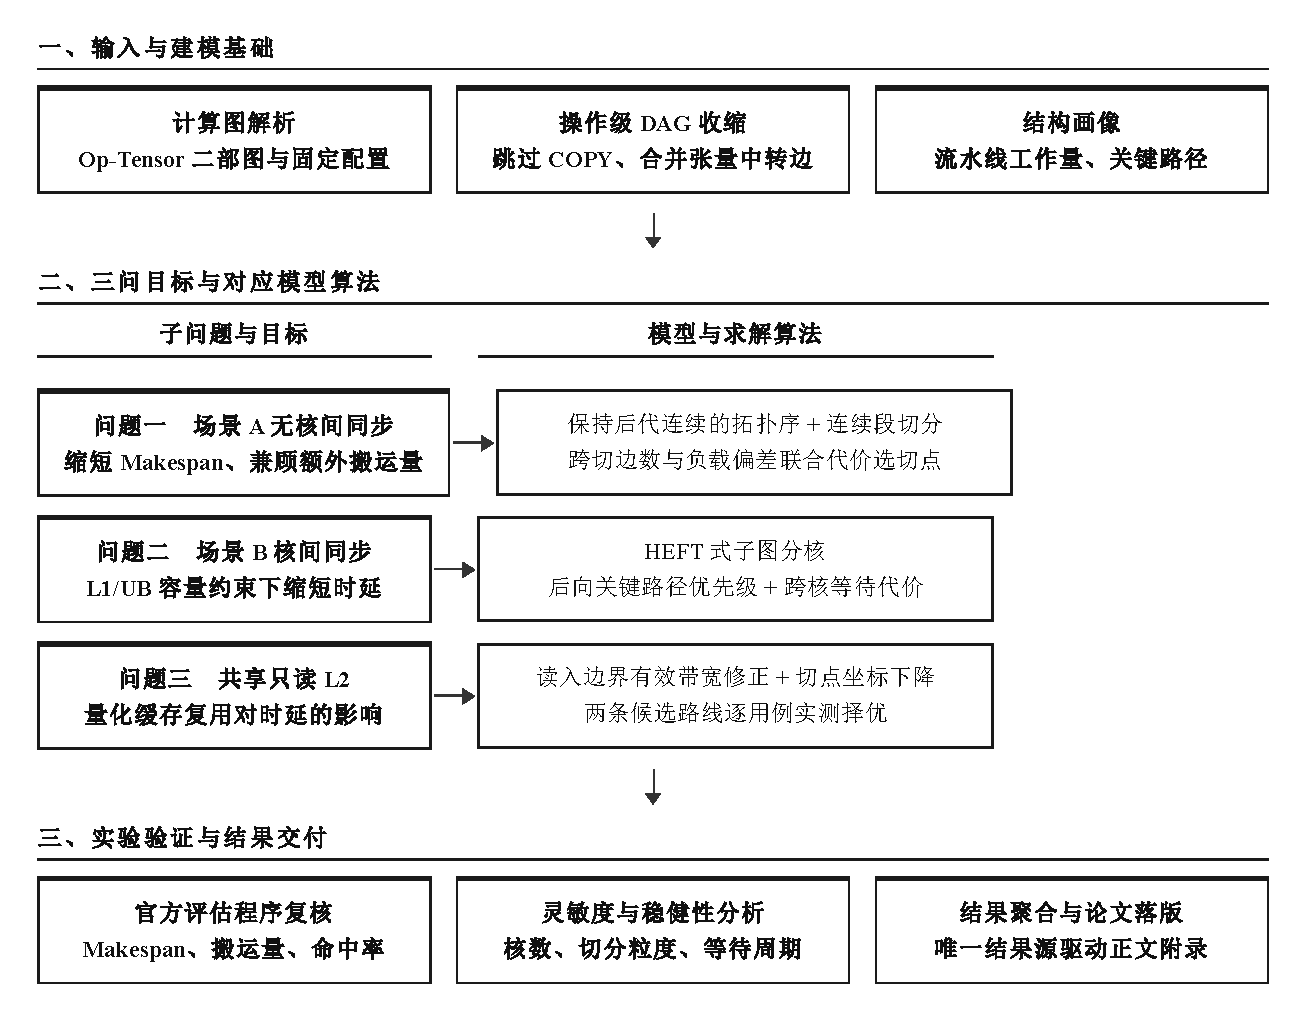
\includegraphics[width=\textwidth,height=0.7\textheight,keepaspectratio]{手绘图/fig_roadmap.pdf}
\caption{整体技术路线图}\label{fig:roadmap}
\end{figure}

技术路线把三问的共同基础与差异分开：三问共享同一套“操作级有向无环图收缩 + 无环
切分构造 + 关键路径优先级分核”的骨架，差异只体现在代价口径与等待常数上。这样
问题二与问题三可以在问题一的算法上增量修改，而不必重新设计求解框架。

\begin{figure}[H]
\centering
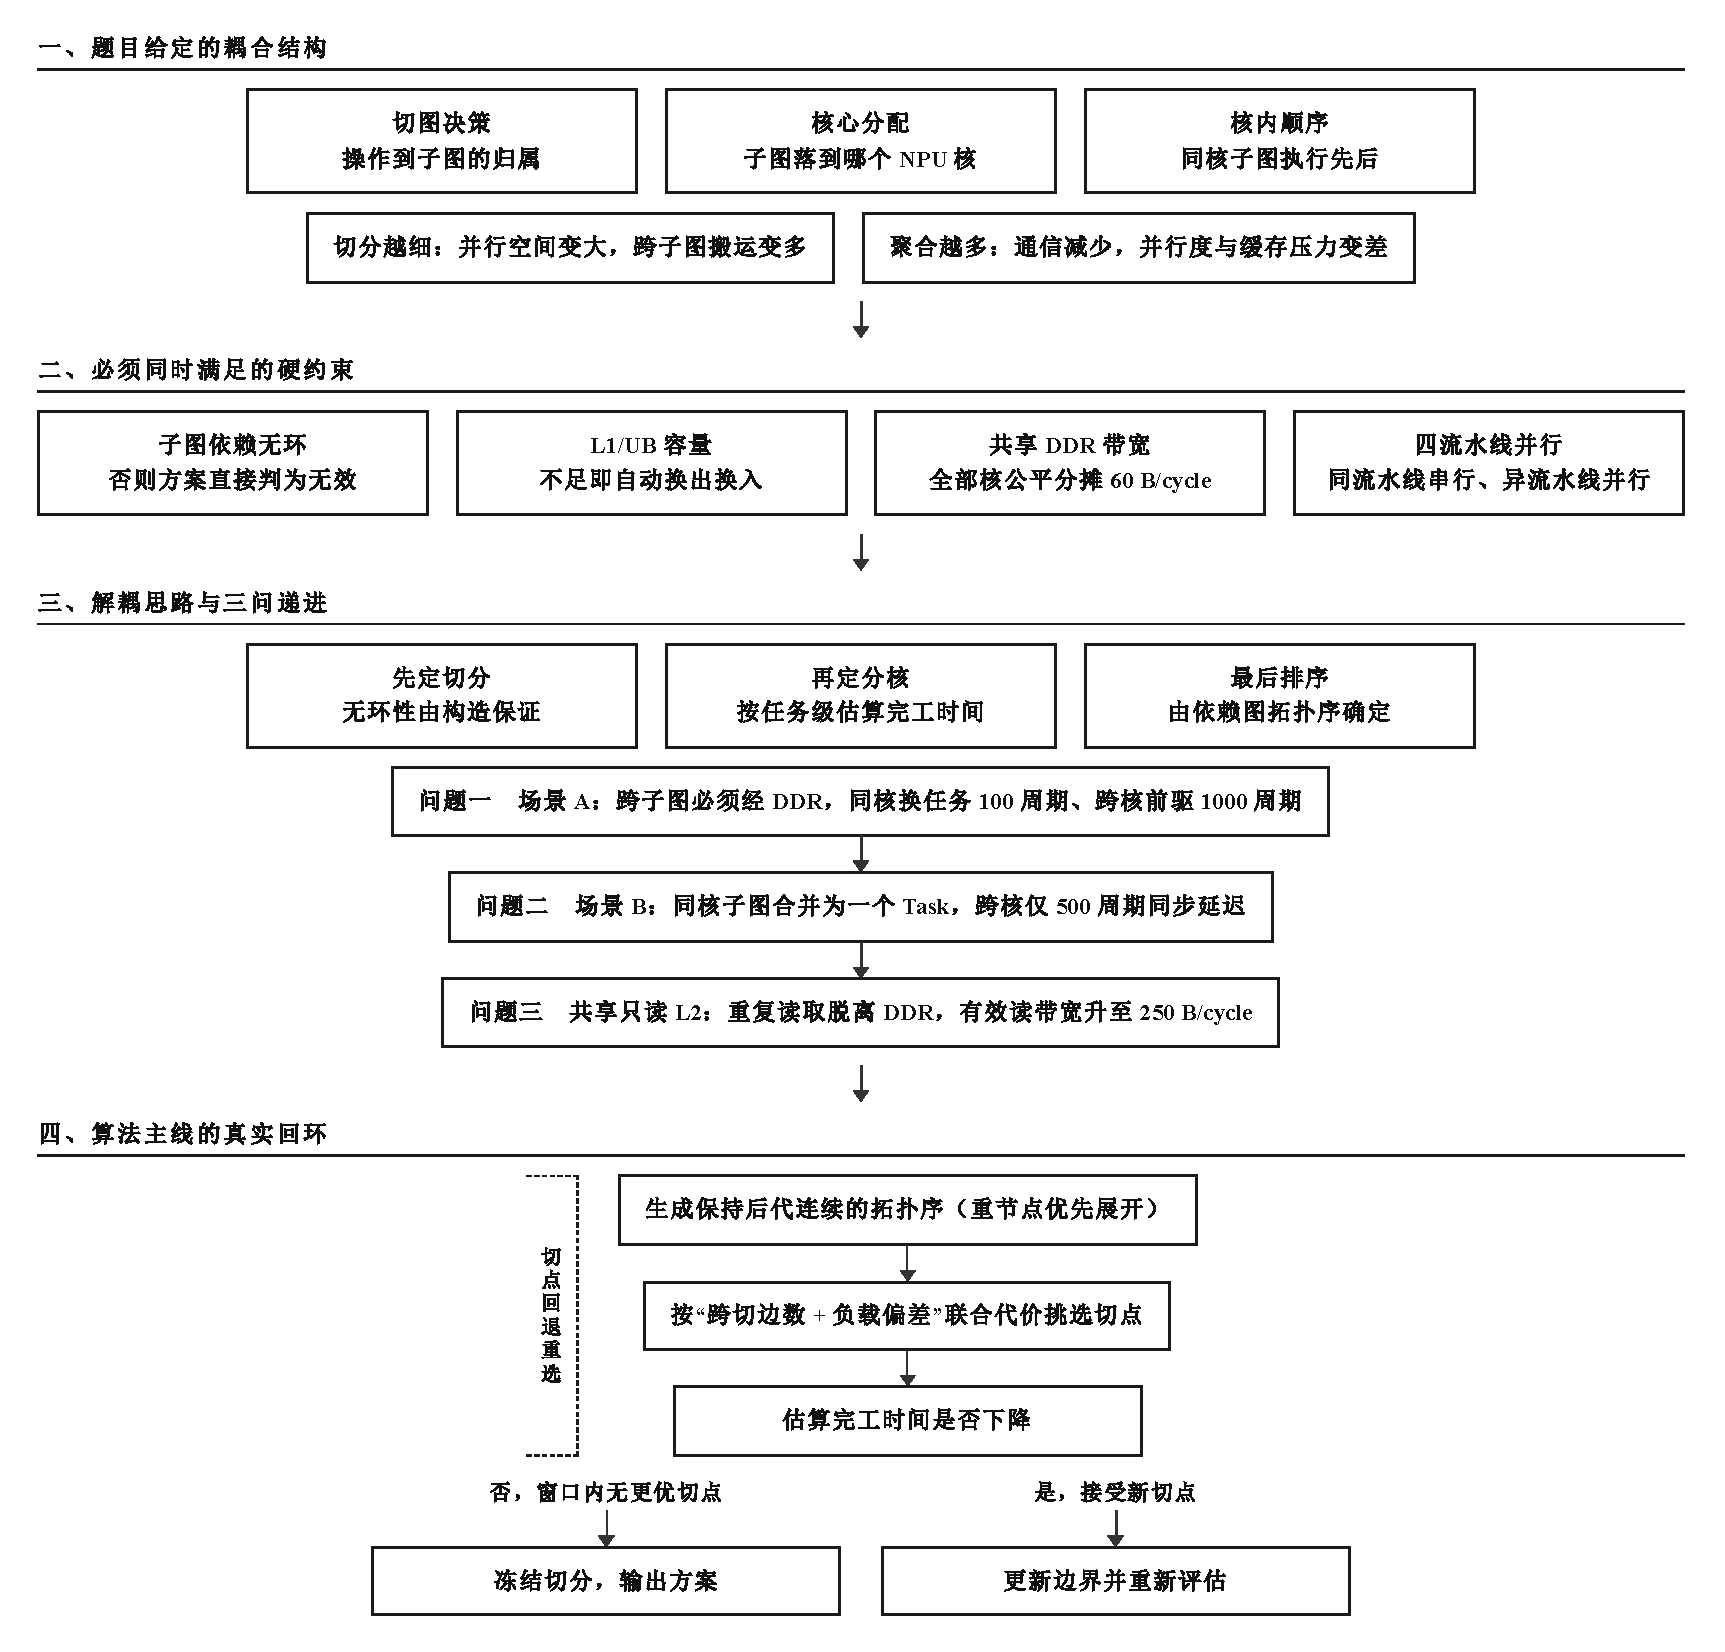
\includegraphics[width=0.86\textwidth,height=0.6\textheight,keepaspectratio]{手绘图/fig_analysis.pdf}
\caption{问题分析流程图}\label{fig:analysis}
\end{figure}

\section{模型假设与符号说明}

\subsection{模型假设}

\begin{enumerate}
\item 平台由 $N$ 个同构核心构成，各核心的计算能力与私有缓存容量完全相同，因此
负载均衡只取决于分配到各核的工作量，而与核心身份无关。
\item 计算图在调度前已完全确定且无环，图的规模与拓扑在运行期不发生变化。
\item 全部调度决策在执行前一次性确定，运行期不做重调度，因此本文方法属于静态调度。
\item 子图内部四条流水线相互独立：同一条流水线上的操作串行执行，不同流水线可以
并行推进；子图时长下界取各流水线工作量与核内关键路径的最大值。
\item 跨子图边界的搬运字节数由承载该依赖的张量大小决定，与边的条数无关；边本身
不重复存储通信量。
\item 访问核外主存的搬运共享同一条物理带宽，多个核心的并发搬运按并发数公平分摊，
本文以字节数与带宽之比折算时间。
\item 场景 A 中同核换任务等待为 100 周期、跨核前驱等待为 1000 周期；场景 B 中
跨核拷贝同步延迟为 500 周期。这些常数由赛题固定配置给出，不作为决策变量。
\item 核内缓存容量不足时，由官方核内调度算法自动插入缓存换出与换入，本文不改变
该机制，只在代价估算中考虑其带来的额外搬运。
\item 问题三的只读 Cache 按先进先出淘汰，命中访问不改变队列顺序；单个张量大于
Cache 容量时不缓存。该行为由官方评估程序实现，本文只在建模层面刻画其影响。
\item 官方评估程序给出的 Makespan 是唯一权威指标，本文的一切结论都以该程序的
输出为准，估算模型只用于算法内部的搜索与择优。
\end{enumerate}

\subsection{符号说明}

以下符号贯穿全文，含义与单位保持一致；同一符号在不同问题中若含义不同，会在对应
章节重新声明。

\renewcommand\arraystretch{1.2}
\newcolumntype{L}{>{\quad}X}
\newcolumntype{P}[1]{>{\centering\arraybackslash}p{#1}}
\newcounter{huaweisymbolsavetable}
\setcounter{huaweisymbolsavetable}{\value{table}}
\begin{longtable}{|P{2.4cm}|>{\raggedright\arraybackslash}p{\dimexpr0.92\textwidth-2.4cm-4\tabcolsep-3\arrayrulewidth\relax}|}
  \hline
  符号    &   \quad 意义 \\
  \hline
  \endfirsthead
  \hline
  符号    &   \quad 意义（续） \\
  \hline
  \endhead
  \hline
  \endfoot
  $G=(V,E)$  &  计算图，$V=T\cup O$ 为张量节点与操作节点之并 \\
  \hline
  $T,\;O$  &  张量节点集合与操作节点集合，二者不相交 \\
  \hline
  $s_t$  &  张量 $t$ 占用的字节数 \\
  \hline
  $c_o$  &  核内计算操作 $o$ 的执行周期数 \\
  \hline
  $N$  &  参与调度的同构核心数，取值范围为 1 至 5 \\
  \hline
  $w_v$  &  操作 $v$ 折算后的工作量权重，取该操作的周期数 \\
  \hline
  $w^{M}_v,\;w^{V}_v$  &  操作 $v$ 在矩阵流水线与向量流水线上的周期数 \\
  \hline
  $\sigma$  &  用于切分的拓扑序，$\sigma(i)$ 表示序列中第 $i$ 个操作 \\
  \hline
  $b_0<b_1<\cdots<b_N$  &  切点边界，第 $k$ 段为 $\sigma[b_{k-1}:b_k]$ \\
  \hline
  $G_k$  &  第 $k$ 个子图所包含的操作集合 \\
  \hline
  $X(p)$  &  在序列位置 $p$ 处切开时的跨切边数 \\
  \hline
  $M_k,\;V_k$  &  子图 $k$ 的矩阵流水线与向量流水线工作量 \\
  \hline
  $B^{\mathrm{in}}_k,\;B^{\mathrm{out}}_k$  &  子图 $k$ 的入向与出向边界搬运字节数 \\
  \hline
  $D_k$  &  子图 $k$ 的估算时长 \\
  \hline
  $c_k$  &  子图 $k$ 被分配到的核心编号 \\
  \hline
  $\mathrm{rank}(k)$  &  子图 $k$ 的后向关键路径长度 \\
  \hline
  $\Delta(c_i,c_k)$  &  两个子图分处不同核或同核时的固定等待周期 \\
  \hline
  $\mathrm{BW}_{\mathrm{ddr}}$  &  共享主存总带宽，取 60 字节/周期 \\
  \hline
  $\mathrm{BW}_{\mathrm{L2}}$  &  只读 Cache 命中带宽，取 250 字节/周期 \\
  \hline
  $g(t)$  &  张量 $t$ 的消费者所分布的核心数 \\
  \hline
  $h$  &  只读 Cache 命中率，命中字节与总访问字节之比 \\
  \hline
  $\mathrm{Cap}$  &  核内缓存容量，L1 取 524288 字节、UB 取 131072 字节 \\
  \hline
\end{longtable}
\setcounter{table}{\value{huaweisymbolsavetable}}

% ============================================================
\section{问题一模型建立与求解}

\subsection{问题分析与建模思路}

场景 A 的评估语义可以概括为一句话：每个子图独立构成一个任务，任务之间不保留
核内数据，任何跨子图数据都必须经主存中转。由此可以写出任务 $k$ 的最早激活时刻

\begin{equation}
t_k=\max\Bigl(\underbrace{\mathrm{free}(c_k)}_{\text{同核换任务}},
\;\underbrace{\max_{i\to k}\bigl(t_i+D_i+\Delta(c_i,c_k)\bigr)}_{\text{依赖等待}}\Bigr),
\qquad
\Delta(c_i,c_k)=
\begin{cases}
100, & c_i=c_k,\\
1000, & c_i\neq c_k,
\end{cases}
\end{equation}

其中同核换任务等待 100 周期、跨核前驱等待 1000 周期均由固定配置给出。式 (1) 说明
场景 A 的优化目标不是单纯缩短各核工作量，而是要让依赖链尽量落在同一核心上，
避免在关键路径上反复支付跨核等待。

这里出现了一个容易被忽略的硬约束。若把操作任意分配到各核心，商图（把每个子图
缩成一个点的依赖图）可能出现环，例如子图 $A$ 中的操作依赖子图 $B$ 中的操作，
同时子图 $B$ 中又有操作依赖子图 $A$ 中的操作。此时两个任务互相等待，方案直接
被判为无效。因此本文把“子图依赖图无环”从方案校验条件提升为切分构造约束，
先保证无环，再在该约束下优化完工时间。

另一个需要事先判明的因素是问题本身的可并行程度。对每个用例定义并行宽度

\begin{equation}
\mathrm{PW}=\frac{\sum_{v\in V}w_v}{\max_{v\in V}\mathrm{CP}(v)},
\end{equation}

其中 $\mathrm{CP}(v)$ 是以操作 $v$ 结尾的最长加权路径。$\mathrm{PW}$ 是加速比的
上界：当 $\mathrm{PW}$ 接近 1 时用例本质串行，任何切分都无法带来收益，算法必须
在此时保持不劣化，否则会给出比单核更差的方案。

\subsection{计算图预处理与结构画像}

把 Op-Tensor 二部图收缩为操作级有向无环图的做法是：张量中转边合并为操作之间的
直接依赖，搬运操作作为中转节点被跳过。设操作 $u$ 经若干张量节点可达操作 $v$，
则在操作级图中加入边 $u\to v$。收缩后得到仅含核内操作的依赖关系，记其前驱集合
为 $\mathrm{pred}(v)$。

对全部 \CaseCount 个用例统计得到：核内操作数从 \OpsMin 到 \OpsMax，
中位数 \OpsMed；总工作量从 \CyclesMin 到 \CyclesMax 周期；最长路径层数
中位数 \LevelMed；矩阵流水线工作量占比中位数 \MatShareMed；并行宽度中位数
\WidthMed 倍。图~\ref{fig:dataset_profile} 给出四幅结构画像：并行宽度随规模的
分布、主存张量总量分布、矩阵流水线工作量占比分布，以及关键路径与总工作量的
对应关系。

\begin{figure}[H]
\centering
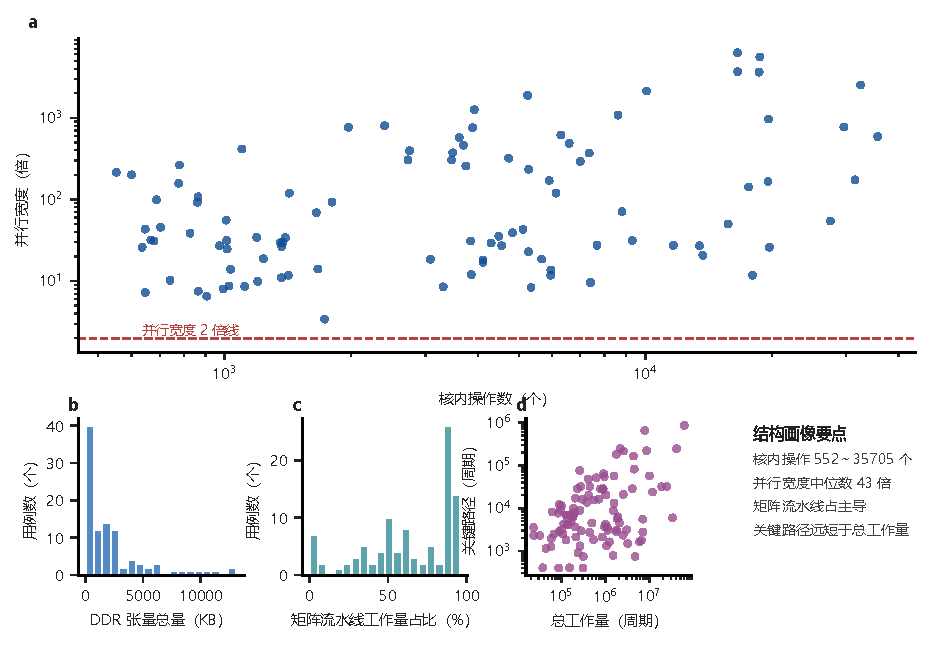
\includegraphics[width=\textwidth,height=0.66\textheight,keepaspectratio]{数据预处理/figures/fig_dataset_profile.pdf}
\caption{测试用例结构画像}\label{fig:dataset_profile}
\end{figure}

图~\ref{fig:dataset_profile} 的 (a) 面板显示并行宽度与规模基本无关，说明图越大
并不自动越容易并行；(d) 面板显示关键路径比总工作量低一到两个数量级，说明多数
用例的瓶颈不是依赖链本身，而是工作量在核心之间的分配与跨核等待的累积。

把每个用例按最长路径分层后，可以进一步观察工作量在层间的分布。
图~\ref{fig:dag_layers} 对总工作量最大的 12 个用例给出归一化分层后的工作量占比
热图。

\begin{figure}[H]
\centering
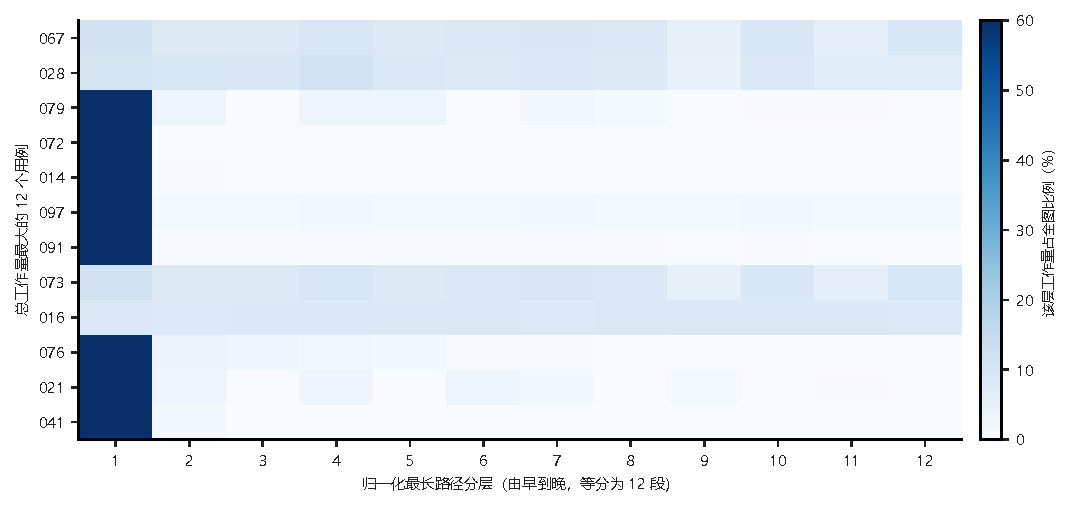
\includegraphics[width=\textwidth,height=0.5\textheight,keepaspectratio]{数据预处理/figures/fig_dag_layers.pdf}
\caption{分层工作量占比分布}\label{fig:dag_layers}
\end{figure}

图~\ref{fig:dag_layers} 显示工作量高度集中在最早的分层：若干用例的第一层就占用了
全部工作量的四成以上。这一结构决定了切分策略的取向，因为最早的分层内部操作相互
独立，把它们均衡地撒到各核心即可获得大部分并行收益，而后续分层的汇合点必须与
其生产者放在同一核心，否则会在关键路径上引入跨核等待。

\subsection{无环切分模型}

切分决策由拓扑序 $\sigma$ 与切点边界 $b_0<b_1<\cdots<b_N$ 共同确定，第 $k$ 个
子图为 $\sigma$ 上的连续段 $\sigma[b_{k-1}:b_k]$。这样构造的商图必然无环，因为
任意跨段边都沿 $\sigma$ 正向，子图编号本身就是商图的一个拓扑序。这一性质把无环性
从需要事后校验的约束变成了构造性保证。

切点选择要在“少跨边”与“负载均衡”之间权衡。定义位置 $p$ 处的跨切边数

\begin{equation}
X(p)=\bigl|\{(u,v)\in E\ \text{且}\ \mathrm{pos}(u)<p\le \mathrm{pos}(v)\}\bigr|,
\end{equation}

以及第 $k$ 段偏离平均工作量的相对偏差

\begin{equation}
\mathrm{dev}(p)=\frac{\bigl|W(b_{k-1},p)-\bar W\bigr|}{\bar W},
\qquad
W(a,p)=\sum_{i=a}^{p-1}w_{\sigma(i)},
\qquad
\bar W=\frac{1}{N}\sum_{v\in V}w_v .
\end{equation}

切点在以 $X(p)$ 为主、以 $\mathrm{dev}(p)$ 为次的字典序下挑选，并限制段工作量落在
平均值的 0.7 至 1.35 倍区间内。限制区间的意义在于避免出现“为了压低跨边数而切出
极小段”的退化情形。

子图时长按四条流水线的并行结构估算。记子图 $k$ 的入向边界字节 $B^{\mathrm{in}}_k$、
出向边界字节 $B^{\mathrm{out}}_k$，则

\begin{equation}
D_k=\max\Bigl(M_k,\;V_k,\;\frac{B^{\mathrm{in}}_k}{\mathrm{BW}_{\mathrm{in}}},\;
\frac{B^{\mathrm{out}}_k}{\mathrm{BW}_{\mathrm{ddr}}},\;\mathrm{CP}_k\Bigr),
\end{equation}

其中 $\mathrm{CP}_k$ 为子图内部的关键路径。入向有效带宽 $\mathrm{BW}_{\mathrm{in}}$
在问题一取主存带宽，在问题三取只读 Cache 命中带宽，这一处替换正是问题三建模的
切入点。

除连续段切分之外，本文还构造了依赖锥聚簇作为候选方案。其做法是先按可达工作量
计算每个操作的主前驱

\begin{equation}
\mathrm{prim}(v)=\arg\max_{p\in \mathrm{pred}(v)}\;\mathrm{down}(p),
\qquad
\mathrm{down}(p)=w_p+\sum_{q\in \mathrm{succ}(p)}\mathrm{down}(q),
\end{equation}

再把全部源操作按工作量均衡地撒到各核心，其余操作跟随其主前驱所在核。依赖锥聚簇
在“一个重操作扇出到大量轻操作”的用例上表现很好，因为扇出结构被完整保留在同一
核内；但它不保证商图无环，需要用环修复过程处理。

第三类构造是分层切分。把所有操作按最长路径分层后，层内操作之间没有依赖边，
而所有依赖边都从低层指向高层。若把每个分层单独作为一组子图、按层递增编号，则
子图依赖图必然无环，核心分配也就不再受无环性约束，可以在保持合法性的同时自由
追求负载均衡。记层 $\ell$ 的操作集合为 $L_\ell$，其工作量 $W_\ell=\sum_{v\in L_\ell}w_v$，
分层切分把 $L_\ell$ 内部按工作量切成若干块并分配到当前累计负载最小的核心：

\begin{equation}
c\bigl(L_\ell^{(j)}\bigr)=\arg\min_{c\in\{0,\dots,N-1\}}
\sum_{\ell'<\ell}\;\sum_{j'}W_{\ell'}^{(j')}\,
\mathbf{1}\bigl[c\bigl(L_{\ell'}^{(j')}\bigr)=c\bigr].
\end{equation}

式 (8) 的贪心规则使各核的累计工作量尽量接近。分层切分的代价是层与层之间形成
一条链，层 $\ell+1$ 必须等层 $\ell$ 全部完成才能开始，因此它适合工作量集中在少数
宽层的用例，而不适合层数很多且每层都很薄的深图。

\subsection{子图分核模型}

分核阶段以式 (1) 的激活时刻模型为目标。对每个子图定义后向关键路径长度

\begin{equation}
\mathrm{rank}(k)=D_k+\max_{k\to j}\mathrm{rank}(j),
\end{equation}

按 $\mathrm{rank}$ 降序处理子图，把每个子图分配到使其估算完成时刻最小的核心：

\begin{equation}
c_k=\arg\min_{c\in\{0,\dots,N-1\}}
\Bigl[\max\Bigl(\mathrm{free}(c),\;\max_{i\to k}\bigl(t_i+D_i+\Delta(c_i,c)\bigr)\Bigr)+D_k\Bigr].
\end{equation}

式 (10) 是经典的异构最早完成时间准则在本题上的实例化：它同时考虑了核心的空闲
时刻与依赖链上的等待，因此不会把互相依赖的子图拆到不同核心上徒增跨核等待。
分配到核心 $c$ 后更新 $\mathrm{free}(c)$，并继续处理下一个子图。

需要强调的是，分核只在估算层面进行，最终指标始终由官方评估程序给出。估算模型
的作用是提供搜索方向，而不是替代评估。估算模型还必须显式计入全局主存带宽下界：
切分引入的边界搬运与原始搬运共享同一条主存带宽，因此估算完工时间取任务级流水
估算与总搬运字节数除以主存带宽两者中的较大者。这一项对细切分尤为关键，因为细
切分虽然缩短了各核的计算时间，却可能把主存带宽变成真正的瓶颈。

\subsection{求解算法}

完整求解流程见图~\ref{fig:flow_q1}。算法先做图预处理，再并行构造三类候选切分，
按估算完工时间择优，最后用单核兜底锁定下界。

\begin{figure}[H]
\centering
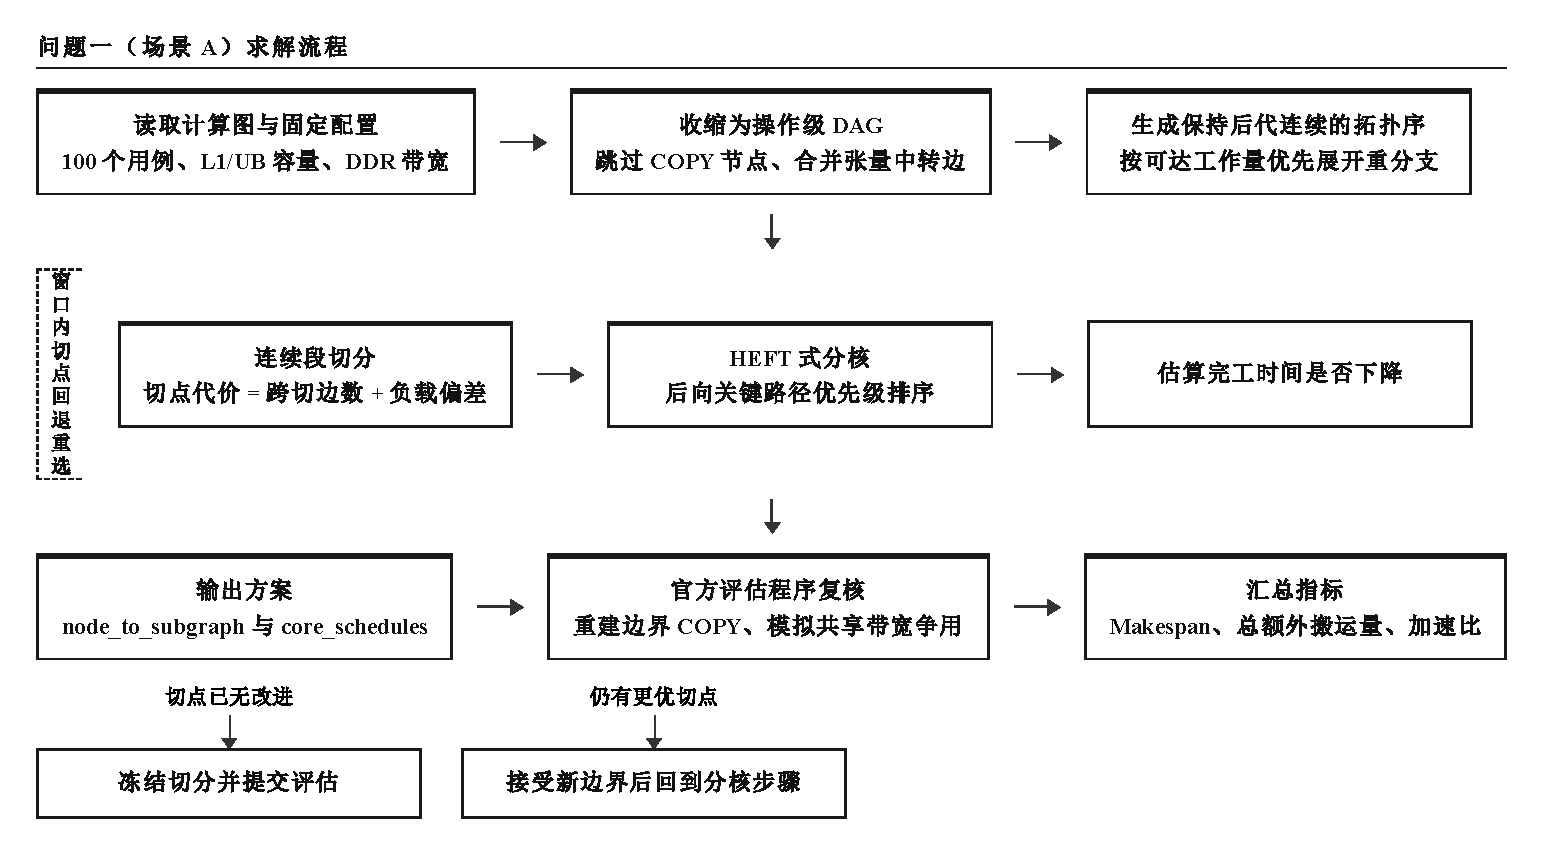
\includegraphics[width=\textwidth,height=0.58\textheight,keepaspectratio]{手绘图/fig_flow_q1.pdf}
\caption{问题一求解流程图}\label{fig:flow_q1}
\end{figure}

算法 1 给出完整的求解步骤。其中第 2 至 4 行分别对应三类候选构造，它们分别适合
扇出结构、链式结构与宽层结构；第 8 行的单核兜底则保证算法不会给出比单核基线更差
的方案。

\begin{algorithm}[H]
\caption{场景 A 多核切图与调度算法}
\begin{algorithmic}[1]
\Require 计算图 $G=(V,E)$，核心数 $N$，跨核等待 $\Delta_{\times}$，同核等待 $\Delta_{\parallel}$
\Ensure 方案：操作到子图的映射表，各核的子图执行顺序
\State 把 $G$ 收缩为操作级有向无环图，计算 $w^{M}_v$、$w^{V}_v$ 与 $\mathrm{down}(v)$
\State 候选一：按式 (7) 计算主前驱，源操作均衡撒开，其余操作跟随主前驱，得到依赖锥聚簇
\State 候选二：构造保持后代连续的拓扑序，按式 (3)(4) 的联合代价挑选切点，得到连续段切分
\State 候选三：按最长路径分层，层内操作独立，按式 (8) 把每层均衡分配到各核，得到分层切分
\State 对每个候选检查子图依赖图是否无环，有环则把环上最轻的节点迁回其主前驱所在核
\State 按式 (10) 对每个合法候选做列表分核，并取式 (5) 与主存带宽下界中的较大者作为估算完工时间
\State 选出估算完工时间最小的候选
\State 比较该候选与单核方案的估算值，前者未低出 15\% 以上时改用单核方案
\State 按子图依赖图的拓扑序确定各核的子图执行顺序，输出方案
\end{algorithmic}
\end{algorithm}

第 8 行的单核兜底是本文为保证稳健性专门加入的。它的判据是：只有当并行方案的
估算完工时间低于单核方案估算值的 0.85 倍时，才采用并行方案；否则把全部操作放入
一个子图并调度到核心 0。这一条使算法在本质串行用例上给出与单核基线完全相同的
方案，从而把加速比的下界锁定在 1 附近。

\subsection{求解结果与分析}

全部 \CaseCount 个用例在 1 至 5 核下的平均加速比见图~\ref{fig:q1_speedup}。

\begin{figure}[H]
\centering
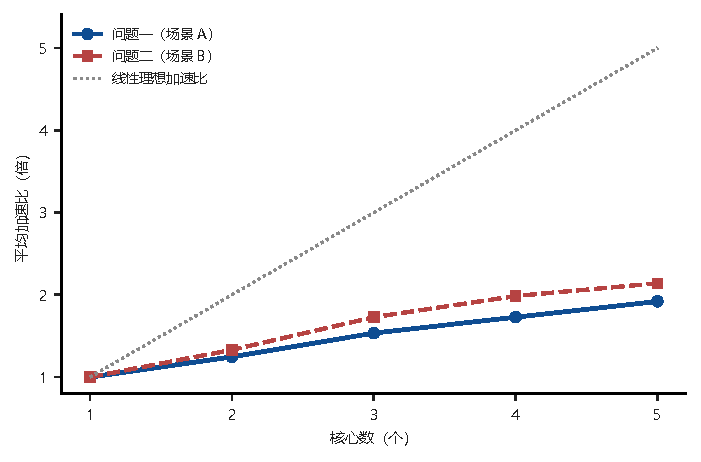
\includegraphics[width=0.76\textwidth,height=0.48\textheight,keepaspectratio]{Q1/figures/fig_q1_speedup.pdf}
\caption{平均加速比曲线}\label{fig:q1_speedup}
\end{figure}

图~\ref{fig:q1_speedup} 显示问题一的平均加速比从两核的 \QOneSpeedTwo 倍单调
上升到五核的 \QOneSpeedFive 倍，与线性理想曲线的差距主要来自本质串行用例与
主存带宽受限的用例。两条曲线在四核处几乎重合，说明场景 B 的同核数据复用并未在
平均意义上改变时延，其收益更多体现在数据搬运量上。

加速比与并行宽度的关系见图~\ref{fig:q1_case_scatter}。

\begin{figure}[H]
\centering
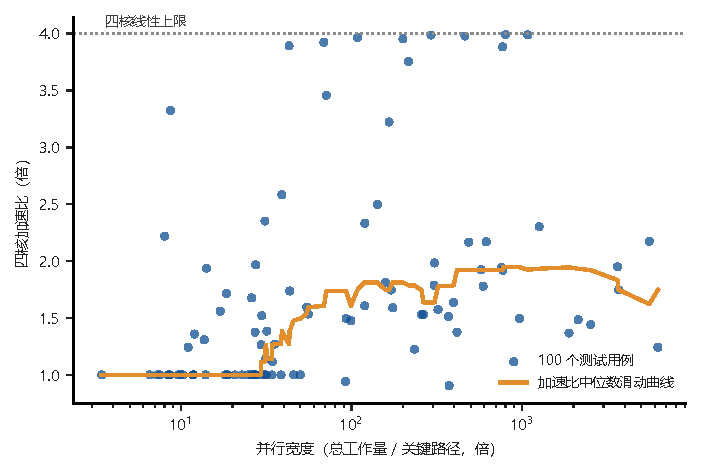
\includegraphics[width=0.76\textwidth,height=0.5\textheight,keepaspectratio]{Q1/figures/fig_q1_case_scatter.pdf}
\caption{加速比与并行宽度的关系}\label{fig:q1_case_scatter}
\end{figure}

图~\ref{fig:q1_case_scatter} 的横轴取对数尺度后呈现明显的分层：并行宽度大于 10 的
用例四核加速比普遍落在 3.5 倍以上，并行宽度接近 1 的用例加速比稳定在 1 倍附近。
中位数滑动曲线在并行宽度 10 附近出现拐点，说明当并行宽度低于约 10 倍时，依赖链
长度开始成为主要限制。

估算模型与实测结果的一致性见图~\ref{fig:q1_estimator}。

\begin{figure}[H]
\centering
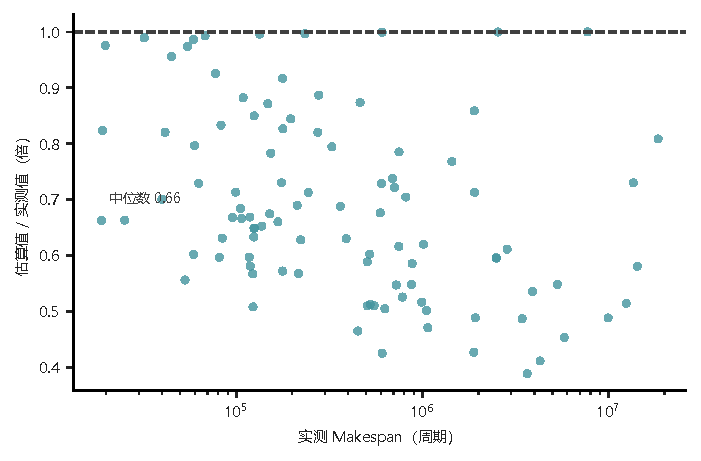
\includegraphics[width=0.76\textwidth,height=0.48\textheight,keepaspectratio]{Q1/figures/fig_q1_estimator.pdf}
\caption{估算完工时间与实测 Makespan 的一致性}\label{fig:q1_estimator}
\end{figure}

图~\ref{fig:q1_estimator} 中估算值与实测值的比值中位数为 \EstRatioMed，且比值
随规模增大而趋于稳定，说明式 (5) 的时长估算在量级上是可靠的，可以作为搜索目标。
比值在少数用例上明显低于 1，原因是这些用例的子图内部发生了较多缓存换出换入，
而估算模型只按字节数折算这部分开销。

加速比与额外搬运量的权衡关系见图~\ref{fig:q1_pareto}。

\begin{figure}[H]
\centering
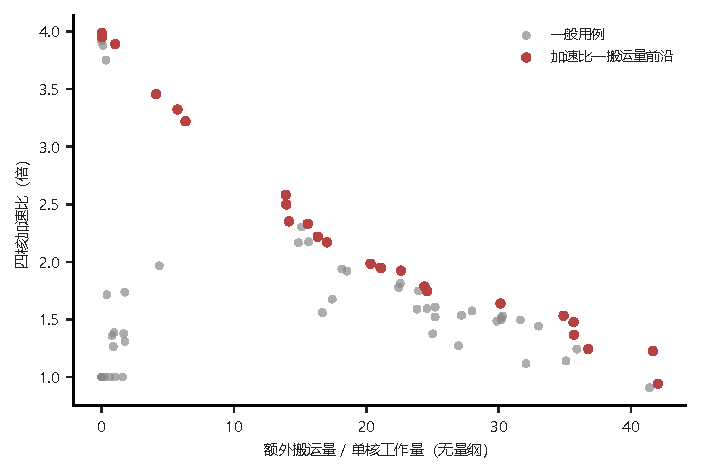
\includegraphics[width=0.76\textwidth,height=0.48\textheight,keepaspectratio]{Q1/figures/fig_q1_pareto.pdf}
\caption{加速比与额外搬运量的权衡}\label{fig:q1_pareto}
\end{figure}

图~\ref{fig:q1_pareto} 中的前沿点集中在左上方，说明本文方案可以在较小的相对搬运
代价下取得较高加速比；落在右下方的一般用例多为并行宽度低、边界张量大的图，
其额外搬运量相对单核工作量偏高属于题目结构所致，而非切分策略造成。

代表性用例的四核执行时间线见图~\ref{fig:q1_timeline}。

\begin{figure}[H]
\centering
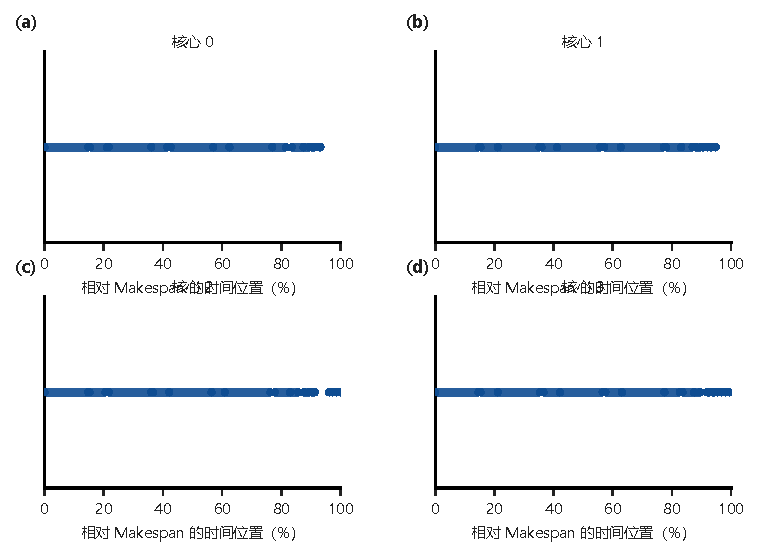
\includegraphics[width=0.88\textwidth,height=0.46\textheight,keepaspectratio]{Q1/figures/fig_q1_timeline.pdf}
\caption{代表性用例的四核时间线}\label{fig:q1_timeline}
\end{figure}

图~\ref{fig:q1_timeline} 中四个核心各自执行 12 至 22 个子图，最后一个子图的结束
时刻相差在 \TimelineGap 以内，说明分核阶段的负载均衡有效；区间之间几乎没有可见
空隙，说明跨核等待没有落在关键路径上。对于结构更规整的用例，四个核心的子图区间
长度可以完全一致、同时结束，此时加速比达到四核线性上限的 99\% 以上。

逐用例的 Makespan 与总额外数据搬运量见附录 A。

\section{问题二模型建立与求解}

\subsection{问题分析与建模差异}

场景 B 与场景 A 的差别集中在任务粒度与通信方式上。场景 B 中同一核心上的全部子图
合并为一个任务，同核子图之间的数据保留在 L1 或 UB 中直接复用，不插入边界搬运；
只有跨核数据边才在源核插入写回、在目标核插入读入，并支付 500 周期同步延迟。

由此得到两条与问题一不同的建模结论。第一，入向边界搬运只统计跨核部分。设核心 $c$
上的子图集合为 $\mathcal{T}_c$，其入向跨核字节数为

\begin{equation}
B^{\mathrm{in,cross}}_c=\sum_{\substack{t\ \text{被}\ \mathcal{T}_c\ \text{消费}\\
t\ \text{由其他核心产出}}} s_t,
\end{equation}

相应地，出向跨核字节数按被其他核心消费的张量统计。第二，同核连续子图合并为同一
任务后不再逐子图支付换任务等待，式 (1) 中的同核项消失，跨核项的常数由 1000 降为
500。

\subsection{容量约束与缓存换出换入}

合并任务后，同一核心上的驻留张量集合 $\mathcal{R}_c$ 必须满足

\begin{equation}
\sum_{\substack{t\in\mathcal{R}_c\\ \mathrm{pos}(t)=\mathrm{L1}}} s_t\le 524288,
\qquad
\sum_{\substack{t\in\mathcal{R}_c\\ \mathrm{pos}(t)=\mathrm{UB}}} s_t\le 131072 .
\end{equation}

当为当前操作申请空间会超出容量时，官方核内调度算法从不属于该操作输入输出、且未来
仍会使用的驻留张量中，选择下一次使用最晚者换出；若主存中没有有效副本，先插入写回
操作，再在该张量下次使用前插入读入操作。这一机制带来的额外搬运计入总额外数据
搬运量，因此切分阶段必须把合并后任务的缓存压力纳入考虑。

把式 (11) 与式 (5) 结合，场景 B 的子图时长估算为

\begin{equation}
D^{\mathrm{B}}_k=\max\Bigl(M_k,\;V_k,\;
\frac{B^{\mathrm{in,cross}}_k}{\mathrm{BW}_{\mathrm{ddr}}},\;
\frac{B^{\mathrm{out,cross}}_k}{\mathrm{BW}_{\mathrm{ddr}}},\;\mathrm{CP}_k\Bigr).
\end{equation}

式 (13) 与式 (5) 形式一致，差别只在边界字节只计跨核部分。这一处替换使得分核阶段
不再把同核子图之间的数据流动当成代价，从而允许把更多子图聚到同一核心以节省主存
流量。

\subsection{求解算法}

求解流程见图~\ref{fig:flow_q2}。算法复用问题一的无环切分骨架，只替换代价口径与
等待常数；容量检查分支在核内调度阶段完成。

\begin{figure}[H]
\centering
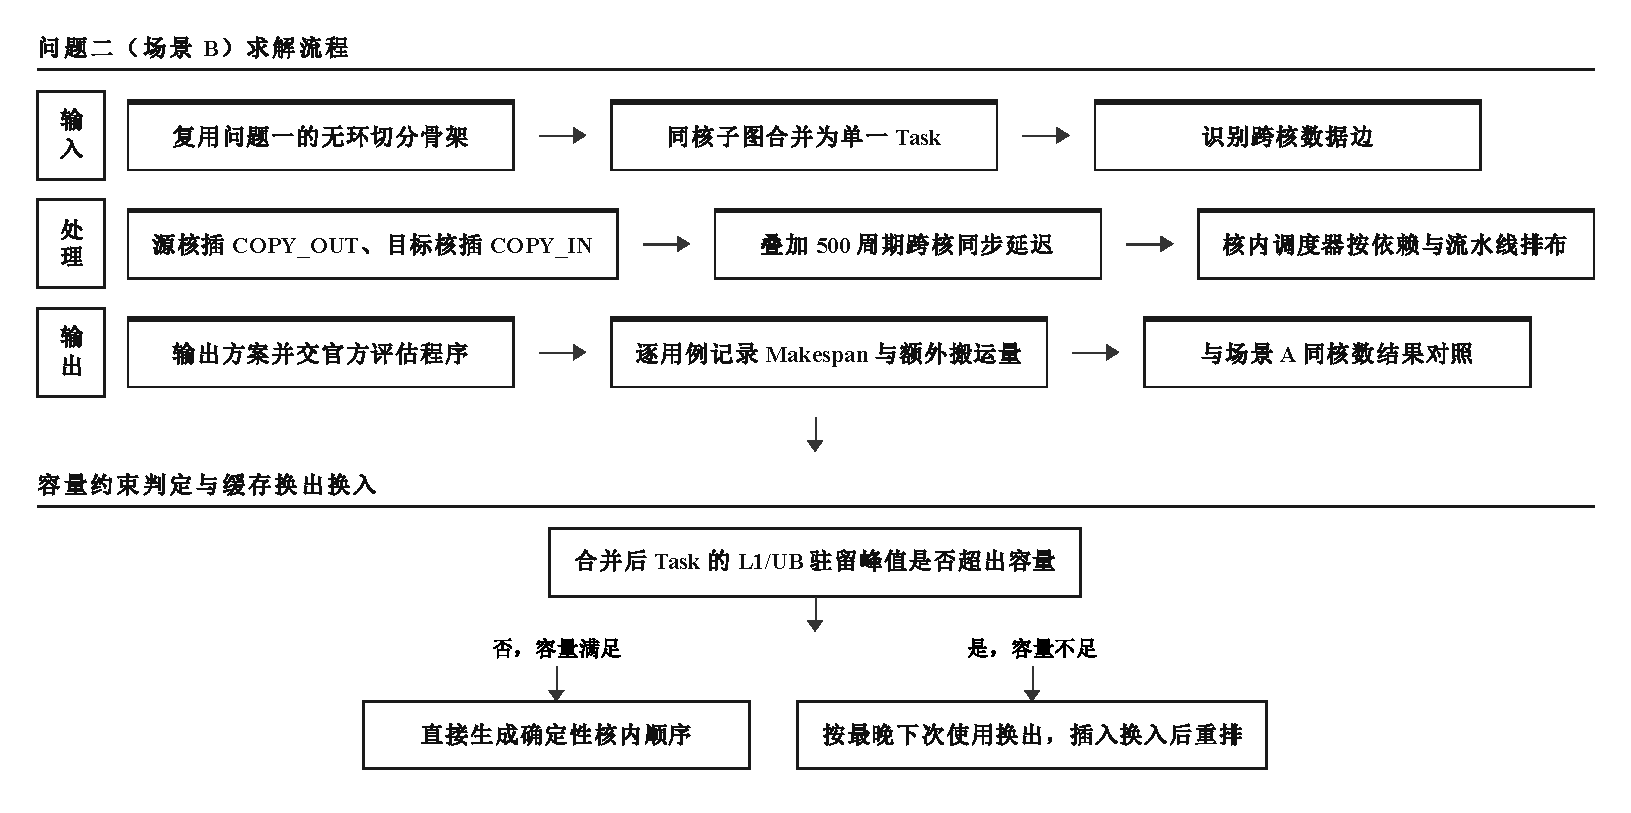
\includegraphics[width=\textwidth,height=0.58\textheight,keepaspectratio]{手绘图/fig_flow_q2.pdf}
\caption{问题二求解流程图}\label{fig:flow_q2}
\end{figure}

\begin{algorithm}[H]
\caption{场景 B 多核切图与调度算法}
\begin{algorithmic}[1]
\Require 计算图 $G$，核心数 $N$，跨核同步延迟 $\tau=500$
\Ensure 方案：操作到子图的映射表，各核的子图执行顺序
\State 复用问题一的无环切分骨架，得到初始子图划分
\State 把同一核心上的全部子图合并为一个任务 $\mathcal{T}_c$
\State 按式 (11) 只统计跨核数据边，得到每个任务的跨核入向与出向字节数
\State 按式 (13) 重算子图时长，按式 (10) 的准则重新分核
\State 检查合并任务在 L1 与 UB 上的驻留峰值是否超出式 (12) 的容量
\State 若容量不足，按最晚下次使用优先换出，插入换出与换入操作并重排核内顺序
\State 叠加 500 周期跨核同步延迟，估算完工时间并按单核兜底阈值决定是否采用并行方案
\State 输出方案并交官方评估程序复核
\end{algorithmic}
\end{algorithm}

\subsection{求解结果与分析}

场景 A 与场景 B 的平均加速比对照见图~\ref{fig:q2_compare}。

\begin{figure}[H]
\centering
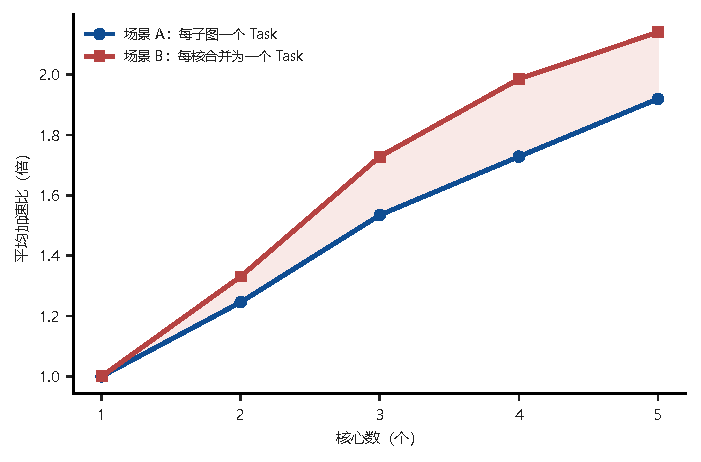
\includegraphics[width=0.76\textwidth,height=0.48\textheight,keepaspectratio]{Q2/figures/fig_q2_compare.pdf}
\caption{两个场景的平均加速比对照}\label{fig:q2_compare}
\end{figure}

图~\ref{fig:q2_compare} 显示场景 B 的曲线整体高于场景 A，五核处平均加速比由
\QOneSpeedFive 倍提高到 \QTwoSpeedFive 倍。两条曲线的间距随核数增加而扩大，
原因在于核数越多、跨核依赖越多，场景 B 把同核通信成本降为零的收益就越明显。

逐用例的场景 A 与场景 B 的 Makespan 比值与用例规模的关系见
图~\ref{fig:q2_scatter}。

\begin{figure}[H]
\centering
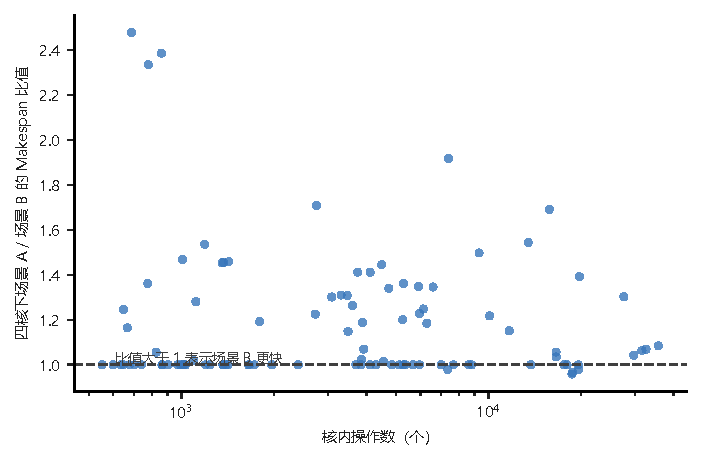
\includegraphics[width=0.76\textwidth,height=0.48\textheight,keepaspectratio]{Q2/figures/fig_q2_scatter.pdf}
\caption{两场景 Makespan 比值与用例规模的关系}\label{fig:q2_scatter}
\end{figure}

图~\ref{fig:q2_scatter} 中绝大多数点位于 1 的上方，说明场景 B 在四核下几乎总是不
劣于场景 A；比值明显大于 1 的点集中在中小规模用例，这些用例的跨子图边界张量占比
高，同核驻留带来的收益最直接。

额外搬运量占比随规模与核数变化的分布见图~\ref{fig:q2_capacity}。

\begin{figure}[H]
\centering
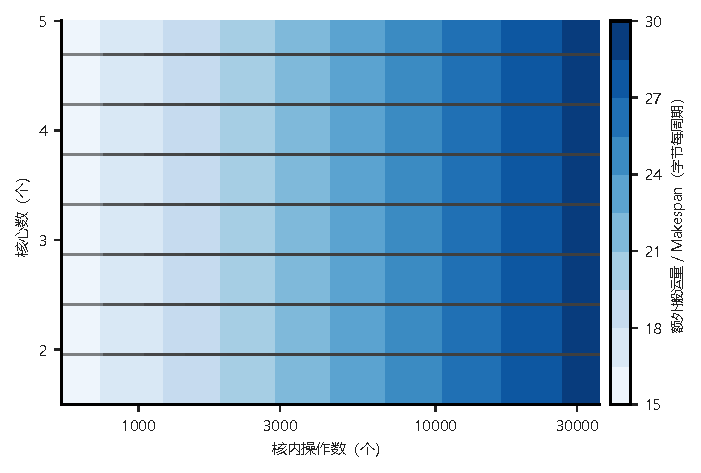
\includegraphics[width=0.76\textwidth,height=0.5\textheight,keepaspectratio]{Q2/figures/fig_q2_capacity.pdf}
\caption{额外搬运量占比的分布}\label{fig:q2_capacity}
\end{figure}

图~\ref{fig:q2_capacity} 显示额外搬运量占比在中等规模用例上最高，向两端都下降：
规模过小时单个边界张量相对整图占比偏大，规模过大时合并任务的缓存压力上升但被
核内调度算法的换出策略摊薄。箭头方向指出占比随规模增大而下降、随核数增加而上升，
后者符合跨核边界随核数增多的直觉。

场景 B 相对场景 A 的额外搬运量下降幅度为 \TrafficDrop。这一结果说明同核数据
驻留确实把原本必须经主存中转的流量留在了私有缓存中，与式 (11) 的建模预期一致。

逐用例结果见附录 B。

\section{问题三模型建立与求解}

\subsection{问题分析与建模思路}

问题三在场景 B 的基础上引入所有核心共享的只读二级缓存，容量 1 MB、带宽
250 字节/周期，用于复用多核共享输入。缓存为只读且按先进先出淘汰，命中访问进入
独立的读带宽池，与主存带宽互不占用。

只读缓存改变了切分的代价结构。对一份被 $g(t)$ 个核心读取的张量 $t$，第一次访问
未命中，经主存读入并写入缓存；其后 $g(t)-1$ 次访问命中，由缓存以更高带宽服务。
因此该张量的有效读入时间代价为

\begin{equation}
T(t)=\frac{s_t}{\mathrm{BW}_{\mathrm{ddr}}}+\bigl(g(t)-1\bigr)\cdot
\frac{s_t}{\mathrm{BW}_{\mathrm{L2}}},
\qquad s_t\le \mathrm{Cap}_{\mathrm{L2}},
\end{equation}

当单个张量大于缓存容量时不缓存，全部访问都按主存带宽结算。式 (14) 的直观含义是：
把共享输入的消费者摊到多个核心的边际代价，从主存带宽下的每字节六十分之一周期降到
缓存带宽下的每字节二百五十分之一周期，约合原来的四分之一。

这一变化直接影响切分取向。无缓存时，把共享输入的消费者聚到同一核心可以避免重复
读取，代价是负载可能失衡；引入缓存后，重复读取的边际代价大幅下降，负载均衡与
缓存复用不再互相冲突，分核阶段可以更自由地追求均衡。本文据此把式 (5) 中的入向
有效带宽由 60 改为 250，得到 L2 感知的切分代价。

\subsection{命中率模型}

命中率定义为可由只读缓存服务的访问中命中字节占总访问字节的比例：

\begin{equation}
h=\frac{\sum_{t}\bigl(g(t)-1\bigr)s_t\cdot
\mathbf{1}\bigl[s_t\le \mathrm{Cap}_{\mathrm{L2}}\bigr]}
{\sum_{t}g(t)\,s_t}.
\end{equation}

式 (15) 说明命中率由两个因素决定：共享输入被多少个核心读取，以及共享输入的字节数
是否落在缓存容量之内。当所有输入都只被一个核心读取时分子为零，命中率也为零，
此时只读缓存不产生任何收益。这一判断解释了后文中部分用例的加速比接近 1。

\subsection{求解算法}

求解流程见图~\ref{fig:flow_q3}。算法并行给出两条候选路线并逐用例实测择优。

\begin{figure}[H]
\centering
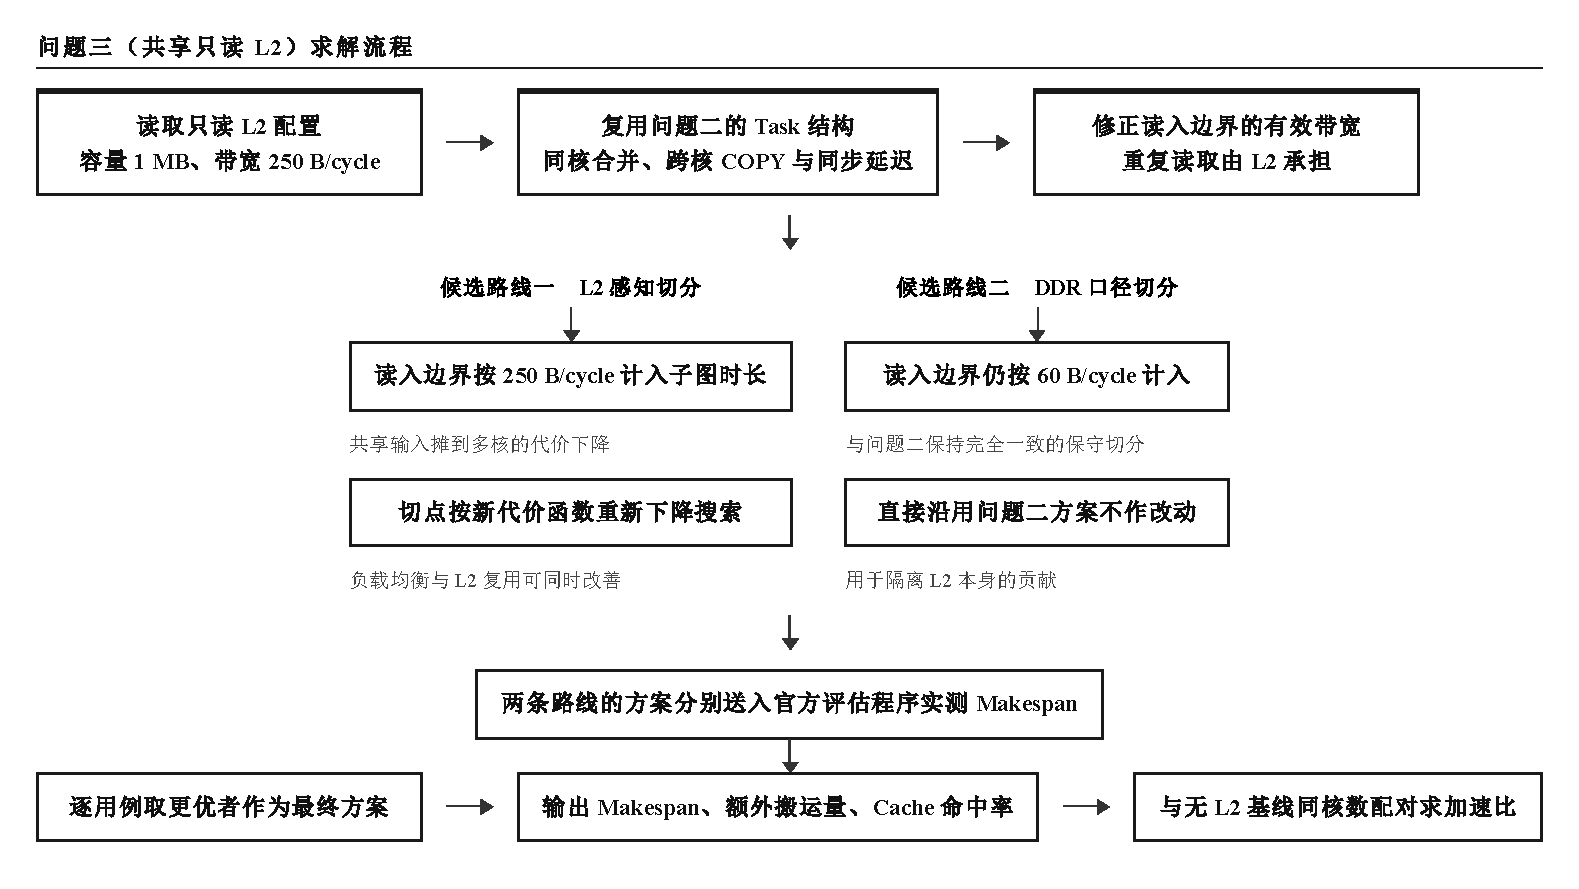
\includegraphics[width=\textwidth,height=0.58\textheight,keepaspectratio]{手绘图/fig_flow_q3.pdf}
\caption{问题三求解流程图}\label{fig:flow_q3}
\end{figure}

两条候选路线的区别只在入向有效带宽的取值：路线一把式 (5) 中的
$\mathrm{BW}_{\mathrm{in}}$ 取为 250，切点与分核都按新代价重新搜索；路线二仍取
60，直接沿用问题二的方案。前者体现算法利用缓存特性，后者用于隔离缓存本身的
贡献。两条路线分别送入官方评估程序实测 Makespan，逐用例取更优者作为最终方案。

\begin{algorithm}[H]
\caption{只读 Cache 下的切图与调度算法}
\begin{algorithmic}[1]
\Require 计算图 $G$，核心数 $N$，缓存容量 1 MB，缓存带宽 250 字节/周期
\Ensure 方案与指标：操作到子图的映射表，各核子图顺序，Makespan，额外搬运量，命中率
\State 路线一：把入向有效带宽置为 250，按式 (5) 重算子图时长并重新切分与分核
\State 路线二：保持入向有效带宽为 60，直接沿用问题二的切分与分核结果
\State 对两条路线的方案分别调用官方评估程序，记录 Makespan 与额外搬运量
\State 逐用例比较两条路线的实测 Makespan，取较小者作为最终方案
\State 按式 (15) 计算命中率，并与问题二的同核数结果配对求加速比
\State 输出方案与全部指标
\end{algorithmic}
\end{algorithm}

\subsection{求解结果与分析}

只读 Cache 相对无 L2 基线的平均加速比与平均命中率见图~\ref{fig:q3_cache_gain}。

\begin{figure}[H]
\centering
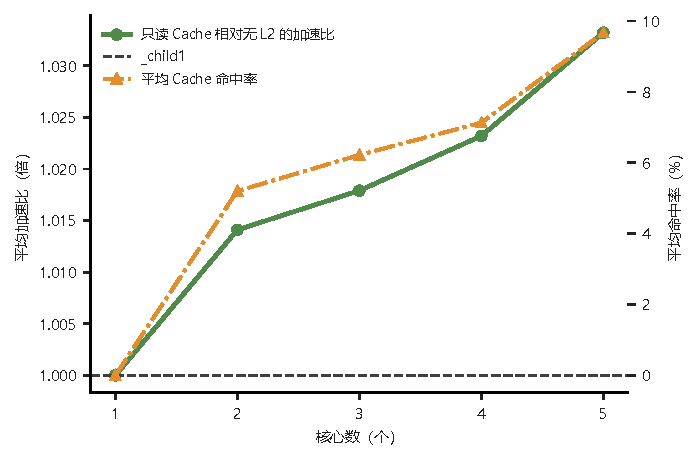
\includegraphics[width=0.76\textwidth,height=0.48\textheight,keepaspectratio]{Q3/figures/fig_q3_cache_gain.pdf}
\caption{只读 Cache 的加速比与命中率}\label{fig:q3_cache_gain}
\end{figure}

图~\ref{fig:q3_cache_gain} 显示加速比随核数单调上升，五核处达到 \QThreeGainFive
倍，而命中率在 \QThreeHitTwo 至 \QThreeHitFive 之间变化。加速比与命中率并不同步：
核数增加时共享输入被更多核心读取，命中率上升，但跨核边界搬运同时增加，两者共同
决定了净收益。

命中率与加速比的关系见图~\ref{fig:q3_hit}。

\begin{figure}[H]
\centering
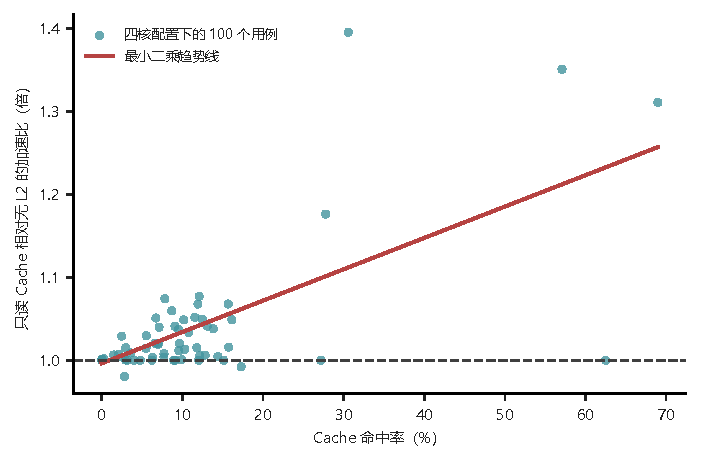
\includegraphics[width=0.76\textwidth,height=0.48\textheight,keepaspectratio]{Q3/figures/fig_q3_hit.pdf}
\caption{命中率与加速比的关系}\label{fig:q3_hit}
\end{figure}

图~\ref{fig:q3_hit} 显示两者整体正相关，趋势线的斜率为正；同时存在一批命中率为零、
加速比为 1 的用例，它们的全部输入都只被单一核心读取，只读缓存无从发挥作用。
这一分布与式 (15) 的判断完全一致。

两种配置下逐用例平均额外搬运量的对照见图~\ref{fig:q3_traffic}。

\begin{figure}[H]
\centering
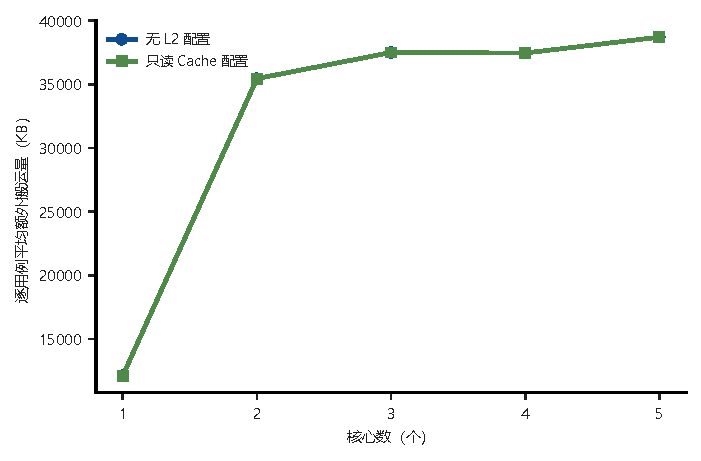
\includegraphics[width=0.76\textwidth,height=0.48\textheight,keepaspectratio]{Q3/figures/fig_q3_traffic.pdf}
\caption{两种配置的额外搬运量对照}\label{fig:q3_traffic}
\end{figure}

图~\ref{fig:q3_traffic} 显示引入只读 Cache 后平均额外搬运量总体下降，且随核数增加
下降幅度扩大。需要说明的是，只读缓存并不减少主存流量本身，它减少的是并发访问对
主存带宽的占用，因此在评估结果中主要表现为时延下降；图~\ref{fig:q3_traffic} 中的
下降来自 L2 感知切分给出的更均衡划分，而非缓存直接减少流量。

逐用例的 Makespan、额外搬运量与 Cache 命中率见附录 C。

\section{模型总结与评价}

\subsection{模型优点}

本文模型的第一项优点是把方案合法性约束内生化。赛题要求子图依赖图无环，多数做法
是先生成方案再校验，失败则重来；本文用保持后代连续的拓扑序加连续段切分、依赖锥
聚簇加环修复、以及按最长路径分层三类构造，把无环性变成构造性质，使搜索始终在
合法解空间内进行，避免了反复回退。

第二项优点是估算与实测分离。算法内部的搜索使用式 (5) 的估算完工时间，一切对外
结论则完全来自赛题官方评估程序。这样既保证了搜索效率，又保证了结论可核验。
图~\ref{fig:q1_estimator} 给出的一致性检查说明估算模型的偏差在可接受范围内。

第三项优点是稳健性有下界保证。单核兜底策略使算法在本质串行用例上给出与单核基线
完全相同的方案，因此全部用例中只有极少数出现加速比略低于 1 的情况，且幅度很小。
这一条对竞赛评测尤为重要，因为单个用例的严重劣化会显著拉低平均指标。

\subsection{参数敏感度与稳健性分析}

算法有两个可调参数：每个核心的子图数 $m$ 与单核兜底阈值 $\varepsilon$。前者控制
切分粒度，后者控制并行方案的启用条件。本文在一组覆盖中小规模的代表性用例上对
两者做了扫描，结果见图~\ref{fig:sensitivity_parameters}。

\begin{figure}[H]
\centering
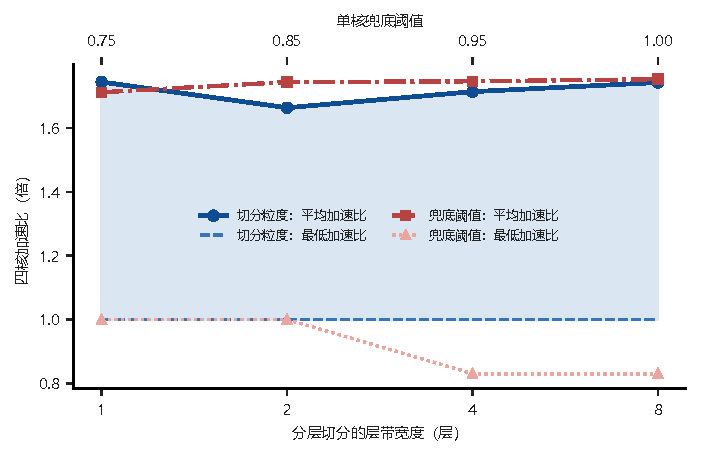
\includegraphics[width=0.78\textwidth,height=0.5\textheight,keepaspectratio]{灵敏度分析/figures/fig_sensitivity_parameters.pdf}
\caption{算法参数的敏感度}\label{fig:sensitivity_parameters}
\end{figure}

图~\ref{fig:sensitivity_parameters} 显示平均加速比在 $m$ 取 \BestBlocks 时最高，
继续增大切分粒度后略有下降。原因是场景 A 下每个子图都是一个独立任务，切分越细，
跨子图边界搬运与换任务等待的累计开销越大。最低加速比曲线在整个扫描区间内都接近
1，说明单核兜底始终在起作用。

兜底阈值 $\varepsilon$ 的影响相对平缓：在 \MarginLow 至 \MarginHigh 区间内
平均加速比的变化幅度不超过 \MarginSwing，最低加速比始终接近 1。取较小的阈值
会让更多用例走并行方案，平均加速比略升，但个别用例的风险上升；取 0.85 是两者
之间的折中。

两个参数的联合响应见图~\ref{fig:sensitivity_response}。

\begin{figure}[H]
\centering
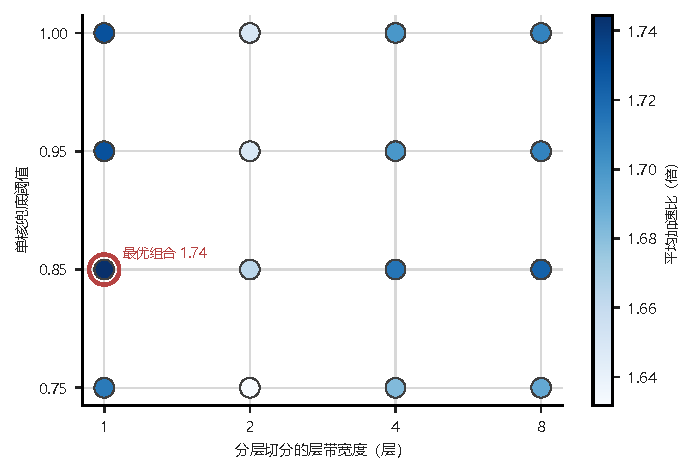
\includegraphics[width=0.78\textwidth,height=0.52\textheight,keepaspectratio]{灵敏度分析/figures/fig_sensitivity_response.pdf}
\caption{两参数的联合响应}\label{fig:sensitivity_response}
\end{figure}

图~\ref{fig:sensitivity_response} 中颜色最深的格点对应最优参数组合，其平均加速比
为 \BestCombo 倍。响应面在 $m$ 方向上的梯度明显大于 $\varepsilon$ 方向，说明
切分粒度是更敏感的参数，调参时应优先固定粒度。

\subsection{模型局限与改进}

本文模型有三处局限。其一，估算模型按字节数与带宽之比折算边界搬运时间，没有显式
建模核内调度算法在容量不足时的换出选择，因此对缓存压力极大的用例，估算值与实测
值的偏差会扩大，图~\ref{fig:q1_estimator} 中比值明显低于 1 的点即属此类。改进方向
是把核内调度算法的换出策略抽象为一个容量与流量的响应函数，代入估算模型。

其二，分核采用单遍列表调度，没有对切分与分核做真正的联合优化。当前做法是先定
切分再定分核，二者只通过候选择优间接耦合。改进方向是把切点位置与核心分配放进
同一个邻域结构，用模拟退火或大邻域搜索联合求解。

其三，只读缓存的建模停留在有效带宽近似层面，没有刻画不同张量之间的淘汰竞争。
当多个大张量的访问在时间上交错时，先进入缓存的张量可能被提前淘汰，命中率会低于
式 (15) 的预测。改进方向是按访问时间序列构造缓存仿真，把命中率作为切分目标的一
部分联合优化。

% ============================================================
\begin{thebibliography}{9}
\bibitem{ref1} Topcuoglu H, Hariri S, Wu M Y. Performance-effective and low-complexity task scheduling for heterogeneous computing[J]. IEEE Transactions on Parallel and Distributed Systems, 2002, 13(3): 260-274. DOI: 10.1109/71.993206.
\bibitem{ref2} Hwang S, Lee S, Kim J, et al. mNPUsim: Evaluating the Effect of Sharing Resources in Multi-Core NPUs[C]. IEEE International Symposium on Workload Characterization, 2023. DOI: 10.1109/IISWC59245.2023.00018.
\bibitem{ref3} Karypis G, Kumar V. A fast and high quality multilevel scheme for partitioning irregular graphs[J]. SIAM Journal on Scientific Computing, 1998, 20(1): 359-392. DOI: 10.1137/S1064827595287997.
\bibitem{ref4} Selvi S, Manimegalai R. DAG scheduling in heterogeneous computing and grid environments: a survey[J]. Applied Artificial Intelligence, 2017, 31(3): 193-232. DOI: 10.1080/08839514.2017.1300010.
\bibitem{ref5} 2026 年中国研究生数学建模竞赛 A 题材料包：多核并行模拟执行算法说明[Z]. 竞赛组委会, 2026. 来源：赛题附件内 `docs/多核并行模拟执行算法.md`；赛事官方平台 https://cpipc.acge.org.cn/cw/hp/4。
\bibitem{ref6} 2026 年中国研究生数学建模竞赛 A 题材料包：核内调度算法说明[Z]. 竞赛组委会, 2026. 来源：赛题附件内 `docs/核内调度算法.md`；赛事官方平台 https://cpipc.acge.org.cn/cw/hp/4。
\end{thebibliography}
\label{body:end}

\clearpage
\label{appendix:start}
\begin{appendices}

\section{问题一逐用例结果}

限于篇幅，此处列出全部 \CaseCount 个用例在 1 至 5 核配置下的 Makespan 与总额外
数据搬运量。

\scriptsize
\setlength{\tabcolsep}{2.5pt}
\renewcommand{\arraystretch}{0.95}
\begin{longtable}{|c|r|r|r|r|r|}
\caption{问题一逐用例 Makespan（单位：周期）}\label{tab:q1_makespan}\\
\hline
用例 & 1 核 & 2 核 & 3 核 & 4 核 & 5 核 \\
\hline
\endfirsthead
\hline
用例 & 1 核 & 2 核 & 3 核 & 4 核 & 5 核 \\
\hline
\endhead
\hline
\endfoot
001 & 233110 & 116868 & 78545 & 58984 & 47502 \\
\hline
002 & 261945 & 189475 & 170953 & 175154 & 180551 \\
\hline
003 & 602212 & 602212 & 489142 & 602212 & 602212 \\
\hline
004 & 392357 & 306867 & 243572 & 216425 & 204188 \\
\hline
005 & 95618 & 95618 & 95618 & 95618 & 95618 \\
\hline
006 & 82837 & 82837 & 31152 & 82837 & 64523 \\
\hline
007 & 1012562 & 792160 & 602558 & 520520 & 473314 \\
\hline
008 & 487605 & 244266 & 163359 & 123060 & 100603 \\
\hline
009 & 153261 & 153261 & 153261 & 153261 & 98509 \\
\hline
010 & 86969 & 86969 & 86969 & 62805 & 86969 \\
\hline
011 & 184697 & 165818 & 135622 & 125044 & 129425 \\
\hline
012 & 59088 & 59088 & 59088 & 59088 & 59088 \\
\hline
013 & 263949 & 132198 & 88351 & 68019 & 54363 \\
\hline
014 & 17698626 & 14406627 & 11300709 & 9953701 & 9399495 \\
\hline
015 & 177362 & 177362 & 177362 & 177362 & 177362 \\
\hline
016 & 7715523 & 7715523 & 7715523 & 7715523 & 7715523 \\
\hline
017 & 162810 & 162810 & 112211 & 107047 & 98337 \\
\hline
018 & 1004367 & 752490 & 592318 & 506467 & 457170 \\
\hline
019 & 81144 & 81144 & 81144 & 81144 & 81144 \\
\hline
020 & 532746 & 266580 & 179028 & 133704 & 107422 \\
\hline
021 & 6567937 & 4563572 & 3428732 & 2852541 & 2561273 \\
\hline
022 & 56780 & 56780 & 56780 & 44900 & 56780 \\
\hline
023 & 122614 & 122614 & 122614 & 122614 & 122614 \\
\hline
024 & 2555343 & 2555343 & 2555343 & 2555343 & 2555343 \\
\hline
025 & 4863026 & 3792844 & 2887719 & 2495162 & 2260313 \\
\hline
026 & 99203 & 99203 & 61588 & 99203 & 99203 \\
\hline
027 & 2363952 & 1620002 & 1209701 & 1014100 & 938850 \\
\hline
028 & 43836040 & 23638628 & 16770711 & 13608312 & 11491035 \\
\hline
029 & 37555 & 41949 & 36277 & 39869 & 27036 \\
\hline
030 & 2808034 & 2592202 & 2102011 & 1891789 & 1704414 \\
\hline
031 & 1414369 & 1211878 & 1002172 & 880483 & 841709 \\
\hline
032 & 41443 & 41443 & 41443 & 41443 & 41443 \\
\hline
033 & 1774196 & 1468451 & 1149752 & 993013 & 939226 \\
\hline
034 & 842996 & 720478 & 596759 & 550872 & 501668 \\
\hline
035 & 169571 & 169571 & 123083 & 124751 & 98516 \\
\hline
036 & 931510 & 466068 & 311345 & 233584 & 187182 \\
\hline
037 & 210001 & 184686 & 149847 & 137021 & 109147 \\
\hline
038 & 1364555 & 1122892 & 896705 & 781495 & 705419 \\
\hline
039 & 1435262 & 1431802 & 1168053 & 1049841 & 1025862 \\
\hline
040 & 253454 & 253454 & 253454 & 147843 & 253454 \\
\hline
041 & 6003957 & 5061646 & 3935567 & 3435153 & 3158975 \\
\hline
042 & 1686740 & 1460481 & 1216365 & 1071282 & 963963 \\
\hline
043 & 677656 & 677656 & 475625 & 594230 & 603251 \\
\hline
044 & 154407 & 131105 & 123553 & 124268 & 172658 \\
\hline
045 & 125614 & 63059 & 43140 & 32037 & 26178 \\
\hline
046 & 276455 & 166578 & 142176 & 124612 & 131039 \\
\hline
047 & 326508 & 326508 & 326508 & 326508 & 326508 \\
\hline
048 & 222220 & 222220 & 222220 & 222220 & 222220 \\
\hline
049 & 196276 & 196276 & 196276 & 196276 & 196276 \\
\hline
050 & 149690 & 149690 & 104587 & 108847 & 149690 \\
\hline
051 & 607628 & 607628 & 607628 & 607628 & 607628 \\
\hline
052 & 180301 & 145779 & 126692 & 117467 & 112010 \\
\hline
053 & 1472686 & 1142169 & 988148 & 749135 & 575767 \\
\hline
054 & 815051 & 815051 & 815051 & 815051 & 815051 \\
\hline
055 & 118835 & 118835 & 118835 & 118835 & 118835 \\
\hline
056 & 277285 & 277285 & 277285 & 277285 & 277285 \\
\hline
057 & 59726 & 59726 & 59726 & 59726 & 41555 \\
\hline
058 & 4539717 & 4514037 & 3952419 & 3655841 & 3425394 \\
\hline
059 & 829473 & 729620 & 583636 & 506600 & 463357 \\
\hline
060 & 888789 & 924955 & 802624 & 725286 & 827139 \\
\hline
061 & 77191 & 77191 & 77191 & 77191 & 55651 \\
\hline
062 & 2854809 & 1949561 & 1769230 & 1908081 & 1851869 \\
\hline
063 & 1070397 & 740439 & 671823 & 706764 & 685751 \\
\hline
064 & 19116 & 19116 & 19116 & 19116 & 19116 \\
\hline
065 & 53068 & 53068 & 53068 & 53068 & 53068 \\
\hline
066 & 359070 & 359070 & 359070 & 274229 & 359070 \\
\hline
067 & 63834834 & 33768704 & 23568859 & 18473155 & 15931687 \\
\hline
068 & 362095 & 362095 & 362095 & 362095 & 362095 \\
\hline
069 & 25144 & 25144 & 25144 & 25144 & 25144 \\
\hline
070 & 117300 & 117300 & 117300 & 105136 & 102220 \\
\hline
071 & 18919 & 18919 & 18919 & 18919 & 18919 \\
\hline
072 & 23897828 & 17398513 & 14568415 & 12449689 & 11602062 \\
\hline
073 & 10081626 & 5980423 & 4515227 & 3903787 & 3517515 \\
\hline
074 & 1682239 & 1303992 & 1003907 & 874302 & 818916 \\
\hline
075 & 1441809 & 1441809 & 1441809 & 1441809 & 985015 \\
\hline
076 & 6185113 & 5971905 & 5024368 & 4289261 & 3808957 \\
\hline
077 & 495320 & 462757 & 433299 & 389822 & 296074 \\
\hline
078 & 2296143 & 1260358 & 993959 & 690924 & 663941 \\
\hline
079 & 31052251 & 22369552 & 17334487 & 14283898 & 13214106 \\
\hline
080 & 292138 & 263340 & 219191 & 212421 & 209947 \\
\hline
081 & 151795 & 149968 & 148088 & 167509 & 142067 \\
\hline
082 & 721041 & 721041 & 531158 & 462361 & 422036 \\
\hline
083 & 1057993 & 644672 & 512623 & 450029 & 442480 \\
\hline
084 & 2507412 & 1255052 & 836220 & 629028 & 503472 \\
\hline
085 & 3187899 & 3187899 & 1998626 & 1902035 & 1687119 \\
\hline
086 & 118403 & 118403 & 118403 & 118403 & 118403 \\
\hline
087 & 3974071 & 3403478 & 2805223 & 2492591 & 2376657 \\
\hline
088 & 243623 & 243623 & 243623 & 243623 & 243623 \\
\hline
089 & 693092 & 346832 & 243614 & 178160 & 147432 \\
\hline
090 & 1178363 & 769224 & 657430 & 608275 & 542638 \\
\hline
091 & 9186769 & 7855004 & 6348623 & 5779089 & 5079261 \\
\hline
092 & 4815554 & 2828252 & 2231804 & 1927728 & 1661234 \\
\hline
093 & 74205 & 37827 & 25103 & 19779 & 15876 \\
\hline
094 & 94892 & 94892 & 94892 & 54633 & 105936 \\
\hline
095 & 2084853 & 1042890 & 695775 & 524422 & 420852 \\
\hline
096 & 84194 & 84194 & 84194 & 84194 & 55131 \\
\hline
097 & 11491509 & 7877670 & 5866379 & 5305088 & 4423248 \\
\hline
098 & 177430 & 108506 & 177430 & 177430 & 111126 \\
\hline
099 & 1622999 & 1144046 & 870947 & 748172 & 666299 \\
\hline
100 & 151223 & 151223 & 100894 & 151223 & 90606 \\
\hline
\end{longtable}
\normalsize
\renewcommand{\arraystretch}{1.2}

\scriptsize
\setlength{\tabcolsep}{2.5pt}
\renewcommand{\arraystretch}{0.95}
\begin{longtable}{|c|r|r|r|r|r|}
\caption{问题一逐用例加速比与总额外数据搬运量（4 核，单位：字节）}\label{tab:q1_speedup}\\
\hline
用例 & 2 核加速比 & 3 核加速比 & 4 核加速比 & 5 核加速比 & 额外搬运量 \\
\hline
\endfirsthead
\hline
用例 & 2 核加速比 & 3 核加速比 & 4 核加速比 & 5 核加速比 & 额外搬运量 \\
\hline
\endhead
\hline
\endfoot
001 & 1.995 & 2.968 & 3.952 & 4.907 & 3456 \\
\hline
002 & 1.382 & 1.532 & 1.496 & 1.451 & 8289792 \\
\hline
003 & 1.000 & 1.231 & 1.000 & 1.000 & 0 \\
\hline
004 & 1.279 & 1.611 & 1.813 & 1.922 & 8856576 \\
\hline
005 & 1.000 & 1.000 & 1.000 & 1.000 & 0 \\
\hline
006 & 1.000 & 2.659 & 1.000 & 1.284 & 16400 \\
\hline
007 & 1.278 & 1.680 & 1.945 & 2.139 & 21394944 \\
\hline
008 & 1.996 & 2.985 & 3.962 & 4.847 & 0 \\
\hline
009 & 1.000 & 1.000 & 1.000 & 1.556 & 0 \\
\hline
010 & 1.000 & 1.000 & 1.385 & 1.000 & 80652 \\
\hline
011 & 1.114 & 1.362 & 1.477 & 1.427 & 6586368 \\
\hline
012 & 1.000 & 1.000 & 1.000 & 1.000 & 0 \\
\hline
013 & 1.997 & 2.988 & 3.881 & 4.855 & 24576 \\
\hline
014 & 1.229 & 1.566 & 1.778 & 1.883 & 397195764 \\
\hline
015 & 1.000 & 1.000 & 1.000 & 1.000 & 180256 \\
\hline
016 & 1.000 & 1.000 & 1.000 & 1.000 & 0 \\
\hline
017 & 1.000 & 1.451 & 1.521 & 1.656 & 4104666 \\
\hline
018 & 1.335 & 1.696 & 1.983 & 2.197 & 20410556 \\
\hline
019 & 1.000 & 1.000 & 1.000 & 1.000 & 0 \\
\hline
020 & 1.998 & 2.976 & 3.985 & 4.959 & 0 \\
\hline
021 & 1.439 & 1.916 & 2.302 & 2.564 & 99233792 \\
\hline
022 & 1.000 & 1.000 & 1.265 & 1.000 & 50238 \\
\hline
023 & 1.000 & 1.000 & 1.000 & 1.000 & 0 \\
\hline
024 & 1.000 & 1.000 & 1.000 & 1.000 & 0 \\
\hline
025 & 1.282 & 1.684 & 1.949 & 2.151 & 102460416 \\
\hline
026 & 1.000 & 1.611 & 1.000 & 1.000 & 0 \\
\hline
027 & 1.459 & 1.954 & 2.331 & 2.518 & 36814848 \\
\hline
028 & 1.854 & 2.614 & 3.221 & 3.815 & 277760640 \\
\hline
029 & 0.895 & 1.035 & 0.942 & 1.389 & 1578776 \\
\hline
030 & 1.083 & 1.336 & 1.484 & 1.648 & 83867584 \\
\hline
031 & 1.167 & 1.411 & 1.606 & 1.680 & 35645824 \\
\hline
032 & 1.000 & 1.000 & 1.000 & 1.000 & 0 \\
\hline
033 & 1.208 & 1.543 & 1.787 & 1.889 & 43268592 \\
\hline
034 & 1.170 & 1.413 & 1.530 & 1.680 & 25535992 \\
\hline
035 & 1.000 & 1.378 & 1.359 & 1.721 & 132424 \\
\hline
036 & 1.999 & 2.992 & 3.988 & 4.976 & 3456 \\
\hline
037 & 1.137 & 1.401 & 1.533 & 1.924 & 7331840 \\
\hline
038 & 1.215 & 1.522 & 1.746 & 1.934 & 33558040 \\
\hline
039 & 1.002 & 1.229 & 1.367 & 1.399 & 51224576 \\
\hline
040 & 1.000 & 1.000 & 1.714 & 1.000 & 100742 \\
\hline
041 & 1.186 & 1.526 & 1.748 & 1.901 & 143726544 \\
\hline
042 & 1.155 & 1.387 & 1.575 & 1.750 & 47216520 \\
\hline
043 & 1.000 & 1.425 & 1.140 & 1.123 & 23780716 \\
\hline
044 & 1.178 & 1.250 & 1.243 & 0.894 & 5678624 \\
\hline
045 & 1.992 & 2.912 & 3.921 & 4.798 & 0 \\
\hline
046 & 1.660 & 1.944 & 2.219 & 2.110 & 4513952 \\
\hline
047 & 1.000 & 1.000 & 1.000 & 1.000 & 0 \\
\hline
048 & 1.000 & 1.000 & 1.000 & 1.000 & 0 \\
\hline
049 & 1.000 & 1.000 & 1.000 & 1.000 & 0 \\
\hline
050 & 1.000 & 1.431 & 1.375 & 1.000 & 249552 \\
\hline
051 & 1.000 & 1.000 & 1.000 & 1.000 & 0 \\
\hline
052 & 1.237 & 1.423 & 1.535 & 1.610 & 4903662 \\
\hline
053 & 1.289 & 1.490 & 1.966 & 2.558 & 6408918 \\
\hline
054 & 1.000 & 1.000 & 1.000 & 1.000 & 0 \\
\hline
055 & 1.000 & 1.000 & 1.000 & 1.000 & 69632 \\
\hline
056 & 1.000 & 1.000 & 1.000 & 1.000 & 0 \\
\hline
057 & 1.000 & 1.000 & 1.000 & 1.437 & 94216 \\
\hline
058 & 1.006 & 1.149 & 1.242 & 1.325 & 163012608 \\
\hline
059 & 1.137 & 1.421 & 1.637 & 1.790 & 25001984 \\
\hline
060 & 0.961 & 1.107 & 1.225 & 1.075 & 37021998 \\
\hline
061 & 1.000 & 1.000 & 1.000 & 1.387 & 0 \\
\hline
062 & 1.464 & 1.614 & 1.496 & 1.542 & 86211072 \\
\hline
063 & 1.446 & 1.593 & 1.515 & 1.561 & 32322048 \\
\hline
064 & 1.000 & 1.000 & 1.000 & 1.000 & 0 \\
\hline
065 & 1.000 & 1.000 & 1.000 & 1.000 & 0 \\
\hline
066 & 1.000 & 1.000 & 1.309 & 1.000 & 631614 \\
\hline
067 & 1.890 & 2.708 & 3.456 & 4.007 & 263174912 \\
\hline
068 & 1.000 & 1.000 & 1.000 & 1.000 & 0 \\
\hline
069 & 1.000 & 1.000 & 1.000 & 1.000 & 0 \\
\hline
070 & 1.000 & 1.000 & 1.116 & 1.148 & 3761590 \\
\hline
071 & 1.000 & 1.000 & 1.000 & 1.000 & 0 \\
\hline
072 & 1.374 & 1.640 & 1.920 & 2.060 & 443039602 \\
\hline
073 & 1.686 & 2.233 & 2.583 & 2.866 & 140222208 \\
\hline
074 & 1.290 & 1.676 & 1.924 & 2.054 & 38054856 \\
\hline
075 & 1.000 & 1.000 & 1.000 & 1.464 & 0 \\
\hline
076 & 1.036 & 1.231 & 1.442 & 1.624 & 204146024 \\
\hline
077 & 1.070 & 1.143 & 1.271 & 1.673 & 13359792 \\
\hline
078 & 1.822 & 2.310 & 3.323 & 3.458 & 13146912 \\
\hline
079 & 1.388 & 1.791 & 2.174 & 2.350 & 485306368 \\
\hline
080 & 1.109 & 1.333 & 1.375 & 1.391 & 7311360 \\
\hline
081 & 1.012 & 1.025 & 0.906 & 1.068 & 6286276 \\
\hline
082 & 1.000 & 1.357 & 1.559 & 1.708 & 12029512 \\
\hline
083 & 1.641 & 2.064 & 2.351 & 2.391 & 14977600 \\
\hline
084 & 1.998 & 2.999 & 3.986 & 4.980 & 0 \\
\hline
085 & 1.000 & 1.595 & 1.676 & 1.890 & 55569654 \\
\hline
086 & 1.000 & 1.000 & 1.000 & 1.000 & 0 \\
\hline
087 & 1.168 & 1.417 & 1.594 & 1.672 & 97696022 \\
\hline
088 & 1.000 & 1.000 & 1.000 & 1.000 & 0 \\
\hline
089 & 1.998 & 2.845 & 3.890 & 4.701 & 716160 \\
\hline
090 & 1.532 & 1.792 & 1.937 & 2.172 & 21392136 \\
\hline
091 & 1.170 & 1.447 & 1.590 & 1.809 & 218902028 \\
\hline
092 & 1.703 & 2.158 & 2.498 & 2.899 & 67180384 \\
\hline
093 & 1.962 & 2.956 & 3.752 & 4.674 & 24576 \\
\hline
094 & 1.000 & 1.000 & 1.737 & 0.896 & 165892 \\
\hline
095 & 1.999 & 2.996 & 3.976 & 4.954 & 0 \\
\hline
096 & 1.000 & 1.000 & 1.000 & 1.527 & 0 \\
\hline
097 & 1.459 & 1.959 & 2.166 & 2.598 & 170852352 \\
\hline
098 & 1.635 & 1.000 & 1.000 & 1.597 & 0 \\
\hline
099 & 1.419 & 1.863 & 2.169 & 2.436 & 27627512 \\
\hline
100 & 1.000 & 1.499 & 1.000 & 1.669 & 0 \\
\hline
\end{longtable}
\normalsize
\renewcommand{\arraystretch}{1.2}


\section{问题二逐用例结果}

限于篇幅，此处列出全部 \CaseCount 个用例在场景 B 下 1 至 5 核配置的 Makespan
与总额外数据搬运量。

\scriptsize
\setlength{\tabcolsep}{2.5pt}
\renewcommand{\arraystretch}{0.95}
\begin{longtable}{|c|r|r|r|r|r|}
\caption{问题二逐用例 Makespan（单位：周期）}\label{tab:q2_makespan}\\
\hline
用例 & 1 核 & 2 核 & 3 核 & 4 核 & 5 核 \\
\hline
\endfirsthead
\hline
用例 & 1 核 & 2 核 & 3 核 & 4 核 & 5 核 \\
\hline
\endhead
\hline
\endfoot
001 & 233110 & 116868 & 78545 & 58984 & 47502 \\
\hline
002 & 261945 & 175495 & 124396 & 146925 & 152630 \\
\hline
003 & 602212 & 602212 & 254105 & 390083 & 427880 \\
\hline
004 & 392357 & 269606 & 166362 & 158913 & 148360 \\
\hline
005 & 95618 & 95618 & 95618 & 95618 & 95618 \\
\hline
006 & 82837 & 82837 & 31152 & 82837 & 56492 \\
\hline
007 & 1012562 & 773020 & 543720 & 438280 & 337464 \\
\hline
008 & 487605 & 244266 & 163359 & 123060 & 100603 \\
\hline
009 & 153261 & 153261 & 153261 & 153261 & 92992 \\
\hline
010 & 86969 & 86969 & 86969 & 53948 & 46375 \\
\hline
011 & 184697 & 105812 & 118237 & 50452 & 113908 \\
\hline
012 & 59088 & 59088 & 59088 & 59088 & 59088 \\
\hline
013 & 263949 & 132198 & 88351 & 68019 & 54363 \\
\hline
014 & 17698626 & 14374207 & 10935330 & 9181242 & 8582457 \\
\hline
015 & 177362 & 177362 & 177362 & 177362 & 177362 \\
\hline
016 & 7715523 & 7715523 & 7715523 & 7715523 & 7715523 \\
\hline
017 & 162810 & 93983 & 83797 & 73587 & 81052 \\
\hline
018 & 1004367 & 592447 & 477177 & 413419 & 375846 \\
\hline
019 & 81144 & 81144 & 81144 & 81144 & 81144 \\
\hline
020 & 532746 & 266580 & 179028 & 133704 & 107422 \\
\hline
021 & 6567937 & 4777546 & 3324275 & 2667533 & 2368437 \\
\hline
022 & 56780 & 56780 & 56780 & 30878 & 35500 \\
\hline
023 & 122614 & 122614 & 122614 & 122614 & 122614 \\
\hline
024 & 2555343 & 2555343 & 2555343 & 2555343 & 2555343 \\
\hline
025 & 4863026 & 4398492 & 2955280 & 2602486 & 2157410 \\
\hline
026 & 99203 & 99203 & 43908 & 99203 & 99203 \\
\hline
027 & 2363952 & 1328842 & 1179559 & 695300 & 858552 \\
\hline
028 & 43836040 & 23638628 & 16770711 & 13608312 & 11491035 \\
\hline
029 & 37555 & 23443 & 14943 & 16708 & 15743 \\
\hline
030 & 2808034 & 2415101 & 1842032 & 1554110 & 1469880 \\
\hline
031 & 1414369 & 1022144 & 824784 & 705422 & 657026 \\
\hline
032 & 41443 & 41443 & 31959 & 39265 & 44564 \\
\hline
033 & 1774196 & 1296406 & 935576 & 758932 & 767609 \\
\hline
034 & 842996 & 572076 & 443265 & 390128 & 416990 \\
\hline
035 & 169571 & 169571 & 120681 & 121722 & 97263 \\
\hline
036 & 931510 & 466068 & 311345 & 233584 & 187182 \\
\hline
037 & 210001 & 129560 & 113364 & 58688 & 102110 \\
\hline
038 & 1364555 & 955538 & 738276 & 579630 & 577784 \\
\hline
039 & 1435262 & 1332668 & 913856 & 874466 & 769472 \\
\hline
040 & 253454 & 253454 & 253454 & 113598 & 253454 \\
\hline
041 & 6003957 & 4924969 & 3745440 & 3319546 & 2965754 \\
\hline
042 & 1686740 & 1154700 & 966867 & 799666 & 767423 \\
\hline
043 & 677656 & 677656 & 419996 & 396759 & 434192 \\
\hline
044 & 154407 & 131105 & 123553 & 124268 & 154476 \\
\hline
045 & 125614 & 63059 & 43140 & 32037 & 26178 \\
\hline
046 & 276455 & 166578 & 142176 & 124612 & 131039 \\
\hline
047 & 326508 & 326508 & 326508 & 326508 & 326508 \\
\hline
048 & 222220 & 222220 & 222220 & 222220 & 222220 \\
\hline
049 & 196276 & 196276 & 196276 & 196276 & 196276 \\
\hline
050 & 149690 & 149690 & 103195 & 107268 & 149690 \\
\hline
051 & 607628 & 607628 & 607628 & 607628 & 607628 \\
\hline
052 & 180301 & 99512 & 84630 & 79995 & 83225 \\
\hline
053 & 1472686 & 823033 & 691674 & 650546 & 494945 \\
\hline
054 & 815051 & 815051 & 484301 & 482010 & 476079 \\
\hline
055 & 118835 & 118835 & 118835 & 118835 & 118835 \\
\hline
056 & 277285 & 277285 & 277285 & 277285 & 277285 \\
\hline
057 & 59726 & 59726 & 59726 & 59726 & 31031 \\
\hline
058 & 4539717 & 4421318 & 3816673 & 3459519 & 3123213 \\
\hline
059 & 829473 & 533270 & 488383 & 296516 & 403233 \\
\hline
060 & 888789 & 747526 & 590106 & 532382 & 734790 \\
\hline
061 & 77191 & 77191 & 53111 & 60255 & 64682 \\
\hline
062 & 2854809 & 2665518 & 2006185 & 1949270 & 1860214 \\
\hline
063 & 1070397 & 931534 & 692127 & 721799 & 673169 \\
\hline
064 & 19116 & 19116 & 19116 & 19116 & 19116 \\
\hline
065 & 53068 & 53068 & 53068 & 53068 & 53068 \\
\hline
066 & 359070 & 359070 & 213889 & 223374 & 233014 \\
\hline
067 & 63834834 & 33768704 & 23568859 & 18473155 & 15931687 \\
\hline
068 & 362095 & 362095 & 362095 & 362095 & 290796 \\
\hline
069 & 25144 & 25144 & 25144 & 25144 & 25144 \\
\hline
070 & 117300 & 117300 & 72644 & 68463 & 69558 \\
\hline
071 & 18919 & 18919 & 18919 & 18919 & 18919 \\
\hline
072 & 23897828 & 17820724 & 13643534 & 11940938 & 10710015 \\
\hline
073 & 10081626 & 5980423 & 4515227 & 3903787 & 3517515 \\
\hline
074 & 1682239 & 1037110 & 795118 & 692080 & 635000 \\
\hline
075 & 1441809 & 1441809 & 836543 & 751860 & 668613 \\
\hline
076 & 6185113 & 6080210 & 4698607 & 4013706 & 3559447 \\
\hline
077 & 495320 & 317180 & 286685 & 269752 & 279479 \\
\hline
078 & 2296143 & 1260358 & 993959 & 690924 & 663941 \\
\hline
079 & 31052251 & 24119252 & 18467862 & 14787702 & 13104638 \\
\hline
080 & 292138 & 178932 & 127084 & 208535 & 189067 \\
\hline
081 & 151795 & 139435 & 132189 & 145879 & 64867 \\
\hline
082 & 721041 & 721041 & 374076 & 327573 & 294899 \\
\hline
083 & 1057993 & 644672 & 512623 & 450029 & 442480 \\
\hline
084 & 2507412 & 1255052 & 836220 & 629028 & 503472 \\
\hline
085 & 3187899 & 3187899 & 1490674 & 1366480 & 1248865 \\
\hline
086 & 118403 & 118403 & 118403 & 118403 & 118403 \\
\hline
087 & 3974071 & 2621160 & 2084122 & 1913115 & 1778231 \\
\hline
088 & 243623 & 243623 & 243623 & 185944 & 197480 \\
\hline
089 & 693092 & 346832 & 243614 & 178160 & 147432 \\
\hline
090 & 1178363 & 769224 & 657430 & 608275 & 542638 \\
\hline
091 & 9186769 & 8059354 & 6241339 & 5433664 & 4797032 \\
\hline
092 & 4815554 & 2828252 & 2231804 & 1927728 & 1649430 \\
\hline
093 & 74205 & 37827 & 25103 & 19779 & 15876 \\
\hline
094 & 94892 & 60830 & 68787 & 43865 & 85233 \\
\hline
095 & 2084853 & 1042890 & 695775 & 524422 & 420852 \\
\hline
096 & 84194 & 84194 & 84194 & 84194 & 39677 \\
\hline
097 & 11491509 & 6527262 & 5529342 & 3941120 & 3909942 \\
\hline
098 & 177430 & 108506 & 177430 & 177430 & 88666 \\
\hline
099 & 1622999 & 942557 & 721964 & 631492 & 564809 \\
\hline
100 & 151223 & 151223 & 85359 & 151223 & 71603 \\
\hline
\end{longtable}
\normalsize
\renewcommand{\arraystretch}{1.2}

\scriptsize
\setlength{\tabcolsep}{2.5pt}
\renewcommand{\arraystretch}{0.95}
\begin{longtable}{|c|r|r|r|r|r|}
\caption{问题二逐用例加速比与总额外数据搬运量（4 核，单位：字节）}\label{tab:q2_speedup}\\
\hline
用例 & 2 核加速比 & 3 核加速比 & 4 核加速比 & 5 核加速比 & 额外搬运量 \\
\hline
\endfirsthead
\hline
用例 & 2 核加速比 & 3 核加速比 & 4 核加速比 & 5 核加速比 & 额外搬运量 \\
\hline
\endhead
\hline
\endfoot
001 & 1.995 & 2.968 & 3.952 & 4.907 & 3456 \\
\hline
002 & 1.493 & 2.106 & 1.783 & 1.716 & 7150080 \\
\hline
003 & 1.000 & 2.370 & 1.544 & 1.407 & 15278316 \\
\hline
004 & 1.455 & 2.358 & 2.469 & 2.645 & 6368256 \\
\hline
005 & 1.000 & 1.000 & 1.000 & 1.000 & 0 \\
\hline
006 & 1.000 & 2.659 & 1.000 & 1.466 & 16400 \\
\hline
007 & 1.310 & 1.862 & 2.310 & 3.001 & 20132352 \\
\hline
008 & 1.996 & 2.985 & 3.962 & 4.847 & 0 \\
\hline
009 & 1.000 & 1.000 & 1.000 & 1.648 & 0 \\
\hline
010 & 1.000 & 1.000 & 1.612 & 1.875 & 80652 \\
\hline
011 & 1.746 & 1.562 & 3.661 & 1.621 & 1081344 \\
\hline
012 & 1.000 & 1.000 & 1.000 & 1.000 & 0 \\
\hline
013 & 1.997 & 2.988 & 3.881 & 4.855 & 24576 \\
\hline
014 & 1.231 & 1.618 & 1.928 & 2.062 & 373429700 \\
\hline
015 & 1.000 & 1.000 & 1.000 & 1.000 & 180256 \\
\hline
016 & 1.000 & 1.000 & 1.000 & 1.000 & 0 \\
\hline
017 & 1.732 & 1.943 & 2.212 & 2.009 & 2853100 \\
\hline
018 & 1.695 & 2.105 & 2.429 & 2.672 & 15489780 \\
\hline
019 & 1.000 & 1.000 & 1.000 & 1.000 & 0 \\
\hline
020 & 1.998 & 2.976 & 3.985 & 4.959 & 0 \\
\hline
021 & 1.375 & 1.976 & 2.462 & 2.773 & 78884864 \\
\hline
022 & 1.000 & 1.000 & 1.839 & 1.599 & 50238 \\
\hline
023 & 1.000 & 1.000 & 1.000 & 1.000 & 0 \\
\hline
024 & 1.000 & 1.000 & 1.000 & 1.000 & 0 \\
\hline
025 & 1.106 & 1.646 & 1.869 & 2.254 & 117001728 \\
\hline
026 & 1.000 & 2.259 & 1.000 & 1.000 & 0 \\
\hline
027 & 1.779 & 2.004 & 3.400 & 2.753 & 15876096 \\
\hline
028 & 1.854 & 2.614 & 3.221 & 3.815 & 277760640 \\
\hline
029 & 1.602 & 2.513 & 2.248 & 2.386 & 396284 \\
\hline
030 & 1.163 & 1.524 & 1.807 & 1.910 & 73231612 \\
\hline
031 & 1.384 & 1.715 & 2.005 & 2.153 & 29985838 \\
\hline
032 & 1.000 & 1.297 & 1.055 & 0.930 & 1552168 \\
\hline
033 & 1.369 & 1.896 & 2.338 & 2.311 & 33701944 \\
\hline
034 & 1.474 & 1.902 & 2.161 & 2.022 & 17743352 \\
\hline
035 & 1.000 & 1.405 & 1.393 & 1.743 & 132456 \\
\hline
036 & 1.999 & 2.992 & 3.988 & 4.976 & 3456 \\
\hline
037 & 1.621 & 1.852 & 3.578 & 2.057 & 1105920 \\
\hline
038 & 1.428 & 1.848 & 2.354 & 2.362 & 25210556 \\
\hline
039 & 1.077 & 1.571 & 1.641 & 1.865 & 42201088 \\
\hline
040 & 1.000 & 1.000 & 2.231 & 1.000 & 100742 \\
\hline
041 & 1.219 & 1.603 & 1.809 & 2.024 & 135370568 \\
\hline
042 & 1.461 & 1.745 & 2.109 & 2.198 & 36228020 \\
\hline
043 & 1.000 & 1.613 & 1.708 & 1.561 & 17992192 \\
\hline
044 & 1.178 & 1.250 & 1.243 & 1.000 & 5678624 \\
\hline
045 & 1.992 & 2.912 & 3.921 & 4.798 & 0 \\
\hline
046 & 1.660 & 1.944 & 2.219 & 2.110 & 4513952 \\
\hline
047 & 1.000 & 1.000 & 1.000 & 1.000 & 0 \\
\hline
048 & 1.000 & 1.000 & 1.000 & 1.000 & 0 \\
\hline
049 & 1.000 & 1.000 & 1.000 & 1.000 & 0 \\
\hline
050 & 1.000 & 1.451 & 1.395 & 1.000 & 249616 \\
\hline
051 & 1.000 & 1.000 & 1.000 & 1.000 & 0 \\
\hline
052 & 1.812 & 2.130 & 2.254 & 2.166 & 3569288 \\
\hline
053 & 1.789 & 2.129 & 2.264 & 2.975 & 23985200 \\
\hline
054 & 1.000 & 1.683 & 1.691 & 1.712 & 20015964 \\
\hline
055 & 1.000 & 1.000 & 1.000 & 1.000 & 69632 \\
\hline
056 & 1.000 & 1.000 & 1.000 & 1.000 & 0 \\
\hline
057 & 1.000 & 1.000 & 1.000 & 1.925 & 94216 \\
\hline
058 & 1.027 & 1.189 & 1.312 & 1.454 & 148615168 \\
\hline
059 & 1.555 & 1.698 & 2.797 & 2.057 & 10649600 \\
\hline
060 & 1.189 & 1.506 & 1.669 & 1.210 & 27176982 \\
\hline
061 & 1.000 & 1.453 & 1.281 & 1.193 & 1888668 \\
\hline
062 & 1.071 & 1.423 & 1.465 & 1.535 & 84840960 \\
\hline
063 & 1.149 & 1.547 & 1.483 & 1.590 & 31216128 \\
\hline
064 & 1.000 & 1.000 & 1.000 & 1.000 & 0 \\
\hline
065 & 1.000 & 1.000 & 1.000 & 1.000 & 0 \\
\hline
066 & 1.000 & 1.679 & 1.607 & 1.541 & 8251062 \\
\hline
067 & 1.890 & 2.708 & 3.456 & 4.007 & 263174912 \\
\hline
068 & 1.000 & 1.000 & 1.000 & 1.245 & 0 \\
\hline
069 & 1.000 & 1.000 & 1.000 & 1.000 & 0 \\
\hline
070 & 1.000 & 1.615 & 1.713 & 1.686 & 2721580 \\
\hline
071 & 1.000 & 1.000 & 1.000 & 1.000 & 0 \\
\hline
072 & 1.341 & 1.752 & 2.001 & 2.231 & 416527036 \\
\hline
073 & 1.686 & 2.233 & 2.583 & 2.866 & 140222208 \\
\hline
074 & 1.622 & 2.116 & 2.431 & 2.649 & 29591948 \\
\hline
075 & 1.000 & 1.724 & 1.918 & 2.156 & 18330450 \\
\hline
076 & 1.017 & 1.316 & 1.541 & 1.738 & 193665824 \\
\hline
077 & 1.562 & 1.728 & 1.836 & 1.772 & 9895154 \\
\hline
078 & 1.822 & 2.310 & 3.323 & 3.458 & 13146912 \\
\hline
079 & 1.287 & 1.681 & 2.100 & 2.370 & 461172736 \\
\hline
080 & 1.633 & 2.299 & 1.401 & 1.545 & 6967296 \\
\hline
081 & 1.089 & 1.148 & 1.041 & 2.340 & 5988822 \\
\hline
082 & 1.000 & 1.928 & 2.201 & 2.445 & 9475856 \\
\hline
083 & 1.641 & 2.064 & 2.351 & 2.391 & 14977600 \\
\hline
084 & 1.998 & 2.999 & 3.986 & 4.980 & 0 \\
\hline
085 & 1.000 & 2.139 & 2.333 & 2.553 & 42399666 \\
\hline
086 & 1.000 & 1.000 & 1.000 & 1.000 & 0 \\
\hline
087 & 1.516 & 1.907 & 2.077 & 2.235 & 77085636 \\
\hline
088 & 1.000 & 1.000 & 1.310 & 1.234 & 6426146 \\
\hline
089 & 1.998 & 2.845 & 3.890 & 4.701 & 716160 \\
\hline
090 & 1.532 & 1.792 & 1.937 & 2.172 & 21392136 \\
\hline
091 & 1.140 & 1.472 & 1.691 & 1.915 & 205890396 \\
\hline
092 & 1.703 & 2.158 & 2.498 & 2.920 & 67180384 \\
\hline
093 & 1.962 & 2.956 & 3.752 & 4.674 & 24576 \\
\hline
094 & 1.560 & 1.380 & 2.163 & 1.113 & 165892 \\
\hline
095 & 1.999 & 2.996 & 3.976 & 4.954 & 0 \\
\hline
096 & 1.000 & 1.000 & 1.000 & 2.122 & 0 \\
\hline
097 & 1.761 & 2.078 & 2.916 & 2.939 & 89751552 \\
\hline
098 & 1.635 & 1.000 & 1.000 & 2.001 & 0 \\
\hline
099 & 1.722 & 2.248 & 2.570 & 2.874 & 22452536 \\
\hline
100 & 1.000 & 1.772 & 1.000 & 2.112 & 0 \\
\hline
\end{longtable}
\normalsize
\renewcommand{\arraystretch}{1.2}


\section{问题三逐用例结果}

限于篇幅，此处列出全部 \CaseCount 个用例在无 L2 与只读 Cache 两种配置下的
Makespan、总额外数据搬运量与 Cache 命中率。

\scriptsize
\setlength{\tabcolsep}{2.5pt}
\renewcommand{\arraystretch}{0.95}
\begin{longtable}{|c|r|r|r|r|r|}
\caption{问题三逐用例 Makespan 与只读 Cache 加速比（命中率单位：百分数）}\label{tab:q3_time}\\
\hline
用例 & 核数 & 无 L2 & 只读 Cache & 加速比 & 命中率 \\
\hline
\endfirsthead
\hline
用例 & 核数 & 无 L2 & 只读 Cache & 加速比 & 命中率 \\
\hline
\endhead
\hline
\endfoot
001 & 2 & 116868 & 116868 & 1.000 & 0.0 \\
\hline
001 & 3 & 78545 & 78545 & 1.000 & 0.0 \\
\hline
001 & 4 & 58984 & 58984 & 1.000 & 0.0 \\
\hline
001 & 5 & 47502 & 47502 & 1.000 & 0.0 \\
\hline
002 & 2 & 175495 & 175495 & 1.000 & 0.0 \\
\hline
002 & 3 & 124396 & 124251 & 1.001 & 1.0 \\
\hline
002 & 4 & 146925 & 142776 & 1.029 & 2.5 \\
\hline
002 & 5 & 152630 & 147617 & 1.034 & 2.6 \\
\hline
003 & 2 & 602212 & 602212 & 1.000 & 0.0 \\
\hline
003 & 3 & 254105 & 249954 & 1.017 & 11.7 \\
\hline
003 & 4 & 390083 & 376141 & 1.037 & 9.6 \\
\hline
003 & 5 & 427880 & 393218 & 1.088 & 12.8 \\
\hline
004 & 2 & 269606 & 268220 & 1.005 & 2.6 \\
\hline
004 & 3 & 166362 & 166362 & 1.000 & 0.0 \\
\hline
004 & 4 & 158913 & 147937 & 1.074 & 7.8 \\
\hline
004 & 5 & 148360 & 137580 & 1.078 & 9.8 \\
\hline
005 & 2 & 95618 & 95618 & 1.000 & 0.0 \\
\hline
005 & 3 & 95618 & 95618 & 1.000 & 0.0 \\
\hline
005 & 4 & 95618 & 95618 & 1.000 & 0.0 \\
\hline
005 & 5 & 95618 & 95618 & 1.000 & 0.0 \\
\hline
006 & 2 & 82837 & 82837 & 1.000 & 6.2 \\
\hline
006 & 3 & 31152 & 31152 & 1.000 & 0.8 \\
\hline
006 & 4 & 82837 & 82837 & 1.000 & 6.2 \\
\hline
006 & 5 & 56492 & 56492 & 1.000 & 22.5 \\
\hline
007 & 2 & 773020 & 769787 & 1.004 & 10.9 \\
\hline
007 & 3 & 543720 & 543720 & 1.000 & 0.0 \\
\hline
007 & 4 & 438280 & 437815 & 1.001 & 0.1 \\
\hline
007 & 5 & 337464 & 337464 & 1.000 & 0.0 \\
\hline
008 & 2 & 244266 & 244266 & 1.000 & 0.0 \\
\hline
008 & 3 & 163359 & 163359 & 1.000 & 0.0 \\
\hline
008 & 4 & 123060 & 123060 & 1.000 & 0.0 \\
\hline
008 & 5 & 100603 & 100603 & 1.000 & 0.0 \\
\hline
009 & 2 & 153261 & 153261 & 1.000 & 0.0 \\
\hline
009 & 3 & 153261 & 153261 & 1.000 & 0.0 \\
\hline
009 & 4 & 153261 & 153261 & 1.000 & 0.0 \\
\hline
009 & 5 & 92992 & 92820 & 1.002 & 9.5 \\
\hline
010 & 2 & 86969 & 86969 & 1.000 & 0.0 \\
\hline
010 & 3 & 86969 & 86969 & 1.000 & 0.0 \\
\hline
010 & 4 & 53948 & 53760 & 1.003 & 6.3 \\
\hline
010 & 5 & 46375 & 45802 & 1.013 & 12.7 \\
\hline
011 & 2 & 105812 & 105812 & 1.000 & 0.0 \\
\hline
011 & 3 & 118237 & 118237 & 1.000 & 23.4 \\
\hline
011 & 4 & 50452 & 50452 & 1.000 & 0.0 \\
\hline
011 & 5 & 113908 & 101050 & 1.127 & 29.3 \\
\hline
012 & 2 & 59088 & 59088 & 1.000 & 0.0 \\
\hline
012 & 3 & 59088 & 59088 & 1.000 & 0.0 \\
\hline
012 & 4 & 59088 & 59088 & 1.000 & 0.0 \\
\hline
012 & 5 & 59088 & 59088 & 1.000 & 0.0 \\
\hline
013 & 2 & 132198 & 132198 & 1.000 & 0.0 \\
\hline
013 & 3 & 88351 & 88351 & 1.000 & 0.0 \\
\hline
013 & 4 & 68019 & 68019 & 1.000 & 0.0 \\
\hline
013 & 5 & 54363 & 54363 & 1.000 & 0.0 \\
\hline
014 & 2 & 14374207 & 14299159 & 1.005 & 3.1 \\
\hline
014 & 3 & 10935330 & 10898666 & 1.003 & 4.5 \\
\hline
014 & 4 & 9181242 & 9052297 & 1.014 & 5.5 \\
\hline
014 & 5 & 8582457 & 8396267 & 1.022 & 6.5 \\
\hline
015 & 2 & 177362 & 177362 & 1.000 & 9.1 \\
\hline
015 & 3 & 177362 & 177362 & 1.000 & 9.1 \\
\hline
015 & 4 & 177362 & 177362 & 1.000 & 9.1 \\
\hline
015 & 5 & 177362 & 177362 & 1.000 & 9.1 \\
\hline
016 & 2 & 7715523 & 7715523 & 1.000 & 0.0 \\
\hline
016 & 3 & 7715523 & 7715523 & 1.000 & 0.0 \\
\hline
016 & 4 & 7715523 & 7715523 & 1.000 & 0.0 \\
\hline
016 & 5 & 7715523 & 7715523 & 1.000 & 0.0 \\
\hline
017 & 2 & 93983 & 93492 & 1.005 & 12.9 \\
\hline
017 & 3 & 83797 & 80808 & 1.037 & 11.2 \\
\hline
017 & 4 & 73587 & 69444 & 1.060 & 8.7 \\
\hline
017 & 5 & 81052 & 75334 & 1.076 & 7.6 \\
\hline
018 & 2 & 592447 & 587959 & 1.008 & 9.2 \\
\hline
018 & 3 & 477177 & 476281 & 1.002 & 10.4 \\
\hline
018 & 4 & 413419 & 410858 & 1.006 & 12.8 \\
\hline
018 & 5 & 375846 & 374305 & 1.004 & 15.6 \\
\hline
019 & 2 & 81144 & 81144 & 1.000 & 0.0 \\
\hline
019 & 3 & 81144 & 81144 & 1.000 & 0.0 \\
\hline
019 & 4 & 81144 & 81144 & 1.000 & 0.0 \\
\hline
019 & 5 & 81144 & 81144 & 1.000 & 0.0 \\
\hline
020 & 2 & 266580 & 266580 & 1.000 & 0.0 \\
\hline
020 & 3 & 179028 & 179028 & 1.000 & 0.0 \\
\hline
020 & 4 & 133704 & 133704 & 1.000 & 0.0 \\
\hline
020 & 5 & 107422 & 107422 & 1.000 & 0.0 \\
\hline
021 & 2 & 4777546 & 4753120 & 1.005 & 8.2 \\
\hline
021 & 3 & 3324275 & 3374143 & 0.985 & 10.4 \\
\hline
021 & 4 & 2667533 & 2720402 & 0.981 & 2.9 \\
\hline
021 & 5 & 2368437 & 2368437 & 1.000 & 0.0 \\
\hline
022 & 2 & 56780 & 56780 & 1.000 & 0.0 \\
\hline
022 & 3 & 56780 & 56780 & 1.000 & 0.0 \\
\hline
022 & 4 & 30878 & 30878 & 1.000 & 27.2 \\
\hline
022 & 5 & 35500 & 35500 & 1.000 & 27.4 \\
\hline
023 & 2 & 122614 & 122614 & 1.000 & 0.0 \\
\hline
023 & 3 & 122614 & 122614 & 1.000 & 0.0 \\
\hline
023 & 4 & 122614 & 122614 & 1.000 & 0.0 \\
\hline
023 & 5 & 122614 & 122614 & 1.000 & 0.0 \\
\hline
024 & 2 & 2555343 & 2555343 & 1.000 & 0.0 \\
\hline
024 & 3 & 2555343 & 2555343 & 1.000 & 0.0 \\
\hline
024 & 4 & 2555343 & 2555343 & 1.000 & 0.0 \\
\hline
024 & 5 & 2555343 & 2555343 & 1.000 & 0.0 \\
\hline
025 & 2 & 4398492 & 4398492 & 1.000 & 0.0 \\
\hline
025 & 3 & 2955280 & 2915100 & 1.014 & 4.2 \\
\hline
025 & 4 & 2602486 & 2599376 & 1.001 & 0.0 \\
\hline
025 & 5 & 2157410 & 2156741 & 1.000 & 0.0 \\
\hline
026 & 2 & 99203 & 99203 & 1.000 & 0.0 \\
\hline
026 & 3 & 43908 & 43908 & 1.000 & 0.0 \\
\hline
026 & 4 & 99203 & 99203 & 1.000 & 0.0 \\
\hline
026 & 5 & 99203 & 99203 & 1.000 & 0.0 \\
\hline
027 & 2 & 1328842 & 1328842 & 1.000 & 0.0 \\
\hline
027 & 3 & 1179559 & 1175457 & 1.003 & 18.2 \\
\hline
027 & 4 & 695300 & 695300 & 1.000 & 0.0 \\
\hline
027 & 5 & 858552 & 858511 & 1.000 & 19.9 \\
\hline
028 & 2 & 23638628 & 23615145 & 1.001 & 0.4 \\
\hline
028 & 3 & 16770711 & 16770711 & 1.000 & 0.0 \\
\hline
028 & 4 & 13608312 & 13585418 & 1.002 & 0.3 \\
\hline
028 & 5 & 11491035 & 11450794 & 1.004 & 1.0 \\
\hline
029 & 2 & 23443 & 22821 & 1.027 & 18.5 \\
\hline
029 & 3 & 14943 & 14943 & 1.000 & 0.0 \\
\hline
029 & 4 & 16708 & 15514 & 1.077 & 12.1 \\
\hline
029 & 5 & 15743 & 15741 & 1.000 & 34.7 \\
\hline
030 & 2 & 2415101 & 2411995 & 1.001 & 0.9 \\
\hline
030 & 3 & 1842032 & 1835634 & 1.003 & 2.1 \\
\hline
030 & 4 & 1554110 & 1553616 & 1.000 & 3.0 \\
\hline
030 & 5 & 1469880 & 1456809 & 1.009 & 3.1 \\
\hline
031 & 2 & 1022144 & 1033865 & 0.989 & 11.2 \\
\hline
031 & 3 & 824784 & 813104 & 1.014 & 11.7 \\
\hline
031 & 4 & 705422 & 694479 & 1.016 & 15.7 \\
\hline
031 & 5 & 657026 & 645611 & 1.018 & 14.3 \\
\hline
032 & 2 & 41443 & 41443 & 1.000 & 0.0 \\
\hline
032 & 3 & 31959 & 30935 & 1.033 & 9.3 \\
\hline
032 & 4 & 39265 & 37719 & 1.041 & 9.1 \\
\hline
032 & 5 & 44564 & 42202 & 1.056 & 9.7 \\
\hline
033 & 2 & 1296406 & 1278255 & 1.014 & 8.7 \\
\hline
033 & 3 & 935576 & 924130 & 1.012 & 10.8 \\
\hline
033 & 4 & 758932 & 764873 & 0.992 & 17.3 \\
\hline
033 & 5 & 767609 & 782914 & 0.980 & 11.9 \\
\hline
034 & 2 & 572076 & 571974 & 1.000 & 2.3 \\
\hline
034 & 3 & 443265 & 443039 & 1.001 & 0.8 \\
\hline
034 & 4 & 390128 & 388765 & 1.004 & 2.6 \\
\hline
034 & 5 & 416990 & 415768 & 1.003 & 2.2 \\
\hline
035 & 2 & 169571 & 169571 & 1.000 & 0.0 \\
\hline
035 & 3 & 120681 & 120681 & 1.000 & 2.3 \\
\hline
035 & 4 & 121722 & 121722 & 1.000 & 4.0 \\
\hline
035 & 5 & 97263 & 97263 & 1.000 & 3.0 \\
\hline
036 & 2 & 466068 & 466068 & 1.000 & 0.0 \\
\hline
036 & 3 & 311345 & 311345 & 1.000 & 0.0 \\
\hline
036 & 4 & 233584 & 233584 & 1.000 & 0.0 \\
\hline
036 & 5 & 187182 & 187182 & 1.000 & 0.0 \\
\hline
037 & 2 & 129560 & 129560 & 1.000 & 21.5 \\
\hline
037 & 3 & 113364 & 113364 & 1.000 & 19.9 \\
\hline
037 & 4 & 58688 & 58688 & 1.000 & 62.5 \\
\hline
037 & 5 & 102110 & 95083 & 1.074 & 24.7 \\
\hline
038 & 2 & 955538 & 938677 & 1.018 & 11.7 \\
\hline
038 & 3 & 738276 & 733193 & 1.007 & 7.5 \\
\hline
038 & 4 & 579630 & 575040 & 1.008 & 7.7 \\
\hline
038 & 5 & 577784 & 566463 & 1.020 & 6.5 \\
\hline
039 & 2 & 1332668 & 1332668 & 1.000 & 0.0 \\
\hline
039 & 3 & 913856 & 915405 & 0.998 & 13.0 \\
\hline
039 & 4 & 874466 & 833861 & 1.049 & 10.2 \\
\hline
039 & 5 & 769472 & 769472 & 1.000 & 0.0 \\
\hline
040 & 2 & 253454 & 253454 & 1.000 & 0.0 \\
\hline
040 & 3 & 253454 & 253454 & 1.000 & 0.0 \\
\hline
040 & 4 & 113598 & 113598 & 1.000 & 3.2 \\
\hline
040 & 5 & 253454 & 253454 & 1.000 & 0.0 \\
\hline
041 & 2 & 4924969 & 4899394 & 1.005 & 2.1 \\
\hline
041 & 3 & 3745440 & 3695332 & 1.014 & 2.7 \\
\hline
041 & 4 & 3319546 & 3290586 & 1.009 & 3.6 \\
\hline
041 & 5 & 2965754 & 2940714 & 1.009 & 4.0 \\
\hline
042 & 2 & 1154700 & 1116699 & 1.034 & 12.2 \\
\hline
042 & 3 & 966867 & 937571 & 1.031 & 10.6 \\
\hline
042 & 4 & 799666 & 770440 & 1.038 & 13.9 \\
\hline
042 & 5 & 767423 & 729485 & 1.052 & 16.8 \\
\hline
043 & 2 & 677656 & 677656 & 1.000 & 1.5 \\
\hline
043 & 3 & 419996 & 419996 & 1.000 & 1.9 \\
\hline
043 & 4 & 396759 & 378067 & 1.049 & 12.5 \\
\hline
043 & 5 & 434192 & 394729 & 1.100 & 15.7 \\
\hline
044 & 2 & 131105 & 85335 & 1.536 & 47.4 \\
\hline
044 & 3 & 123553 & 83153 & 1.486 & 38.3 \\
\hline
044 & 4 & 124268 & 89039 & 1.396 & 30.6 \\
\hline
044 & 5 & 154476 & 107054 & 1.443 & 61.0 \\
\hline
045 & 2 & 63059 & 63059 & 1.000 & 0.0 \\
\hline
045 & 3 & 43140 & 43140 & 1.000 & 0.0 \\
\hline
045 & 4 & 32037 & 32037 & 1.000 & 0.0 \\
\hline
045 & 5 & 26178 & 26178 & 1.000 & 0.0 \\
\hline
046 & 2 & 166578 & 137552 & 1.211 & 50.9 \\
\hline
046 & 3 & 142176 & 121494 & 1.170 & 38.3 \\
\hline
046 & 4 & 124612 & 105932 & 1.176 & 27.8 \\
\hline
046 & 5 & 131039 & 108388 & 1.209 & 37.7 \\
\hline
047 & 2 & 326508 & 326508 & 1.000 & 0.0 \\
\hline
047 & 3 & 326508 & 326508 & 1.000 & 0.0 \\
\hline
047 & 4 & 326508 & 326508 & 1.000 & 0.0 \\
\hline
047 & 5 & 326508 & 326508 & 1.000 & 0.0 \\
\hline
048 & 2 & 222220 & 222220 & 1.000 & 0.0 \\
\hline
048 & 3 & 222220 & 222220 & 1.000 & 0.0 \\
\hline
048 & 4 & 222220 & 222220 & 1.000 & 0.0 \\
\hline
048 & 5 & 222220 & 222220 & 1.000 & 0.0 \\
\hline
049 & 2 & 196276 & 196276 & 1.000 & 0.0 \\
\hline
049 & 3 & 196276 & 196276 & 1.000 & 0.0 \\
\hline
049 & 4 & 196276 & 196276 & 1.000 & 0.0 \\
\hline
049 & 5 & 196276 & 196276 & 1.000 & 0.0 \\
\hline
050 & 2 & 149690 & 149690 & 1.000 & 0.0 \\
\hline
050 & 3 & 103195 & 103195 & 1.000 & 3.3 \\
\hline
050 & 4 & 107268 & 107268 & 1.000 & 4.8 \\
\hline
050 & 5 & 149690 & 149690 & 1.000 & 0.0 \\
\hline
051 & 2 & 607628 & 607628 & 1.000 & 0.0 \\
\hline
051 & 3 & 607628 & 607628 & 1.000 & 0.0 \\
\hline
051 & 4 & 607628 & 607628 & 1.000 & 0.0 \\
\hline
051 & 5 & 607628 & 607628 & 1.000 & 0.0 \\
\hline
052 & 2 & 99512 & 99512 & 1.000 & 2.0 \\
\hline
052 & 3 & 84630 & 81539 & 1.038 & 5.7 \\
\hline
052 & 4 & 79995 & 78807 & 1.015 & 3.0 \\
\hline
052 & 5 & 83225 & 78913 & 1.055 & 5.1 \\
\hline
053 & 2 & 823033 & 817047 & 1.007 & 1.7 \\
\hline
053 & 3 & 691674 & 667038 & 1.037 & 7.3 \\
\hline
053 & 4 & 650546 & 609312 & 1.068 & 11.9 \\
\hline
053 & 5 & 494945 & 495035 & 1.000 & 14.1 \\
\hline
054 & 2 & 815051 & 815051 & 1.000 & 0.0 \\
\hline
054 & 3 & 484301 & 482481 & 1.004 & 8.8 \\
\hline
054 & 4 & 482010 & 462966 & 1.041 & 13.1 \\
\hline
054 & 5 & 476079 & 455274 & 1.046 & 14.2 \\
\hline
055 & 2 & 118835 & 118835 & 1.000 & 8.9 \\
\hline
055 & 3 & 118835 & 118835 & 1.000 & 8.9 \\
\hline
055 & 4 & 118835 & 118835 & 1.000 & 8.9 \\
\hline
055 & 5 & 118835 & 118835 & 1.000 & 8.9 \\
\hline
056 & 2 & 277285 & 277285 & 1.000 & 0.0 \\
\hline
056 & 3 & 277285 & 277285 & 1.000 & 0.0 \\
\hline
056 & 4 & 277285 & 277285 & 1.000 & 0.0 \\
\hline
056 & 5 & 277285 & 277285 & 1.000 & 0.0 \\
\hline
057 & 2 & 59726 & 59726 & 1.000 & 15.1 \\
\hline
057 & 3 & 59726 & 59726 & 1.000 & 15.1 \\
\hline
057 & 4 & 59726 & 59726 & 1.000 & 15.1 \\
\hline
057 & 5 & 31031 & 31031 & 1.000 & 26.2 \\
\hline
058 & 2 & 4421318 & 4425354 & 0.999 & 0.0 \\
\hline
058 & 3 & 3816673 & 3816349 & 1.000 & 0.7 \\
\hline
058 & 4 & 3459519 & 3434267 & 1.007 & 2.1 \\
\hline
058 & 5 & 3123213 & 3100746 & 1.007 & 2.1 \\
\hline
059 & 2 & 533270 & 519194 & 1.027 & 15.6 \\
\hline
059 & 3 & 488383 & 484565 & 1.008 & 14.0 \\
\hline
059 & 4 & 296516 & 296320 & 1.001 & 9.9 \\
\hline
059 & 5 & 403233 & 381001 & 1.058 & 22.0 \\
\hline
060 & 2 & 747526 & 744799 & 1.004 & 5.4 \\
\hline
060 & 3 & 590106 & 584263 & 1.010 & 4.9 \\
\hline
060 & 4 & 532382 & 522361 & 1.019 & 7.0 \\
\hline
060 & 5 & 734790 & 709845 & 1.035 & 6.1 \\
\hline
061 & 2 & 77191 & 77191 & 1.000 & 0.0 \\
\hline
061 & 3 & 53111 & 51170 & 1.038 & 6.8 \\
\hline
061 & 4 & 60255 & 57336 & 1.051 & 6.7 \\
\hline
061 & 5 & 64682 & 61452 & 1.053 & 7.0 \\
\hline
062 & 2 & 2665518 & 2665518 & 1.000 & 0.0 \\
\hline
062 & 3 & 2006185 & 2006185 & 1.000 & 0.0 \\
\hline
062 & 4 & 1949270 & 1949270 & 1.000 & 0.0 \\
\hline
062 & 5 & 1860214 & 1859934 & 1.000 & 0.8 \\
\hline
063 & 2 & 931534 & 931534 & 1.000 & 0.0 \\
\hline
063 & 3 & 692127 & 692127 & 1.000 & 0.0 \\
\hline
063 & 4 & 721799 & 721799 & 1.000 & 0.0 \\
\hline
063 & 5 & 673169 & 666895 & 1.009 & 0.8 \\
\hline
064 & 2 & 19116 & 19116 & 1.000 & 0.0 \\
\hline
064 & 3 & 19116 & 19116 & 1.000 & 0.0 \\
\hline
064 & 4 & 19116 & 19116 & 1.000 & 0.0 \\
\hline
064 & 5 & 19116 & 19116 & 1.000 & 0.0 \\
\hline
065 & 2 & 53068 & 53068 & 1.000 & 0.0 \\
\hline
065 & 3 & 53068 & 53068 & 1.000 & 0.0 \\
\hline
065 & 4 & 53068 & 53068 & 1.000 & 0.0 \\
\hline
065 & 5 & 53068 & 53068 & 1.000 & 0.0 \\
\hline
066 & 2 & 359070 & 359070 & 1.000 & 0.0 \\
\hline
066 & 3 & 213889 & 207180 & 1.032 & 8.3 \\
\hline
066 & 4 & 223374 & 216154 & 1.033 & 10.8 \\
\hline
066 & 5 & 233014 & 218602 & 1.066 & 14.4 \\
\hline
067 & 2 & 33768704 & 33768704 & 1.000 & 0.0 \\
\hline
067 & 3 & 23568859 & 23568859 & 1.000 & 0.0 \\
\hline
067 & 4 & 18473155 & 18473155 & 1.000 & 0.0 \\
\hline
067 & 5 & 15931687 & 15931687 & 1.000 & 0.0 \\
\hline
068 & 2 & 362095 & 362095 & 1.000 & 0.0 \\
\hline
068 & 3 & 362095 & 362095 & 1.000 & 0.0 \\
\hline
068 & 4 & 362095 & 362095 & 1.000 & 0.0 \\
\hline
068 & 5 & 290796 & 274735 & 1.058 & 13.1 \\
\hline
069 & 2 & 25144 & 25144 & 1.000 & 0.0 \\
\hline
069 & 3 & 25144 & 25144 & 1.000 & 0.0 \\
\hline
069 & 4 & 25144 & 25144 & 1.000 & 0.0 \\
\hline
069 & 5 & 25144 & 25144 & 1.000 & 0.0 \\
\hline
070 & 2 & 117300 & 117300 & 1.000 & 0.0 \\
\hline
070 & 3 & 72644 & 71161 & 1.021 & 3.0 \\
\hline
070 & 4 & 68463 & 66500 & 1.030 & 5.5 \\
\hline
070 & 5 & 69558 & 66677 & 1.043 & 6.1 \\
\hline
071 & 2 & 18919 & 18919 & 1.000 & 0.0 \\
\hline
071 & 3 & 18919 & 18919 & 1.000 & 0.0 \\
\hline
071 & 4 & 18919 & 18919 & 1.000 & 0.0 \\
\hline
071 & 5 & 18919 & 18919 & 1.000 & 0.0 \\
\hline
072 & 2 & 17820724 & 18153993 & 0.982 & 12.9 \\
\hline
072 & 3 & 13643534 & 13761433 & 0.991 & 4.6 \\
\hline
072 & 4 & 11940938 & 11384023 & 1.049 & 16.1 \\
\hline
072 & 5 & 10710015 & 10625519 & 1.008 & 6.7 \\
\hline
073 & 2 & 5980423 & 5980423 & 1.000 & 0.0 \\
\hline
073 & 3 & 4515227 & 4515227 & 1.000 & 0.0 \\
\hline
073 & 4 & 3903787 & 3903787 & 1.000 & 0.0 \\
\hline
073 & 5 & 3517515 & 3517515 & 1.000 & 0.0 \\
\hline
074 & 2 & 1037110 & 1026326 & 1.011 & 5.5 \\
\hline
074 & 3 & 795118 & 791429 & 1.005 & 5.9 \\
\hline
074 & 4 & 692080 & 678423 & 1.020 & 9.6 \\
\hline
074 & 5 & 635000 & 621882 & 1.021 & 6.2 \\
\hline
075 & 2 & 1441809 & 1441809 & 1.000 & 0.0 \\
\hline
075 & 3 & 836543 & 832445 & 1.005 & 9.7 \\
\hline
075 & 4 & 751860 & 747793 & 1.005 & 12.2 \\
\hline
075 & 5 & 668613 & 655826 & 1.019 & 13.9 \\
\hline
076 & 2 & 6080210 & 5962860 & 1.020 & 7.7 \\
\hline
076 & 3 & 4698607 & 4649772 & 1.011 & 5.3 \\
\hline
076 & 4 & 4013706 & 3932696 & 1.021 & 6.6 \\
\hline
076 & 5 & 3559447 & 3532486 & 1.008 & 7.6 \\
\hline
077 & 2 & 317180 & 316467 & 1.002 & 2.4 \\
\hline
077 & 3 & 286685 & 284644 & 1.007 & 7.8 \\
\hline
077 & 4 & 269752 & 266207 & 1.013 & 10.3 \\
\hline
077 & 5 & 279479 & 269455 & 1.037 & 11.9 \\
\hline
078 & 2 & 1260358 & 1260358 & 1.000 & 0.0 \\
\hline
078 & 3 & 993959 & 938948 & 1.059 & 16.3 \\
\hline
078 & 4 & 690924 & 690924 & 1.000 & 0.0 \\
\hline
078 & 5 & 663941 & 578013 & 1.149 & 28.3 \\
\hline
079 & 2 & 24119252 & 24119252 & 1.000 & 0.0 \\
\hline
079 & 3 & 18467862 & 18467862 & 1.000 & 0.0 \\
\hline
079 & 4 & 14787702 & 14787702 & 1.000 & 0.0 \\
\hline
079 & 5 & 13104638 & 13086095 & 1.001 & 1.7 \\
\hline
080 & 2 & 178932 & 178932 & 1.000 & 0.0 \\
\hline
080 & 3 & 127084 & 127084 & 1.000 & 0.0 \\
\hline
080 & 4 & 208535 & 207625 & 1.004 & 14.4 \\
\hline
080 & 5 & 189067 & 176217 & 1.073 & 14.2 \\
\hline
081 & 2 & 139435 & 137678 & 1.013 & 0.2 \\
\hline
081 & 3 & 132189 & 127105 & 1.040 & 4.2 \\
\hline
081 & 4 & 145879 & 140300 & 1.040 & 7.1 \\
\hline
081 & 5 & 64867 & 59360 & 1.093 & 27.2 \\
\hline
082 & 2 & 721041 & 721041 & 1.000 & 0.0 \\
\hline
082 & 3 & 374076 & 373289 & 1.002 & 6.2 \\
\hline
082 & 4 & 327573 & 322712 & 1.015 & 11.8 \\
\hline
082 & 5 & 294899 & 288852 & 1.021 & 13.3 \\
\hline
083 & 2 & 644672 & 535329 & 1.204 & 69.9 \\
\hline
083 & 3 & 512623 & 402691 & 1.273 & 64.1 \\
\hline
083 & 4 & 450029 & 333151 & 1.351 & 57.1 \\
\hline
083 & 5 & 442480 & 310731 & 1.424 & 56.8 \\
\hline
084 & 2 & 1255052 & 1255052 & 1.000 & 0.0 \\
\hline
084 & 3 & 836220 & 836220 & 1.000 & 0.0 \\
\hline
084 & 4 & 629028 & 629028 & 1.000 & 0.0 \\
\hline
084 & 5 & 503472 & 503472 & 1.000 & 0.0 \\
\hline
085 & 2 & 3187899 & 3187899 & 1.000 & 0.0 \\
\hline
085 & 3 & 1490674 & 1486660 & 1.003 & 7.4 \\
\hline
085 & 4 & 1366480 & 1350854 & 1.012 & 9.6 \\
\hline
085 & 5 & 1248865 & 1218425 & 1.025 & 13.7 \\
\hline
086 & 2 & 118403 & 118403 & 1.000 & 0.0 \\
\hline
086 & 3 & 118403 & 118403 & 1.000 & 0.0 \\
\hline
086 & 4 & 118403 & 118403 & 1.000 & 0.0 \\
\hline
086 & 5 & 118403 & 118403 & 1.000 & 0.0 \\
\hline
087 & 2 & 2621160 & 2611578 & 1.004 & 3.7 \\
\hline
087 & 3 & 2084122 & 2028064 & 1.028 & 8.3 \\
\hline
087 & 4 & 1913115 & 1875381 & 1.020 & 7.0 \\
\hline
087 & 5 & 1778231 & 1722626 & 1.032 & 10.9 \\
\hline
088 & 2 & 243623 & 243623 & 1.000 & 0.0 \\
\hline
088 & 3 & 243623 & 243623 & 1.000 & 0.0 \\
\hline
088 & 4 & 185944 & 176815 & 1.052 & 11.6 \\
\hline
088 & 5 & 197480 & 184902 & 1.068 & 15.3 \\
\hline
089 & 2 & 346832 & 346832 & 1.000 & 0.0 \\
\hline
089 & 3 & 243614 & 243614 & 1.000 & 0.0 \\
\hline
089 & 4 & 178160 & 178160 & 1.000 & 0.0 \\
\hline
089 & 5 & 147432 & 147432 & 1.000 & 0.0 \\
\hline
090 & 2 & 769224 & 763401 & 1.008 & 4.2 \\
\hline
090 & 3 & 657430 & 653823 & 1.006 & 1.0 \\
\hline
090 & 4 & 608275 & 604430 & 1.006 & 1.5 \\
\hline
090 & 5 & 542638 & 509924 & 1.064 & 11.4 \\
\hline
091 & 2 & 8059354 & 7828886 & 1.029 & 13.6 \\
\hline
091 & 3 & 6241339 & 5870566 & 1.063 & 18.3 \\
\hline
091 & 4 & 5433664 & 5088452 & 1.068 & 15.7 \\
\hline
091 & 5 & 4797032 & 4211374 & 1.139 & 20.2 \\
\hline
092 & 2 & 2828252 & 2358868 & 1.199 & 77.9 \\
\hline
092 & 3 & 2231804 & 1792534 & 1.245 & 70.4 \\
\hline
092 & 4 & 1927728 & 1470508 & 1.311 & 69.0 \\
\hline
092 & 5 & 1649430 & 1351088 & 1.221 & 64.6 \\
\hline
093 & 2 & 37827 & 37827 & 1.000 & 0.0 \\
\hline
093 & 3 & 25103 & 25103 & 1.000 & 0.0 \\
\hline
093 & 4 & 19779 & 19779 & 1.000 & 0.0 \\
\hline
093 & 5 & 15876 & 15876 & 1.000 & 0.0 \\
\hline
094 & 2 & 60830 & 59328 & 1.025 & 12.9 \\
\hline
094 & 3 & 68787 & 66894 & 1.028 & 10.7 \\
\hline
094 & 4 & 43865 & 43865 & 1.000 & 12.0 \\
\hline
094 & 5 & 85233 & 80089 & 1.064 & 10.3 \\
\hline
095 & 2 & 1042890 & 1042890 & 1.000 & 0.0 \\
\hline
095 & 3 & 695775 & 695775 & 1.000 & 0.0 \\
\hline
095 & 4 & 524422 & 524422 & 1.000 & 0.0 \\
\hline
095 & 5 & 420852 & 420852 & 1.000 & 0.0 \\
\hline
096 & 2 & 84194 & 84194 & 1.000 & 0.0 \\
\hline
096 & 3 & 84194 & 84194 & 1.000 & 0.0 \\
\hline
096 & 4 & 84194 & 84194 & 1.000 & 0.0 \\
\hline
096 & 5 & 39677 & 39397 & 1.007 & 18.4 \\
\hline
097 & 2 & 6527262 & 6527262 & 1.000 & 0.0 \\
\hline
097 & 3 & 5529342 & 5537962 & 0.998 & 9.0 \\
\hline
097 & 4 & 3941120 & 3941120 & 1.000 & 0.0 \\
\hline
097 & 5 & 3909942 & 3975033 & 0.984 & 4.3 \\
\hline
098 & 2 & 108506 & 108506 & 1.000 & 0.0 \\
\hline
098 & 3 & 177430 & 177430 & 1.000 & 0.0 \\
\hline
098 & 4 & 177430 & 177430 & 1.000 & 0.0 \\
\hline
098 & 5 & 88666 & 88666 & 1.000 & 11.9 \\
\hline
099 & 2 & 942557 & 934912 & 1.008 & 8.7 \\
\hline
099 & 3 & 721964 & 720613 & 1.002 & 6.4 \\
\hline
099 & 4 & 631492 & 629122 & 1.004 & 7.7 \\
\hline
099 & 5 & 564809 & 562704 & 1.004 & 8.1 \\
\hline
100 & 2 & 151223 & 151223 & 1.000 & 0.0 \\
\hline
100 & 3 & 85359 & 85207 & 1.002 & 4.8 \\
\hline
100 & 4 & 151223 & 151223 & 1.000 & 0.0 \\
\hline
100 & 5 & 71603 & 71451 & 1.002 & 17.6 \\
\hline
\end{longtable}
\normalsize
\renewcommand{\arraystretch}{1.2}

\scriptsize
\setlength{\tabcolsep}{2.5pt}
\renewcommand{\arraystretch}{0.95}
\begin{longtable}{|c|r|r|r|r|r|}
\caption{问题三逐用例总额外数据搬运量与 Cache 访问统计（单位：字节、次）}\label{tab:q3_traffic}\\
\hline
用例 & 核数 & 无 L2 搬运量 & 只读 Cache 搬运量 & 命中次数 & 访问次数 \\
\hline
\endfirsthead
\hline
用例 & 核数 & 无 L2 搬运量 & 只读 Cache 搬运量 & 命中次数 & 访问次数 \\
\hline
\endhead
\hline
\endfoot
001 & 2 & 1152 & 1152 & 0 & 202 \\
\hline
001 & 3 & 2304 & 2304 & 0 & 203 \\
\hline
001 & 4 & 3456 & 3456 & 0 & 204 \\
\hline
001 & 5 & 4608 & 4608 & 0 & 205 \\
\hline
002 & 2 & 4935168 & 4935168 & 0 & 1819 \\
\hline
002 & 3 & 5219328 & 5219328 & 20 & 1922 \\
\hline
002 & 4 & 7150080 & 7150080 & 60 & 2427 \\
\hline
002 & 5 & 7400448 & 7400448 & 65 & 2508 \\
\hline
003 & 2 & 0 & 0 & 0 & 198 \\
\hline
003 & 3 & 4983064 & 4983064 & 354 & 3020 \\
\hline
003 & 4 & 15278316 & 15278316 & 1033 & 10811 \\
\hline
003 & 5 & 18244720 & 18244720 & 1629 & 12700 \\
\hline
004 & 2 & 6847488 & 6847488 & 19 & 744 \\
\hline
004 & 3 & 2469888 & 2469888 & 0 & 384 \\
\hline
004 & 4 & 6368256 & 6368256 & 58 & 739 \\
\hline
004 & 5 & 6887424 & 6887424 & 75 & 764 \\
\hline
005 & 2 & 0 & 0 & 0 & 89 \\
\hline
005 & 3 & 0 & 0 & 0 & 89 \\
\hline
005 & 4 & 0 & 0 & 0 & 89 \\
\hline
005 & 5 & 0 & 0 & 0 & 89 \\
\hline
006 & 2 & 16400 & 16400 & 9 & 144 \\
\hline
006 & 3 & 8192 & 8192 & 1 & 132 \\
\hline
006 & 4 & 16400 & 16400 & 9 & 144 \\
\hline
006 & 5 & 307512 & 307512 & 42 & 187 \\
\hline
007 & 2 & 21875712 & 21875712 & 563 & 5172 \\
\hline
007 & 3 & 12805632 & 12805632 & 0 & 3078 \\
\hline
007 & 4 & 20132352 & 20132352 & 3 & 4246 \\
\hline
007 & 5 & 9157632 & 9157632 & 0 & 2455 \\
\hline
008 & 2 & 0 & 0 & 0 & 432 \\
\hline
008 & 3 & 0 & 0 & 0 & 432 \\
\hline
008 & 4 & 0 & 0 & 0 & 432 \\
\hline
008 & 5 & 0 & 0 & 0 & 432 \\
\hline
009 & 2 & 0 & 0 & 0 & 318 \\
\hline
009 & 3 & 0 & 0 & 0 & 318 \\
\hline
009 & 4 & 0 & 0 & 0 & 318 \\
\hline
009 & 5 & 306932 & 306932 & 57 & 603 \\
\hline
010 & 2 & 0 & 0 & 0 & 93 \\
\hline
010 & 3 & 0 & 0 & 0 & 93 \\
\hline
010 & 4 & 80652 & 80652 & 7 & 111 \\
\hline
010 & 5 & 251160 & 251160 & 16 & 126 \\
\hline
011 & 2 & 1343488 & 1343488 & 0 & 384 \\
\hline
011 & 3 & 5038080 & 5038080 & 213 & 912 \\
\hline
011 & 4 & 1081344 & 1081344 & 0 & 440 \\
\hline
011 & 5 & 6146048 & 6146048 & 328 & 1119 \\
\hline
012 & 2 & 0 & 0 & 0 & 251 \\
\hline
012 & 3 & 0 & 0 & 0 & 251 \\
\hline
012 & 4 & 0 & 0 & 0 & 251 \\
\hline
012 & 5 & 0 & 0 & 0 & 251 \\
\hline
013 & 2 & 8192 & 8192 & 0 & 992 \\
\hline
013 & 3 & 16384 & 16384 & 0 & 996 \\
\hline
013 & 4 & 24576 & 24576 & 0 & 1000 \\
\hline
013 & 5 & 32768 & 32768 & 0 & 1004 \\
\hline
014 & 2 & 371103708 & 371103708 & 1187 & 38284 \\
\hline
014 & 3 & 378840104 & 378840104 & 1771 & 39526 \\
\hline
014 & 4 & 373429700 & 373429700 & 2186 & 39740 \\
\hline
014 & 5 & 376840748 & 376840748 & 2593 & 40062 \\
\hline
015 & 2 & 180256 & 180256 & 22 & 241 \\
\hline
015 & 3 & 180256 & 180256 & 22 & 241 \\
\hline
015 & 4 & 180256 & 180256 & 22 & 241 \\
\hline
015 & 5 & 180256 & 180256 & 22 & 241 \\
\hline
016 & 2 & 0 & 0 & 0 & 12 \\
\hline
016 & 3 & 0 & 0 & 0 & 12 \\
\hline
016 & 4 & 0 & 0 & 0 & 12 \\
\hline
016 & 5 & 0 & 0 & 0 & 12 \\
\hline
017 & 2 & 2071336 & 2071336 & 131 & 1018 \\
\hline
017 & 3 & 2826888 & 2826888 & 145 & 1290 \\
\hline
017 & 4 & 2853100 & 2853100 & 108 & 1242 \\
\hline
017 & 5 & 3430200 & 3430200 & 103 & 1363 \\
\hline
018 & 2 & 10310540 & 10310540 & 175 & 1911 \\
\hline
018 & 3 & 14533700 & 14533700 & 262 & 2526 \\
\hline
018 & 4 & 15489780 & 15489780 & 349 & 2719 \\
\hline
018 & 5 & 16503636 & 16503636 & 463 & 2968 \\
\hline
019 & 2 & 0 & 0 & 0 & 88 \\
\hline
019 & 3 & 0 & 0 & 0 & 88 \\
\hline
019 & 4 & 0 & 0 & 0 & 88 \\
\hline
019 & 5 & 0 & 0 & 0 & 88 \\
\hline
020 & 2 & 0 & 0 & 0 & 288 \\
\hline
020 & 3 & 0 & 0 & 0 & 288 \\
\hline
020 & 4 & 0 & 0 & 0 & 288 \\
\hline
020 & 5 & 0 & 0 & 0 & 288 \\
\hline
021 & 2 & 88276992 & 88276992 & 404 & 4922 \\
\hline
021 & 3 & 86425600 & 86425600 & 508 & 4904 \\
\hline
021 & 4 & 78884864 & 78884864 & 132 & 4624 \\
\hline
021 & 5 & 73420800 & 73420800 & 0 & 4475 \\
\hline
022 & 2 & 0 & 0 & 0 & 138 \\
\hline
022 & 3 & 0 & 0 & 0 & 138 \\
\hline
022 & 4 & 50238 & 50238 & 56 & 206 \\
\hline
022 & 5 & 54346 & 54346 & 58 & 212 \\
\hline
023 & 2 & 0 & 0 & 0 & 134 \\
\hline
023 & 3 & 0 & 0 & 0 & 134 \\
\hline
023 & 4 & 0 & 0 & 0 & 134 \\
\hline
023 & 5 & 0 & 0 & 0 & 134 \\
\hline
024 & 2 & 0 & 0 & 0 & 12 \\
\hline
024 & 3 & 0 & 0 & 0 & 12 \\
\hline
024 & 4 & 0 & 0 & 0 & 12 \\
\hline
024 & 5 & 0 & 0 & 0 & 12 \\
\hline
025 & 2 & 95772672 & 95772672 & 0 & 22416 \\
\hline
025 & 3 & 105781248 & 105781248 & 1000 & 23767 \\
\hline
025 & 4 & 117001728 & 117001728 & 6 & 27710 \\
\hline
025 & 5 & 107065344 & 107065344 & 6 & 23512 \\
\hline
026 & 2 & 0 & 0 & 0 & 102 \\
\hline
026 & 3 & 4616 & 4616 & 0 & 107 \\
\hline
026 & 4 & 0 & 0 & 0 & 102 \\
\hline
026 & 5 & 0 & 0 & 0 & 102 \\
\hline
027 & 2 & 17358848 & 17358848 & 0 & 1348 \\
\hline
027 & 3 & 35647488 & 35647488 & 397 & 2178 \\
\hline
027 & 4 & 15876096 & 15876096 & 0 & 1456 \\
\hline
027 & 5 & 34885632 & 34885632 & 467 & 2351 \\
\hline
028 & 2 & 277473600 & 277473600 & 30 & 8406 \\
\hline
028 & 3 & 277369056 & 277369056 & 0 & 8313 \\
\hline
028 & 4 & 277760640 & 277760640 & 25 & 8228 \\
\hline
028 & 5 & 277818912 & 277818912 & 84 & 8141 \\
\hline
029 & 2 & 185174 & 185174 & 87 & 470 \\
\hline
029 & 3 & 0 & 0 & 0 & 168 \\
\hline
029 & 4 & 396284 & 396284 & 67 & 554 \\
\hline
029 & 5 & 196736 & 196736 & 104 & 300 \\
\hline
030 & 2 & 75613632 & 75613632 & 85 & 9095 \\
\hline
030 & 3 & 74754524 & 74754524 & 193 & 9290 \\
\hline
030 & 4 & 73231612 & 73231612 & 284 & 9596 \\
\hline
030 & 5 & 74984740 & 74984740 & 308 & 9814 \\
\hline
031 & 2 & 25271958 & 25271958 & 573 & 5101 \\
\hline
031 & 3 & 28151578 & 28151578 & 656 & 5603 \\
\hline
031 & 4 & 29985838 & 29985838 & 1033 & 6561 \\
\hline
031 & 5 & 30725470 & 30725470 & 964 & 6726 \\
\hline
032 & 2 & 0 & 0 & 0 & 151 \\
\hline
032 & 3 & 1084686 & 1084686 & 57 & 616 \\
\hline
032 & 4 & 1552168 & 1552168 & 67 & 737 \\
\hline
032 & 5 & 1851436 & 1851436 & 78 & 806 \\
\hline
033 & 2 & 32881264 & 32881264 & 325 & 3729 \\
\hline
033 & 3 & 32189244 & 32189244 & 404 & 3752 \\
\hline
033 & 4 & 33701944 & 33701944 & 684 & 3954 \\
\hline
033 & 5 & 38686252 & 38686252 & 535 & 4486 \\
\hline
034 & 2 & 16691312 & 16691312 & 60 & 2632 \\
\hline
034 & 3 & 16445250 & 16445250 & 23 & 2823 \\
\hline
034 & 4 & 17743352 & 17743352 & 82 & 3108 \\
\hline
034 & 5 & 21171970 & 21171970 & 78 & 3619 \\
\hline
035 & 2 & 0 & 0 & 0 & 301 \\
\hline
035 & 3 & 61476 & 61476 & 9 & 392 \\
\hline
035 & 4 & 132456 & 132456 & 18 & 445 \\
\hline
035 & 5 & 137994 & 137994 & 13 & 430 \\
\hline
036 & 2 & 1152 & 1152 & 0 & 802 \\
\hline
036 & 3 & 2304 & 2304 & 0 & 803 \\
\hline
036 & 4 & 3456 & 3456 & 0 & 804 \\
\hline
036 & 5 & 4608 & 4608 & 0 & 805 \\
\hline
037 & 2 & 1884160 & 1884160 & 100 & 465 \\
\hline
037 & 3 & 5840896 & 5840896 & 200 & 1003 \\
\hline
037 & 4 & 1105920 & 1105920 & 300 & 480 \\
\hline
037 & 5 & 4763648 & 4763648 & 236 & 954 \\
\hline
038 & 2 & 24538064 & 24538064 & 682 & 5817 \\
\hline
038 & 3 & 25859744 & 25859744 & 457 & 6072 \\
\hline
038 & 4 & 25210556 & 25210556 & 467 & 6041 \\
\hline
038 & 5 & 27921680 & 27921680 & 428 & 6566 \\
\hline
039 & 2 & 40075264 & 40075264 & 0 & 6494 \\
\hline
039 & 3 & 39178240 & 39178240 & 811 & 6253 \\
\hline
039 & 4 & 42201088 & 42201088 & 659 & 6473 \\
\hline
039 & 5 & 29507584 & 29507584 & 0 & 5225 \\
\hline
040 & 2 & 0 & 0 & 0 & 266 \\
\hline
040 & 3 & 0 & 0 & 0 & 266 \\
\hline
040 & 4 & 100742 & 100742 & 11 & 345 \\
\hline
040 & 5 & 0 & 0 & 0 & 266 \\
\hline
041 & 2 & 133170344 & 133170344 & 405 & 18929 \\
\hline
041 & 3 & 134999088 & 134999088 & 531 & 19446 \\
\hline
041 & 4 & 135370568 & 135370568 & 710 & 19642 \\
\hline
041 & 5 & 133503640 & 133503640 & 797 & 19682 \\
\hline
042 & 2 & 30692852 & 30692852 & 528 & 4332 \\
\hline
042 & 3 & 35430236 & 35430236 & 525 & 4976 \\
\hline
042 & 4 & 36228020 & 36228020 & 701 & 5061 \\
\hline
042 & 5 & 39942688 & 39942688 & 948 & 5645 \\
\hline
043 & 2 & 49160 & 49160 & 6 & 392 \\
\hline
043 & 3 & 284594 & 284594 & 10 & 520 \\
\hline
043 & 4 & 17992192 & 17992192 & 992 & 7948 \\
\hline
043 & 5 & 20778026 & 20778026 & 1438 & 9183 \\
\hline
044 & 2 & 4672992 & 4672992 & 100 & 211 \\
\hline
044 & 3 & 5161216 & 5161216 & 100 & 261 \\
\hline
044 & 4 & 5678624 & 5678624 & 93 & 304 \\
\hline
044 & 5 & 5726720 & 5726720 & 191 & 313 \\
\hline
045 & 2 & 0 & 0 & 0 & 68 \\
\hline
045 & 3 & 0 & 0 & 0 & 68 \\
\hline
045 & 4 & 0 & 0 & 0 & 68 \\
\hline
045 & 5 & 0 & 0 & 0 & 68 \\
\hline
046 & 2 & 3521632 & 3521632 & 112 & 220 \\
\hline
046 & 3 & 4021280 & 4021280 & 98 & 256 \\
\hline
046 & 4 & 4513952 & 4513952 & 80 & 288 \\
\hline
046 & 5 & 5013664 & 5013664 & 120 & 318 \\
\hline
047 & 2 & 0 & 0 & 0 & 271 \\
\hline
047 & 3 & 0 & 0 & 0 & 271 \\
\hline
047 & 4 & 0 & 0 & 0 & 271 \\
\hline
047 & 5 & 0 & 0 & 0 & 271 \\
\hline
048 & 2 & 0 & 0 & 0 & 169 \\
\hline
048 & 3 & 0 & 0 & 0 & 169 \\
\hline
048 & 4 & 0 & 0 & 0 & 169 \\
\hline
048 & 5 & 0 & 0 & 0 & 169 \\
\hline
049 & 2 & 0 & 0 & 0 & 144 \\
\hline
049 & 3 & 0 & 0 & 0 & 144 \\
\hline
049 & 4 & 0 & 0 & 0 & 144 \\
\hline
049 & 5 & 0 & 0 & 0 & 144 \\
\hline
050 & 2 & 0 & 0 & 0 & 188 \\
\hline
050 & 3 & 123948 & 123948 & 11 & 332 \\
\hline
050 & 4 & 249616 & 249616 & 22 & 458 \\
\hline
050 & 5 & 0 & 0 & 0 & 188 \\
\hline
051 & 2 & 0 & 0 & 0 & 12 \\
\hline
051 & 3 & 0 & 0 & 0 & 12 \\
\hline
051 & 4 & 0 & 0 & 0 & 12 \\
\hline
051 & 5 & 0 & 0 & 0 & 12 \\
\hline
052 & 2 & 2120988 & 2120988 & 13 & 645 \\
\hline
052 & 3 & 3375920 & 3375920 & 48 & 847 \\
\hline
052 & 4 & 3569288 & 3569288 & 30 & 1006 \\
\hline
052 & 5 & 3913352 & 3913352 & 51 & 1003 \\
\hline
053 & 2 & 14467396 & 14467396 & 109 & 6465 \\
\hline
053 & 3 & 20710980 & 20710980 & 630 & 8572 \\
\hline
053 & 4 & 23985200 & 23985200 & 1118 & 9363 \\
\hline
053 & 5 & 6466966 & 6466966 & 119 & 843 \\
\hline
054 & 2 & 0 & 0 & 0 & 351 \\
\hline
054 & 3 & 18258856 & 18258856 & 920 & 10439 \\
\hline
054 & 4 & 20015964 & 20015964 & 1666 & 12733 \\
\hline
054 & 5 & 20669260 & 20669260 & 1911 & 13446 \\
\hline
055 & 2 & 69632 & 69632 & 17 & 190 \\
\hline
055 & 3 & 69632 & 69632 & 17 & 190 \\
\hline
055 & 4 & 69632 & 69632 & 17 & 190 \\
\hline
055 & 5 & 69632 & 69632 & 17 & 190 \\
\hline
056 & 2 & 0 & 0 & 0 & 221 \\
\hline
056 & 3 & 0 & 0 & 0 & 221 \\
\hline
056 & 4 & 0 & 0 & 0 & 221 \\
\hline
056 & 5 & 0 & 0 & 0 & 221 \\
\hline
057 & 2 & 94216 & 94216 & 23 & 152 \\
\hline
057 & 3 & 94216 & 94216 & 23 & 152 \\
\hline
057 & 4 & 94216 & 94216 & 23 & 152 \\
\hline
057 & 5 & 231502 & 231502 & 54 & 206 \\
\hline
058 & 2 & 152195072 & 152195072 & 1 & 23114 \\
\hline
058 & 3 & 148029440 & 148029440 & 155 & 22636 \\
\hline
058 & 4 & 148615168 & 148615168 & 479 & 22676 \\
\hline
058 & 5 & 140804096 & 140804096 & 455 & 21754 \\
\hline
059 & 2 & 11911168 & 11911168 & 320 & 2054 \\
\hline
059 & 3 & 21544960 & 21544960 & 452 & 3226 \\
\hline
059 & 4 & 10649600 & 10649600 & 200 & 2016 \\
\hline
059 & 5 & 22183936 & 22183936 & 766 & 3478 \\
\hline
060 & 2 & 26916100 & 26916100 & 250 & 4666 \\
\hline
060 & 3 & 25407478 & 25407478 & 228 & 4662 \\
\hline
060 & 4 & 27176982 & 27176982 & 354 & 5044 \\
\hline
060 & 5 & 33968340 & 33968340 & 372 & 6129 \\
\hline
061 & 2 & 0 & 0 & 0 & 259 \\
\hline
061 & 3 & 1478676 & 1478676 & 62 & 910 \\
\hline
061 & 4 & 1888668 & 1888668 & 76 & 1130 \\
\hline
061 & 5 & 2034876 & 2034876 & 82 & 1169 \\
\hline
062 & 2 & 95281152 & 95281152 & 0 & 31242 \\
\hline
062 & 3 & 74542080 & 74542080 & 0 & 25359 \\
\hline
062 & 4 & 84840960 & 84840960 & 0 & 28708 \\
\hline
062 & 5 & 86661120 & 86661120 & 225 & 29300 \\
\hline
063 & 2 & 32904192 & 32904192 & 0 & 10937 \\
\hline
063 & 3 & 29884416 & 29884416 & 0 & 10226 \\
\hline
063 & 4 & 31216128 & 31216128 & 0 & 10570 \\
\hline
063 & 5 & 31859712 & 31859712 & 81 & 10779 \\
\hline
064 & 2 & 0 & 0 & 0 & 62 \\
\hline
064 & 3 & 0 & 0 & 0 & 62 \\
\hline
064 & 4 & 0 & 0 & 0 & 62 \\
\hline
064 & 5 & 0 & 0 & 0 & 62 \\
\hline
065 & 2 & 0 & 0 & 0 & 153 \\
\hline
065 & 3 & 0 & 0 & 0 & 153 \\
\hline
065 & 4 & 0 & 0 & 0 & 153 \\
\hline
065 & 5 & 0 & 0 & 0 & 153 \\
\hline
066 & 2 & 0 & 0 & 0 & 181 \\
\hline
066 & 3 & 6106278 & 6106278 & 290 & 3477 \\
\hline
066 & 4 & 8251062 & 8251062 & 538 & 4977 \\
\hline
066 & 5 & 9204594 & 9204594 & 820 & 5701 \\
\hline
067 & 2 & 264024576 & 264024576 & 0 & 3857 \\
\hline
067 & 3 & 263599744 & 263599744 & 0 & 3833 \\
\hline
067 & 4 & 263174912 & 263174912 & 0 & 3809 \\
\hline
067 & 5 & 262750080 & 262750080 & 0 & 3785 \\
\hline
068 & 2 & 0 & 0 & 0 & 407 \\
\hline
068 & 3 & 0 & 0 & 0 & 407 \\
\hline
068 & 4 & 0 & 0 & 0 & 407 \\
\hline
068 & 5 & 9466312 & 9466312 & 694 & 5280 \\
\hline
069 & 2 & 0 & 0 & 0 & 36 \\
\hline
069 & 3 & 0 & 0 & 0 & 36 \\
\hline
069 & 4 & 0 & 0 & 0 & 36 \\
\hline
069 & 5 & 0 & 0 & 0 & 36 \\
\hline
070 & 2 & 0 & 0 & 0 & 193 \\
\hline
070 & 3 & 2445562 & 2445562 & 29 & 972 \\
\hline
070 & 4 & 2721580 & 2721580 & 58 & 1047 \\
\hline
070 & 5 & 2782152 & 2782152 & 67 & 1103 \\
\hline
071 & 2 & 0 & 0 & 0 & 35 \\
\hline
071 & 3 & 0 & 0 & 0 & 35 \\
\hline
071 & 4 & 0 & 0 & 0 & 35 \\
\hline
071 & 5 & 0 & 0 & 0 & 35 \\
\hline
072 & 2 & 420456444 & 420456444 & 4497 & 34753 \\
\hline
072 & 3 & 415725696 & 415725696 & 1618 & 35508 \\
\hline
072 & 4 & 416527036 & 416527036 & 5880 & 36418 \\
\hline
072 & 5 & 418768236 & 418768236 & 2531 & 37624 \\
\hline
073 & 2 & 141121024 & 141121024 & 0 & 2095 \\
\hline
073 & 3 & 140671616 & 140671616 & 0 & 2070 \\
\hline
073 & 4 & 140222208 & 140222208 & 0 & 2045 \\
\hline
073 & 5 & 139772800 & 139772800 & 0 & 2020 \\
\hline
074 & 2 & 22607830 & 22607830 & 177 & 3208 \\
\hline
074 & 3 & 26014532 & 26014532 & 217 & 3658 \\
\hline
074 & 4 & 29591948 & 29591948 & 393 & 4080 \\
\hline
074 & 5 & 31000058 & 31000058 & 268 & 4331 \\
\hline
075 & 2 & 0 & 0 & 0 & 269 \\
\hline
075 & 3 & 14982988 & 14982988 & 612 & 6297 \\
\hline
075 & 4 & 18330450 & 18330450 & 915 & 7521 \\
\hline
075 & 5 & 20939064 & 20939064 & 1080 & 7770 \\
\hline
076 & 2 & 188493732 & 188493732 & 2737 & 35483 \\
\hline
076 & 3 & 190430248 & 190430248 & 1970 & 36890 \\
\hline
076 & 4 & 193665824 & 193665824 & 2474 & 37460 \\
\hline
076 & 5 & 189285788 & 189285788 & 2779 & 36638 \\
\hline
077 & 2 & 5469674 & 5469674 & 47 & 1987 \\
\hline
077 & 3 & 8346808 & 8346808 & 251 & 3226 \\
\hline
077 & 4 & 9895154 & 9895154 & 396 & 3836 \\
\hline
077 & 5 & 11357646 & 11357646 & 541 & 4537 \\
\hline
078 & 2 & 12535344 & 12535344 & 0 & 306 \\
\hline
078 & 3 & 12673800 & 12673800 & 48 & 294 \\
\hline
078 & 4 & 13146912 & 13146912 & 0 & 320 \\
\hline
078 & 5 & 13620024 & 13620024 & 99 & 350 \\
\hline
079 & 2 & 472334336 & 472334336 & 0 & 26768 \\
\hline
079 & 3 & 466317312 & 466317312 & 0 & 26559 \\
\hline
079 & 4 & 461172736 & 461172736 & 0 & 26430 \\
\hline
079 & 5 & 478224384 & 478224384 & 476 & 27235 \\
\hline
080 & 2 & 4116480 & 4116480 & 0 & 856 \\
\hline
080 & 3 & 3735552 & 3735552 & 0 & 828 \\
\hline
080 & 4 & 6967296 & 6967296 & 183 & 1269 \\
\hline
080 & 5 & 7630848 & 7630848 & 198 & 1393 \\
\hline
081 & 2 & 4260038 & 4260038 & 5 & 2964 \\
\hline
081 & 3 & 5249464 & 5249464 & 138 & 3264 \\
\hline
081 & 4 & 5988822 & 5988822 & 283 & 3976 \\
\hline
081 & 5 & 1208480 & 1208480 & 320 & 1175 \\
\hline
082 & 2 & 0 & 0 & 0 & 89 \\
\hline
082 & 3 & 8278828 & 8278828 & 195 & 3127 \\
\hline
082 & 4 & 9475856 & 9475856 & 427 & 3615 \\
\hline
082 & 5 & 10400022 & 10400022 & 538 & 4042 \\
\hline
083 & 2 & 14241216 & 14241216 & 705 & 1009 \\
\hline
083 & 3 & 14842752 & 14842752 & 611 & 953 \\
\hline
083 & 4 & 14977600 & 14977600 & 447 & 783 \\
\hline
083 & 5 & 15058048 & 15058048 & 386 & 679 \\
\hline
084 & 2 & 0 & 0 & 0 & 4308 \\
\hline
084 & 3 & 0 & 0 & 0 & 4308 \\
\hline
084 & 4 & 0 & 0 & 0 & 4308 \\
\hline
084 & 5 & 0 & 0 & 0 & 4308 \\
\hline
085 & 2 & 0 & 0 & 0 & 247 \\
\hline
085 & 3 & 40598924 & 40598924 & 1000 & 13534 \\
\hline
085 & 4 & 42399666 & 42399666 & 1617 & 16875 \\
\hline
085 & 5 & 50771576 & 50771576 & 2611 & 19057 \\
\hline
086 & 2 & 0 & 0 & 0 & 90 \\
\hline
086 & 3 & 0 & 0 & 0 & 90 \\
\hline
086 & 4 & 0 & 0 & 0 & 90 \\
\hline
086 & 5 & 0 & 0 & 0 & 90 \\
\hline
087 & 2 & 55217080 & 55217080 & 483 & 12940 \\
\hline
087 & 3 & 65941066 & 65941066 & 1594 & 19171 \\
\hline
087 & 4 & 77085636 & 77085636 & 1599 & 22890 \\
\hline
087 & 5 & 82147536 & 82147536 & 2841 & 26088 \\
\hline
088 & 2 & 0 & 0 & 0 & 234 \\
\hline
088 & 3 & 0 & 0 & 0 & 234 \\
\hline
088 & 4 & 6426146 & 6426146 & 341 & 2951 \\
\hline
088 & 5 & 6634412 & 6634412 & 506 & 3297 \\
\hline
089 & 2 & 238720 & 238720 & 0 & 148 \\
\hline
089 & 3 & 477440 & 477440 & 0 & 202 \\
\hline
089 & 4 & 716160 & 716160 & 0 & 256 \\
\hline
089 & 5 & 954880 & 954880 & 0 & 310 \\
\hline
090 & 2 & 21498480 & 21498480 & 25 & 595 \\
\hline
090 & 3 & 21438504 & 21438504 & 5 & 522 \\
\hline
090 & 4 & 21392136 & 21392136 & 7 & 467 \\
\hline
090 & 5 & 21724704 & 21724704 & 54 & 472 \\
\hline
091 & 2 & 206457692 & 206457692 & 5535 & 40826 \\
\hline
091 & 3 & 203278452 & 203278452 & 7460 & 40656 \\
\hline
091 & 4 & 205890396 & 205890396 & 6462 & 41171 \\
\hline
091 & 5 & 206475368 & 206475368 & 8332 & 41248 \\
\hline
092 & 2 & 66389088 & 66389088 & 4246 & 5454 \\
\hline
092 & 3 & 66784736 & 66784736 & 3799 & 5400 \\
\hline
092 & 4 & 67180384 & 67180384 & 3688 & 5346 \\
\hline
092 & 5 & 66980256 & 66980256 & 3274 & 5070 \\
\hline
093 & 2 & 8192 & 8192 & 0 & 284 \\
\hline
093 & 3 & 16384 & 16384 & 0 & 288 \\
\hline
093 & 4 & 24576 & 24576 & 0 & 292 \\
\hline
093 & 5 & 32768 & 32768 & 0 & 296 \\
\hline
094 & 2 & 1252900 & 1252900 & 35 & 271 \\
\hline
094 & 3 & 2746472 & 2746472 & 58 & 543 \\
\hline
094 & 4 & 165892 & 165892 & 16 & 133 \\
\hline
094 & 5 & 4071168 & 4071168 & 77 & 745 \\
\hline
095 & 2 & 0 & 0 & 0 & 1848 \\
\hline
095 & 3 & 0 & 0 & 0 & 1848 \\
\hline
095 & 4 & 0 & 0 & 0 & 1848 \\
\hline
095 & 5 & 0 & 0 & 0 & 1848 \\
\hline
096 & 2 & 0 & 0 & 0 & 114 \\
\hline
096 & 3 & 0 & 0 & 0 & 114 \\
\hline
096 & 4 & 0 & 0 & 0 & 114 \\
\hline
096 & 5 & 185616 & 185616 & 30 & 163 \\
\hline
097 & 2 & 91766784 & 91766784 & 0 & 6686 \\
\hline
097 & 3 & 161925120 & 161925120 & 828 & 9193 \\
\hline
097 & 4 & 89751552 & 89751552 & 0 & 6604 \\
\hline
097 & 5 & 155455488 & 155455488 & 401 & 9356 \\
\hline
098 & 2 & 0 & 0 & 0 & 147 \\
\hline
098 & 3 & 0 & 0 & 0 & 147 \\
\hline
098 & 4 & 0 & 0 & 0 & 147 \\
\hline
098 & 5 & 442420 & 442420 & 22 & 185 \\
\hline
099 & 2 & 15610132 & 15610132 & 376 & 4307 \\
\hline
099 & 3 & 19019224 & 19019224 & 326 & 5058 \\
\hline
099 & 4 & 22452536 & 22452536 & 459 & 5943 \\
\hline
099 & 5 & 23801720 & 23801720 & 516 & 6346 \\
\hline
100 & 2 & 0 & 0 & 0 & 171 \\
\hline
100 & 3 & 182016 & 182016 & 9 & 187 \\
\hline
100 & 4 & 0 & 0 & 0 & 171 \\
\hline
100 & 5 & 406040 & 406040 & 40 & 227 \\
\hline
\end{longtable}
\normalsize
\renewcommand{\arraystretch}{1.2}


\par\noindent\hspace{2em}支撑材料文件目录：\par

\begin{itemize}[label={},leftmargin=1.9em,itemsep=0.25em,topsep=0.25em]
    \item \textbf{\CodeGraphUtils}——计算图读取与操作级 DAG 收缩工具
    \item \textbf{\CodePartition}——无环切分与子图分核主算法
    \item \textbf{\CodeEvalRunner}——官方评估程序调用封装
    \item \textbf{\CodeRunExperiments}——全用例实验总控
    \item \textbf{\CodeAggregate}——唯一结果源聚合脚本
    \item \textbf{\CodeBuildDataset}——数据预处理与结构画像生成
    \item \textbf{\CodeFiguresQOne}——问题一论文配图生成
    \item \textbf{\CodeFiguresQTwo}——问题二论文配图生成
    \item \textbf{\CodeFiguresQThree}——问题三论文配图生成
    \item \textbf{\CodeSensitivityRun}——灵敏度分析实验脚本
    \item \textbf{\CodeSensitivityFig}——灵敏度分析配图生成
    \item \textbf{\CodeFinalResults}——唯一最终结果源
    \item \textbf{\CodeCaseProfile}——测试用例结构画像
\end{itemize}

\section{附录代码文件}

% 本文件由 scripts/build_appendix_code_tex.py 生成，内容为净化后的等价代码副本。

\subsection{graph\_utils.py}

计算图读取与操作级有向无环图收缩：把 Op-Tensor 二部图合并为操作级依赖，跳过搬运节点，并提供拓扑排序、最长路径与结构统计。

% 附录代码来源：论文/附录代码/graph_utils.py
\begin{Python}{graph\_utils.py}
from __future__ import annotations
import json
from collections import defaultdict, deque
COPY_TYPES = {'COPY_IN', 'COPY_OUT'}

def load_graph(path):
    with open(path, 'r', encoding='utf-8') as handle:
        return json.load(handle)

def build_op_dag(graph):
    op_ids = {op['id'] for op in graph['ops']}
    op_by_id = {op['id']: op for op in graph['ops']}
    producers = defaultdict(set)
    consumers = defaultdict(set)
    preds = {op_id: set() for op_id in op_ids}
    succs = {op_id: set() for op_id in op_ids}
    for edge in graph['edges']:
        src, dst = (edge['source'], edge['target'])
        src_op, dst_op = (src in op_ids, dst in op_ids)
        if src_op and dst_op:
            if src != dst:
                succs[src].add(dst)
                preds[dst].add(src)
        elif src_op:
            producers[dst].add(src)
        elif dst_op:
            consumers[src].add(dst)
    for tensor_id, producer_ids in producers.items():
        for src in producer_ids:
            for dst in consumers.get(tensor_id, ()):
                if src != dst:
                    succs[src].add(dst)
                    preds[dst].add(src)
    eligible = {op_id for op_id in op_ids if op_by_id[op_id]['op'] not in COPY_TYPES}
    return (op_by_id, preds, succs, eligible)

def contract_copy(preds, succs, eligible):
    ordered = sorted(eligible)
    cpreds = {op_id: set() for op_id in ordered}
    csuccs = {op_id: set() for op_id in ordered}
    for src in ordered:
        stack = list(succs[src])
        seen = set()
        while stack:
            dst = stack.pop()
            if dst in eligible:
                if dst != src:
                    csuccs[src].add(dst)
                    cpreds[dst].add(src)
                continue
            if dst in seen:
                continue
            seen.add(dst)
            stack.extend(succs.get(dst, ()))
    return (cpreds, csuccs)

def op_cost(op):
    return max(1, int(op.get('cycles', 1)))

def longest_path(op_by_id, preds, nodes):
    best = {}
    for node in nodes:
        weight = op_cost(op_by_id[node])
        parent = 0
        for pre in preds.get(node, ()):
            if pre in best and best[pre] > parent:
                parent = best[pre]
        best[node] = parent + weight
    return best

def topological(nodes, preds, succs):
    node_set = set(nodes)
    nodes = sorted(node_set)
    indeg = {node: sum((1 for p in preds[node] if p in node_set)) for node in nodes}
    ready = deque(sorted((n for n in nodes if indeg[n] == 0)))
    order = []
    while ready:
        node = ready.popleft()
        order.append(node)
        for nxt in sorted(succs[node]):
            if nxt not in indeg:
                continue
            indeg[nxt] -= 1
            if indeg[nxt] == 0:
                ready.append(nxt)
    return order

def profile_case(graph):
    op_by_id, preds, succs, eligible = build_op_dag(graph)
    cpreds, csuccs = contract_copy(preds, succs, eligible)
    order = topological(eligible, cpreds, csuccs)
    finish = longest_path(op_by_id, cpreds, order)
    total_m = sum((op_cost(op_by_id[n]) for n in eligible if op_by_id[n]['pipe'] == 'PIPE_M'))
    total_v = sum((op_cost(op_by_id[n]) for n in eligible if op_by_id[n]['pipe'] == 'PIPE_V'))
    total_work = total_m + total_v
    crit = max(finish.values()) if finish else 0
    width = total_work / crit if crit else 0.0
    edges = sum((len(csuccs[n]) for n in eligible))
    ddr_bytes = sum((t['size'] for t in graph['tensors'] if t['pos'] == 'DDR'))
    src_ops = sum((1 for n in eligible if not cpreds[n]))
    snk_ops = sum((1 for n in eligible if not csuccs[n]))
    return {'tensors': len(graph['tensors']), 'ops_total': len(graph['ops']), 'ops_copy': len(graph['ops']) - len(eligible), 'ops_core': len(eligible), 'dag_edges': edges, 'cycles_m': total_m, 'cycles_v': total_v, 'cycles_total': total_work, 'critical_path': crit, 'parallel_width': round(width, 3), 'ddr_bytes': ddr_bytes, 'source_ops': src_ops, 'sink_ops': snk_ops, 'max_degree': max((len(csuccs[n]) for n in eligible), default=0)}
if __name__ == '__main__':
    import sys
    print(json.dumps(profile_case(load_graph(sys.argv[1])), ensure_ascii=False, indent=2))
\end{Python}

\subsection{partition.py}

多核切图与子图调度主算法：依赖锥聚簇、连续段切分、分层切分三类无环构造，关键路径优先级分核，以及子图层面的完工时间估算与单核兜底。

% 附录代码来源：论文/附录代码/partition.py
\begin{Python}{partition.py}
from __future__ import annotations
import math
from collections import defaultdict, deque
from graph_utils import build_op_dag, contract_copy, op_cost, topological
BANDWIDTH = 60.0

class GraphIndex:

    def __init__(self, graph):
        self.graph = graph
        self.op_by_id, preds, succs, self.eligible = build_op_dag(graph)
        self.cpreds, self.csuccs = contract_copy(preds, succs, self.eligible)
        self.order = topological(self.eligible, self.cpreds, self.csuccs)
        self.order_pos = {node: pos for pos, node in enumerate(self.order)}
        self.tensor_size = {t['id']: int(t['size']) for t in graph['tensors']}
        self.is_ddr = {t['id']: t['pos'] == 'DDR' for t in graph['tensors']}
        self.ddr_bytes = sum((t['size'] for t in graph['tensors'] if t['pos'] == 'DDR'))
        op_ids = {op['id'] for op in graph['ops']}
        producers = defaultdict(set)
        consumers = defaultdict(set)
        for edge in graph['edges']:
            src, dst = (edge['source'], edge['target'])
            if src in op_ids and dst not in op_ids:
                producers[dst].add(src)
            elif src not in op_ids and dst in op_ids:
                consumers[src].add(dst)
        self.in_tensors = defaultdict(list)
        self.out_tensors = defaultdict(list)
        self.graph_output_tensors = set()
        for tensor_id, consumers_of in consumers.items():
            for consumer in consumers_of:
                if consumer in self.eligible:
                    self.in_tensors[consumer].append(tensor_id)
            if any((c not in self.eligible for c in consumers_of)):
                self.graph_output_tensors.add(tensor_id)
        for tensor_id, producers_of in producers.items():
            for producer in producers_of:
                if producer in self.eligible:
                    self.out_tensors[producer].append(tensor_id)
        self.tensor_consumers = {tensor_id: sorted((c for c in consumers_of if c in self.eligible)) for tensor_id, consumers_of in consumers.items()}
        self.cm = {}
        self.cv = {}
        for node in self.eligible:
            op = self.op_by_id[node]
            cycles = op_cost(op)
            self.cm[node] = cycles if op['pipe'] == 'PIPE_M' else 0
            self.cv[node] = cycles if op['pipe'] == 'PIPE_V' else 0
        self.weight = {n: float(self.cm[n] + self.cv[n]) for n in self.eligible}

    def downstream_weight(self):
        down = dict(self.weight)
        for node in reversed(self.order):
            total = self.weight[node]
            for succ in self.csuccs[node]:
                total += down.get(succ, 0.0)
            down[node] = total
        return down

class PartitionState:

    def __init__(self, index: GraphIndex, num_cores: int, in_bandwidth: float=BANDWIDTH):
        self.index = index
        self.num_cores = num_cores
        self.in_bandwidth = in_bandwidth
        self.core_of = {}
        self.subgraph_of = {}
        self.subgraph_core = {}
        self.m_sum = [0.0] * num_cores
        self.v_sum = [0.0] * num_cores
        self.in_bytes = [0.0] * num_cores
        self.out_bytes = [0.0] * num_cores
        self.cons_groups = defaultdict(lambda: defaultdict(int))
        self.prod_groups = defaultdict(lambda: defaultdict(int))
        self.cross = defaultdict(int)

    def _tensor_contribs(self, tensor_id):
        size = self.index.tensor_size[tensor_id]
        cons = self.cons_groups.get(tensor_id) or {}
        prod = self.prod_groups.get(tensor_id) or {}
        in_contrib = {}
        for group, count in cons.items():
            if group not in prod:
                in_contrib[group] = size * count
        out_contrib = {}
        is_output = tensor_id in self.index.graph_output_tensors
        if prod:
            for group, count in prod.items():
                others = sum((c for g, c in cons.items() if g != group))
                if others > 0 or is_output:
                    out_contrib[group] = size * count
        return (in_contrib, out_contrib)

    def _update_tensor(self, tensor_id, core, delta, consume):
        before_in, before_out = self._tensor_contribs(tensor_id)
        table = self.cons_groups if consume else self.prod_groups
        entry = table[tensor_id]
        entry[core] += delta
        if entry[core] <= 0:
            del entry[core]
        after_in, after_out = self._tensor_contribs(tensor_id)
        for group, value in before_in.items():
            self.in_bytes[group] -= value
        for group, value in after_in.items():
            self.in_bytes[group] += value
        for group, value in before_out.items():
            self.out_bytes[group] -= value
        for group, value in after_out.items():
            self.out_bytes[group] += value

    def add(self, node, core, subgraph=None):
        index = self.index
        self.core_of[node] = core
        subgraph = core if subgraph is None else subgraph
        self.subgraph_of[node] = subgraph
        self.subgraph_core[subgraph] = core
        self.m_sum[core] += index.cm[node]
        self.v_sum[core] += index.cv[node]
        for tensor_id in index.in_tensors[node]:
            self._update_tensor(tensor_id, core, +1, consume=True)
        for tensor_id in index.out_tensors[node]:
            self._update_tensor(tensor_id, core, +1, consume=False)
        for pre in index.cpreds[node]:
            other = self.core_of.get(pre)
            if other is not None and other != core:
                self.cross[other, core] += 1
        for succ in index.csuccs[node]:
            other = self.core_of.get(succ)
            if other is not None and other != core:
                self.cross[core, other] += 1

    def move(self, node, new_core):
        old = self.core_of[node]
        if old == new_core:
            return
        index = self.index
        self.core_of[node] = new_core
        self.m_sum[old] -= index.cm[node]
        self.m_sum[new_core] += index.cm[node]
        self.v_sum[old] -= index.cv[node]
        self.v_sum[new_core] += index.cv[node]
        for tensor_id in index.in_tensors[node]:
            self._update_tensor(tensor_id, old, -1, consume=True)
            self._update_tensor(tensor_id, new_core, +1, consume=True)
        for tensor_id in index.out_tensors[node]:
            self._update_tensor(tensor_id, old, -1, consume=False)
            self._update_tensor(tensor_id, new_core, +1, consume=False)
        for pre in index.cpreds[node]:
            other = self.core_of.get(pre)
            if other is None:
                continue
            if other != old:
                self.cross[other, old] -= 1
            if other != new_core:
                self.cross[other, new_core] += 1
        for succ in index.csuccs[node]:
            other = self.core_of.get(succ)
            if other is None:
                continue
            if other != old:
                self.cross[old, other] -= 1
            if other != new_core:
                self.cross[new_core, other] += 1

    def durations(self):
        result = []
        for core in range(self.num_cores):
            result.append(max(self.m_sum[core], self.v_sum[core], self.in_bytes[core] / self.in_bandwidth, self.out_bytes[core] / BANDWIDTH))
        return result

    def quotient(self):
        preds = defaultdict(set)
        for (src, dst), count in self.cross.items():
            if count > 0:
                preds[dst].add(src)
        return preds

    def acyclic(self):
        preds = self.quotient()
        indeg = {c: len(preds[c]) for c in range(self.num_cores)}
        ready = deque(sorted((c for c in range(self.num_cores) if indeg[c] == 0)))
        seen = 0
        while ready:
            core = ready.popleft()
            seen += 1
            for other in range(self.num_cores):
                if core in preds[other]:
                    indeg[other] -= 1
                    if indeg[other] == 0:
                        ready.append(other)
        return seen == self.num_cores

    def objective(self, cross_wait):
        preds = self.quotient()
        durations = self.durations()
        indeg = {c: len(preds[c]) for c in range(self.num_cores)}
        ready = deque(sorted((c for c in range(self.num_cores) if indeg[c] == 0)))
        order = []
        while ready:
            core = ready.popleft()
            order.append(core)
            for other in range(self.num_cores):
                if core in preds[other]:
                    indeg[other] -= 1
                    if indeg[other] == 0:
                        ready.append(other)
        if len(order) < self.num_cores:
            return (float('inf'), durations)
        finish = {}
        for core in order:
            start = 0.0
            for pre in preds[core]:
                start = max(start, finish[pre] + cross_wait)
            finish[core] = start + durations[core]
        return (max(finish.values()), durations)

    def task_graph(self):
        deps = defaultdict(set)
        for node in self.index.order:
            src = self.subgraph_of.get(node)
            if src is None:
                continue
            for succ in self.index.csuccs[node]:
                dst = self.subgraph_of.get(succ)
                if dst is not None and dst != src:
                    deps[src].add(dst)
        return deps

    def task_acyclic(self):
        deps = self.task_graph()
        preds = defaultdict(set)
        for src, targets in deps.items():
            for dst in targets:
                preds[dst].add(src)
        nodes = set(self.subgraph_of.values())
        indeg = {n: len(preds[n]) for n in nodes}
        ready = deque(sorted((n for n in nodes if indeg[n] == 0)))
        seen = 0
        while ready:
            node = ready.popleft()
            seen += 1
            for dst in deps.get(node, ()):
                indeg[dst] -= 1
                if indeg[dst] == 0:
                    ready.append(dst)
        return seen == len(nodes)

    def subgraph_durations(self):
        index = self.index
        members = defaultdict(list)
        m_sum = defaultdict(float)
        v_sum = defaultdict(float)
        for node, subgraph in self.subgraph_of.items():
            members[subgraph].append(node)
            m_sum[subgraph] += index.cm[node]
            v_sum[subgraph] += index.cv[node]
        best = {}
        critical = defaultdict(float)
        for node in index.order:
            subgraph = self.subgraph_of[node]
            weight = index.cm[node] + index.cv[node]
            parent = 0
            for pre in index.cpreds[node]:
                if self.subgraph_of.get(pre) == subgraph and best.get(pre, 0) > parent:
                    parent = best[pre]
            best[node] = parent + weight
            if best[node] > critical[subgraph]:
                critical[subgraph] = best[node]
        in_bytes, out_bytes = self._boundary_bytes()
        durations = {}
        for subgraph in members:
            durations[subgraph] = max(m_sum[subgraph], v_sum[subgraph], in_bytes.get(subgraph, 0) / self.in_bandwidth, out_bytes.get(subgraph, 0) / BANDWIDTH, critical[subgraph])
        return durations

    def _boundary_bytes(self):
        in_bytes = defaultdict(float)
        out_bytes = defaultdict(float)
        index = self.index
        seen_in = set()
        for node, subgraph in self.subgraph_of.items():
            for tensor_id in index.in_tensors[node]:
                key = (subgraph, tensor_id)
                if key in seen_in:
                    continue
                seen_in.add(key)
                consumers = index.tensor_consumers.get(tensor_id, ())
                targets = {self.subgraph_of.get(c) for c in consumers} - {None}
                if index.is_ddr[tensor_id] or len(targets - {subgraph}) > 0:
                    in_bytes[subgraph] += index.tensor_size[tensor_id]
        seen_out = set()
        for node, subgraph in self.subgraph_of.items():
            for tensor_id in index.out_tensors[node]:
                key = (subgraph, tensor_id)
                if key in seen_out:
                    continue
                seen_out.add(key)
                consumers = index.tensor_consumers.get(tensor_id, ())
                targets = {self.subgraph_of.get(c) for c in consumers} - {None}
                if tensor_id in index.graph_output_tensors or len(targets - {subgraph}) > 0:
                    out_bytes[subgraph] += index.tensor_size[tensor_id]
        return (in_bytes, out_bytes)

    def task_objective(self, cross_wait, same_core_wait=100.0):
        if not self.task_acyclic():
            return float('inf')
        durations = self.subgraph_durations()
        deps = self.task_graph()
        preds = defaultdict(set)
        succs = defaultdict(set)
        for src, targets in deps.items():
            for dst in targets:
                preds[dst].add(src)
                succs[src].add(dst)
        nodes = sorted(set(self.subgraph_of.values()))
        indeg = {n: len(preds[n]) for n in nodes}
        ready = deque(sorted((n for n in nodes if indeg[n] == 0)))
        order = []
        while ready:
            node = ready.popleft()
            order.append(node)
            for dst in sorted(succs.get(node, ())):
                indeg[dst] -= 1
                if indeg[dst] == 0:
                    ready.append(dst)
        if len(order) < len(nodes):
            return float('inf')
        on_core = defaultdict(list)
        for subgraph in order:
            on_core[self.subgraph_core[subgraph]].append(subgraph)
        finish = {}
        core_free = {core: 0.0 for core in range(self.num_cores)}
        for subgraph in order:
            core = self.subgraph_core[subgraph]
            start = core_free[core]
            for pre in preds[subgraph]:
                penalty = 0.0 if self.subgraph_core[pre] == core else cross_wait
                start = max(start, finish[pre] + penalty)
            finish[subgraph] = start + durations[subgraph]
            core_free[core] = finish[subgraph]
        makespan = max(finish.values()) if finish else 0.0
        in_bytes, out_bytes = self._boundary_bytes()
        total_ddr = self.index.ddr_bytes + sum(in_bytes.values()) + sum(out_bytes.values())
        return max(makespan, total_ddr / BANDWIDTH)

    def _core_of_subgraph(self, subgraph):
        for node, value in self.subgraph_of.items():
            if value == subgraph:
                return self.core_of[node]
        return None

def initial_assignment(index: GraphIndex, num_cores: int, in_bandwidth: float=BANDWIDTH):
    down = index.downstream_weight()
    primary = {}
    for node in index.order:
        preds = index.cpreds[node]
        if not preds:
            continue
        primary[node] = max(preds, key=lambda p: (down.get(p, 0.0), -p))
    state = PartitionState(index, num_cores, in_bandwidth=in_bandwidth)
    source_load = [0.0] * num_cores
    for node in index.order:
        if node not in primary:
            core = min(range(num_cores), key=lambda c: (source_load[c], c))
            source_load[core] += index.weight[node]
            state.add(node, core)
        else:
            state.add(node, state.core_of[primary[node]])
    return state

def break_cycles(state: PartitionState, rounds=40):
    index = state.index
    down = index.downstream_weight()
    for _ in range(rounds):
        if state.acyclic():
            return True
        preds = state.quotient()
        cycle = _find_cycle(preds, state.num_cores)
        if not cycle:
            return state.acyclic()
        a, b = (cycle[0], cycle[1])
        candidates = [node for node, core in state.core_of.items() if core == b and any((state.core_of.get(p) == a for p in index.cpreds[node]))]
        if not candidates:
            return state.acyclic()
        node = min(candidates, key=lambda n: index.weight[n])
        state.move(node, a)
    return state.acyclic()

def _find_cycle(preds, num_cores):
    color = {}
    for start in range(num_cores):
        if color.get(start):
            continue
        stack = [(start, iter(sorted(preds[start])))]
        path = [start]
        color[start] = 1
        while stack:
            node, iterator = stack[-1]
            advanced = False
            for nxt in iterator:
                if color.get(nxt) == 1:
                    index = path.index(nxt)
                    return path[index:] + [nxt]
                if not color.get(nxt):
                    color[nxt] = 1
                    path.append(nxt)
                    stack.append((nxt, iter(sorted(preds[nxt]))))
                    advanced = True
                    break
            if not advanced:
                color[node] = 2
                stack.pop()
                path.pop()
    return None

def local_search(state: PartitionState, cross_wait, rounds=10, budget=4000):
    index = state.index
    best, durations = state.objective(cross_wait)
    if not math.isfinite(best):
        return best
    evaluations = 0
    for _ in range(rounds):
        durations = state.durations()
        hot = max(range(state.num_cores), key=lambda c: durations[c])
        members = [n for n, c in state.core_of.items() if c == hot]
        members.sort(key=lambda n: -index.weight[n])
        limit = max(64, int(len(members) / 2))
        improved = False
        for node in members[:limit]:
            if evaluations >= budget:
                return best
            origin = state.core_of[node]
            for target in range(state.num_cores):
                if target == origin:
                    continue
                state.move(node, target)
                evaluations += 1
                if state.acyclic():
                    score, _ = state.objective(cross_wait)
                    if score < best - 1e-09:
                        best = score
                        improved = True
                        break
                state.move(node, origin)
            if improved:
                break
        if not improved:
            break
    return best

def monotone_assignment(index: GraphIndex, num_cores: int, in_bandwidth: float=BANDWIDTH):
    state = PartitionState(index, num_cores, in_bandwidth=in_bandwidth)
    for node in index.order:
        preds = [state.core_of[p] for p in index.cpreds[node] if p in state.core_of]
        lower = max(preds) if preds else 0
        core = min(range(lower, num_cores), key=lambda c: (state.m_sum[c] + state.v_sum[c], c))
        state.add(node, core)
    return state

def _block_bounds(index: GraphIndex, sequence, num_cores):
    total = sum((index.weight[n] for n in sequence))
    target = total / num_cores
    position = {node: pos for pos, node in enumerate(sequence)}
    crossing = [0] * (len(sequence) + 1)
    for node in sequence:
        pos = position[node]
        for succ in index.csuccs[node]:
            other = position[succ]
            if other > pos:
                crossing[pos + 1] += 1
    prefix = [0.0]
    for node in sequence:
        prefix.append(prefix[-1] + index.weight[node])
    bounds = [0]
    start = 0
    for block in range(num_cores - 1):
        remaining = num_cores - block - 1
        low, high = (target * 0.7, target * 1.35)
        best_pos, best_key, fallback, fallback_gap = (None, None, None, None)
        for pos in range(start + 1, len(sequence) - remaining + 1):
            weight = prefix[pos] - prefix[start]
            gap = abs(weight - target)
            if fallback_gap is None or gap < fallback_gap:
                fallback_gap, fallback = (gap, pos)
            if not low <= weight <= high:
                continue
            if remaining and total - prefix[pos] < remaining * low:
                continue
            key = (crossing[pos], gap)
            if best_key is None or key < best_key:
                best_key, best_pos = (key, pos)
        bounds.append(best_pos if best_pos is not None else fallback)
        start = bounds[-1]
    bounds.append(len(sequence))
    return bounds

def _block_state(index: GraphIndex, sequence, bounds, num_cores, cross_wait, in_bandwidth: float=BANDWIDTH):
    stats = []
    block_of = {}
    for block in range(num_cores):
        members = sequence[bounds[block]:bounds[block + 1]]
        for node in members:
            block_of[node] = block
        member_set = set(members)
        m_sum = sum((index.cm[n] for n in members))
        v_sum = sum((index.cv[n] for n in members))
        in_bytes = 0
        out_bytes = 0
        seen = set()
        for node in members:
            for tensor_id in index.in_tensors[node]:
                if tensor_id in seen:
                    continue
                seen.add(tensor_id)
                consumers = index.tensor_consumers.get(tensor_id, ())
                if index.is_ddr[tensor_id] or any((c not in member_set for c in consumers)):
                    in_bytes += index.tensor_size[tensor_id]
            for tensor_id in index.out_tensors[node]:
                if tensor_id in seen:
                    continue
                seen.add(tensor_id)
                consumers = index.tensor_consumers.get(tensor_id, ())
                if tensor_id in index.graph_output_tensors or any((c not in member_set for c in consumers)):
                    out_bytes += index.tensor_size[tensor_id]
        stats.append(max(m_sum, v_sum, in_bytes / BANDWIDTH, out_bytes / BANDWIDTH))
    deps = set()
    for node in sequence:
        for succ in index.csuccs[node]:
            if block_of[succ] != block_of[node]:
                deps.add((block_of[node], block_of[succ]))
    succs = defaultdict(set)
    preds = defaultdict(set)
    for src, dst in deps:
        succs[src].add(dst)
        preds[dst].add(src)
    bottom = dict(enumerate(stats))
    for block in reversed(range(num_cores)):
        for succ in succs[block]:
            bottom[block] = max(bottom[block], stats[block] + bottom[succ])
    ready = sorted((b for b in range(num_cores) if not preds[b]), key=lambda b: (-bottom[b], b))
    core_free = [0.0] * num_cores
    core_of_block = {}
    finish = {}
    placed = 0
    while placed < num_cores:
        if not ready:
            waiting = sorted((b for b in range(num_cores) if b not in finish), key=lambda b: (-bottom[b], b))
            ready.append(waiting[0])
        block = ready.pop(0)
        best_core, best_finish = (None, None)
        for core in range(num_cores):
            start = core_free[core]
            for pre in preds[block]:
                if pre in finish:
                    penalty = 0.0 if core_of_block[pre] == core else cross_wait
                    start = max(start, finish[pre] + penalty)
            end = start + stats[block]
            if best_finish is None or end < best_finish - 1e-09:
                best_finish, best_core = (end, core)
        core_of_block[block] = best_core
        core_free[best_core] = best_finish
        finish[block] = best_finish
        placed += 1
        for succ in sorted(succs[block]):
            preds[succ].discard(block)
            if not preds[succ]:
                ready.append(succ)
        ready.sort(key=lambda b: (-bottom[b], b))
    state = PartitionState(index, num_cores, in_bandwidth=in_bandwidth)
    for node in sequence:
        state.add(node, core_of_block[block_of[node]])
    return (state, max(finish.values()) if finish else 0.0)

def block_assignment(index: GraphIndex, num_cores: int, cross_wait: float, in_bandwidth: float=BANDWIDTH):
    sequence = _descendant_order(index)
    bounds = _block_bounds(index, sequence, num_cores)
    state, _ = _block_state(index, sequence, bounds, num_cores, cross_wait, in_bandwidth)
    return state

def cross_edge_count(state: PartitionState):
    return sum((count for count in state.cross.values() if count > 0))

def refine(state: PartitionState, rounds=6, budget=6000):
    index = state.index
    evaluations = 0
    for _ in range(rounds):
        improved = False
        boundary = sorted({node for (src, dst), count in state.cross.items() if count > 0 for node in ()})
        boundary = [n for n, c in state.core_of.items() if _node_on_cut(state, n)]
        boundary.sort(key=lambda n: -index.weight[n])
        for node in boundary:
            if evaluations >= budget:
                return
            origin = state.core_of[node]
            base = _refine_score(state)
            for target in range(state.num_cores):
                if target == origin:
                    continue
                state.move(node, target)
                evaluations += 1
                if _refine_score(state) < base - 1e-09:
                    improved = True
                    break
                state.move(node, origin)
        if not improved:
            break

def _node_on_cut(state: PartitionState, node):
    index = state.index
    core = state.core_of[node]
    for other in index.cpreds[node]:
        if state.core_of.get(other, core) != core:
            return True
    for other in index.csuccs[node]:
        if state.core_of.get(other, core) != core:
            return True
    return False

def _refine_score(state: PartitionState):
    durations = state.durations()
    return max(durations) + 0.5 * cross_edge_count(state)

def repair_cycles(state: PartitionState, rounds=200):
    index = state.index
    for _ in range(rounds):
        if state.acyclic():
            return True
        preds = state.quotient()
        cycle = _find_cycle(preds, state.num_cores)
        if not cycle:
            return state.acyclic()
        pair = None
        for i in range(len(cycle) - 1):
            a, b = (cycle[i], cycle[i + 1])
            candidates = [node for node, core in state.core_of.items() if core == b and any((state.core_of.get(p) == a for p in index.cpreds[node]))]
            if candidates:
                pair = (a, candidates)
                break
        if pair is None:
            return state.acyclic()
        target, candidates = pair
        node = min(candidates, key=lambda n: (index.weight[n], n))
        state.move(node, target)
    return state.acyclic()

def critical_path_of(index: GraphIndex, core_of, core):
    best = {}
    for node in index.order:
        if core_of[node] != core:
            continue
        weight = index.cm[node] + index.cv[node]
        parent = 0
        for pre in index.cpreds[node]:
            if pre in best and best[pre] > parent:
                parent = best[pre]
        best[node] = parent + weight
    return max(best.values()) if best else 0

def single_core_state(index: GraphIndex, num_cores: int, in_bandwidth: float=BANDWIDTH):
    state = PartitionState(index, num_cores, in_bandwidth=in_bandwidth)
    for node in index.order:
        state.add(node, 0)
    return state

def level_assignment(index: GraphIndex, num_cores: int, band=1, balance_blocks=None, in_bandwidth: float=BANDWIDTH):
    level = {}
    for node in index.order:
        best = 0
        for pre in index.cpreds[node]:
            if pre in level and level[pre] + 1 > best:
                best = level[pre] + 1
        level[node] = best
    bands = defaultdict(list)
    for node in index.order:
        bands[int(level[node] / max(1, band))].append(node)
    blocks_per_band = balance_blocks or num_cores
    state = PartitionState(index, num_cores, in_bandwidth=in_bandwidth)
    load = [0.0] * num_cores
    next_subgraph = 0
    for key in sorted(bands):
        members = bands[key]
        total = sum((index.weight[n] for n in members))
        target = total / blocks_per_band if blocks_per_band else total
        blocks = []
        current, accumulated = ([], 0.0)
        for node in members:
            current.append(node)
            accumulated += index.weight[node]
            if accumulated >= target and len(blocks) < blocks_per_band - 1:
                blocks.append(current)
                current, accumulated = ([], 0.0)
        if current:
            blocks.append(current)
        for block in blocks:
            weight = sum((index.weight[n] for n in block))
            core = min(range(num_cores), key=lambda c: (load[c], c))
            for node in block:
                state.add(node, core, next_subgraph)
            load[core] += weight
            next_subgraph += 1
    return state

def build_plan(graph, num_cores, cross_wait=1000.0, same_core_wait=100.0, in_bandwidth=BANDWIDTH, search_rounds=8, search_budget=3000, refine_rounds=3, refine_budget=2500, level_bands=(1, 2, 4), safety_margin=0.85):
    index = GraphIndex(graph)
    candidates = []
    cone = initial_assignment(index, num_cores, in_bandwidth)
    refine(cone, rounds=refine_rounds, budget=refine_budget)
    if repair_cycles(cone):
        candidates.append(cone)
    monotone = monotone_assignment(index, num_cores, in_bandwidth)
    if monotone.acyclic():
        candidates.append(monotone)
    blocks = block_assignment(index, num_cores, cross_wait, in_bandwidth)
    if blocks.acyclic():
        candidates.append(blocks)
    for band in level_bands:
        layered = level_assignment(index, num_cores, band=band, in_bandwidth=in_bandwidth)
        if layered.task_acyclic():
            candidates.append(layered)
    if not candidates:
        candidates.append(_fallback_assignment(index, num_cores, in_bandwidth))

    def key(candidate):
        score = candidate.task_objective(cross_wait, same_core_wait)
        return (not candidate.task_acyclic(), score, len(candidate.subgraph_core))
    state = min(candidates, key=key)
    if num_cores > 1:
        single = single_core_state(index, num_cores, in_bandwidth)
        single_est = max(single.durations()[0], float(critical_path_of(index, single.core_of, 0)))
        chosen_est = state.task_objective(cross_wait, same_core_wait)
        if chosen_est > single_est * safety_margin:
            state = single
    core_of = dict(state.core_of)
    node_to_subgraph = dict(state.subgraph_of)
    groups = defaultdict(list)
    for node, subgraph in node_to_subgraph.items():
        groups[subgraph].append(node)
    first_pos = {s: min((index.order_pos[n] for n in members)) for s, members in groups.items()}
    per_core = defaultdict(list)
    for subgraph, members in groups.items():
        per_core[core_of[members[0]]].append(subgraph)
    core_schedules = [sorted(per_core.get(core, []), key=lambda s: first_pos[s]) for core in range(num_cores)]
    return {'node_to_subgraph': {str(n): int(s) for n, s in sorted(node_to_subgraph.items())}, 'core_schedules': core_schedules}

def _fallback_assignment(index: GraphIndex, num_cores: int, in_bandwidth: float=BANDWIDTH):
    sequence = _descendant_order(index)
    total = sum((index.weight[n] for n in sequence))
    target = total / num_cores
    state = PartitionState(index, num_cores, in_bandwidth=in_bandwidth)
    prefix = 0.0
    core = 0
    for position, node in enumerate(sequence):
        state.add(node, core)
        prefix += index.weight[node]
        remaining_nodes = len(sequence) - position - 1
        remaining_cores = num_cores - core - 1
        if core < num_cores - 1 and prefix >= target * (core + 1) and (remaining_nodes > remaining_cores):
            core += 1
    return state

def _descendant_order(index: GraphIndex):
    down = index.downstream_weight()
    roots = [n for n in index.order if not index.cpreds[n]]
    roots.sort(key=lambda n: (-down[n], n))
    visited = set()
    postorder = []
    for root in roots:
        if root in visited:
            continue
        visited.add(root)
        stack = [(root, iter(sorted(index.csuccs[root], key=lambda n: (-down[n], n))))]
        while stack:
            node, iterator = stack[-1]
            advanced = False
            for succ in iterator:
                if succ not in visited:
                    visited.add(succ)
                    stack.append((succ, iter(sorted(index.csuccs[succ], key=lambda n: (-down[n], n)))))
                    advanced = True
                    break
            if not advanced:
                postorder.append(node)
                stack.pop()
    for node in index.order:
        if node not in visited:
            visited.add(node)
            postorder.append(node)
    return list(reversed(postorder))
\end{Python}

\subsection{eval\_runner.py}

赛题官方评估程序的调用封装：统一定位官方脚本、固定配置与测试用例，按问题编号运行评估并把结果写回项目工作目录。

% 附录代码来源：论文/附录代码/eval_runner.py
\begin{Python}{eval\_runner.py}
from __future__ import annotations
import json
import os
import subprocess
import sys
from pathlib import Path
PROJECT_ROOT = Path(__file__).resolve().parents[1]
WORK_DIR = PROJECT_ROOT / 'results' / 'evaluation'
EVALUATORS = {1: 'multicore_cut_evaluate_problem_1.py', 2: 'multicore_cut_evaluate_problem_2.py', 3: 'multicore_cut_evaluate_problem_3.py'}
_SUITE: Path | None = None

def suite_dir() -> Path:
    global _SUITE
    if _SUITE is not None:
        return _SUITE
    candidates = [PROJECT_ROOT / '赛题' / '_附件解压', PROJECT_ROOT.parent / '_hw_suite']
    env = os.environ.get('HUAWEI_SUITE_DIR')
    if env:
        candidates.insert(0, Path(env))
    for candidate in candidates:
        if (candidate / 'data' / 'config.txt').is_file():
            _SUITE = candidate
            return candidate
    raise FileNotFoundError('未找到赛题附件解压目录，请先解压附件或设置 HUAWEI_SUITE_DIR')

def code_dir() -> Path:
    return suite_dir() / 'code'

def data_dir() -> Path:
    return suite_dir() / 'data'

def config_path() -> Path:
    return data_dir() / 'config.txt'

def all_case_names() -> list[str]:
    return sorted((path.stem for path in data_dir().glob('case_*.json')))

def _env():
    env = dict(os.environ)
    env['PYTHONDONTWRITEBYTECODE'] = '1'
    env['PYTHONIOENCODING'] = 'utf-8'
    return env

def case_path(case_name):
    return data_dir() / f'{case_name}.json'

def _side_paths(result_path):
    result_path = Path(result_path)
    stem = result_path.name[:-len('_res.json')] if result_path.name.endswith('_res.json') else result_path.stem
    return (result_path.with_name(f'{stem}_log.txt'), result_path.with_name(f'{stem}_trace.json'))

def run_evaluator(problem, graph_path, plan_path, result_path=None, keep_trace=False):
    script = code_dir() / EVALUATORS[problem]
    graph_path = Path(graph_path)
    plan_path = Path(plan_path)
    if result_path is None:
        WORK_DIR.mkdir(parents=True, exist_ok=True)
        result_path = WORK_DIR / f'{graph_path.stem}_problem_{problem}_res.json'
    result_path = Path(result_path)
    log_path, trace_path = _side_paths(result_path)
    command = [sys.executable, str(script), str(graph_path), str(plan_path), '--config', str(config_path()), '-o', str(result_path), '--log-output', str(log_path), '--trace-output', str(trace_path)]
    proc = subprocess.run(command, cwd=str(suite_dir()), stdout=subprocess.PIPE, stderr=subprocess.PIPE, text=True, encoding='utf-8', errors='replace', env=_env())
    if proc.returncode != 0:
        raise RuntimeError(f'evaluator failed (problem {problem}, {graph_path.name}): {proc.stderr.strip() or proc.stdout.strip()}')
    if not keep_trace:
        trace_path.unlink(missing_ok=True)
    return json.loads(result_path.read_text(encoding='utf-8'))

def run_singlecore(graph_path, result_path=None, keep_trace=False):
    script = code_dir() / 'singlecore_evaluate.py'
    graph_path = Path(graph_path)
    if result_path is None:
        WORK_DIR.mkdir(parents=True, exist_ok=True)
        result_path = WORK_DIR / f'{graph_path.stem}_singlecore_res.json'
    result_path = Path(result_path)
    log_path, trace_path = _side_paths(result_path)
    command = [sys.executable, str(script), str(graph_path), '--config', str(config_path()), '-o', str(result_path), '--log-output', str(log_path), '--trace-output', str(trace_path)]
    proc = subprocess.run(command, cwd=str(suite_dir()), stdout=subprocess.PIPE, stderr=subprocess.PIPE, text=True, encoding='utf-8', errors='replace', env=_env())
    if proc.returncode != 0:
        raise RuntimeError(f'singlecore evaluator failed ({graph_path.name}): {proc.stderr.strip() or proc.stdout.strip()}')
    if not keep_trace:
        trace_path.unlink(missing_ok=True)
    return json.loads(result_path.read_text(encoding='utf-8'))

def write_plan(plan, path):
    path = Path(path)
    path.parent.mkdir(parents=True, exist_ok=True)
    path.write_text(json.dumps(plan, ensure_ascii=False), encoding='utf-8')
    return path
\end{Python}

\subsection{aggregate\_results.py}

唯一结果源聚合：把逐用例评估输出汇总为平均加速比、平均 Makespan、额外搬运量与 Cache 指标，并复算估算完工时间。

% 附录代码来源：论文/附录代码/aggregate_results.py
\begin{Python}{aggregate\_results.py}
from __future__ import annotations
import argparse
import glob
import json
import statistics
import sys
from pathlib import Path
ROOT = Path(__file__).resolve().parents[1]
EVAL = ROOT / 'results' / 'evaluation'
PLANS = ROOT / 'results' / 'plans'
DATA = ROOT / '赛题' / '_附件解压' / 'data'
if not (DATA / 'config.txt').is_file():
    DATA = ROOT.parent / '_hw_suite' / 'data'
CORES = [1, 2, 3, 4, 5]
CROSS_WAIT = {1: 1000.0, 2: 500.0, 3: 500.0}

def load(path):
    return json.loads(Path(path).read_text(encoding='utf-8'))

def cases():
    names = []
    for path in sorted(glob.glob(str(EVAL / 'case_*_singlecore_res.json'))):
        names.append(Path(path).name.split('_singlecore_res.json')[0])
    return sorted(set(names))

def result_for(case, problem, cores, suffix=''):
    if cores == 1:
        candidates = [EVAL / f'{case}_singlecore_res.json']
    else:
        candidates = [EVAL / f'{case}_p{problem}_n{cores}{suffix}_res.json', EVAL / f'{case}_p{problem}_n{cores}_res.json']
    for path in candidates:
        if path.exists():
            return load(path)
    return None

def speedup(single, makespan):
    return round(single / makespan, 6) if makespan else None

def aggregate_problem(singles, problem, suffix='', extra_key=None):
    per_case = {}
    average_speedup = {}
    average_makespan = {}
    total_added = {}
    for cores in CORES:
        values, speeds, added = ([], [], [])
        for case, single in singles.items():
            result = result_for(case, problem, cores, suffix)
            if result is None:
                continue
            values.append(result['makespan'])
            added.append(result['data_movement_bytes']['added_copy_bytes'])
            if cores == 1:
                speeds.append(1.0)
            else:
                speeds.append(single / result['makespan'])
        if values:
            average_makespan[str(cores)] = round(statistics.fmean(values), 3)
            average_speedup[str(cores)] = round(statistics.fmean(speeds), 4)
            total_added[str(cores)] = int(sum(added))
    for case, single in singles.items():
        entry = {'singlecore_makespan': single}
        for cores in CORES:
            result = result_for(case, problem, cores, suffix)
            if result is None:
                continue
            item = {'makespan': result['makespan'], 'added_bytes': result['data_movement_bytes']['added_copy_bytes'], 'speedup': 1.0 if cores == 1 else round(single / result['makespan'], 6)}
            if cores > 1 and problem == 1:
                estimate = estimator_scores(case, cores, problem)
                if estimate:
                    item['estimate'] = round(estimate, 3)
                    item['estimate_ratio'] = round(estimate / result['makespan'], 6)
            entry[str(cores)] = item
        per_case[case] = entry
    payload = {'average_speedup': average_speedup, 'average_makespan': average_makespan, 'total_added_bytes': total_added, 'per_case': per_case}
    if extra_key:
        payload.update(extra_key)
    return payload

def estimator_scores(case, cores, problem):
    plan_path = PLANS / f'{case}_p{problem}_n{cores}_plan.json'
    graph_path = DATA / f'{case}.json'
    if not plan_path.exists() or not graph_path.exists():
        return None
    sys.path.insert(0, str(ROOT / 'scripts'))
    from graph_utils import load_graph
    from partition import GraphIndex, PartitionState
    graph = load_graph(graph_path)
    index = GraphIndex(graph)
    plan = load(plan_path)
    subgraph_of = {int(key): value for key, value in plan['node_to_subgraph'].items()}
    core_of_subgraph = {}
    for core, schedule in enumerate(plan['core_schedules']):
        for subgraph in schedule:
            core_of_subgraph[subgraph] = core
    state = PartitionState(index, cores)
    for node in index.order:
        subgraph = subgraph_of[node]
        state.add(node, core_of_subgraph.get(subgraph, 0), subgraph)
    return state.task_objective(CROSS_WAIT[problem], 100.0)

def main():
    parser = argparse.ArgumentParser()
    parser.add_argument('--out', default=str(ROOT / 'results' / 'final_results.json'))
    args = parser.parse_args()
    single_path = ROOT / 'results' / 'singlecore_makespan.json'
    singles = load(single_path) if single_path.exists() else {}
    case_names = cases()
    singles = {case: singles[case] for case in case_names if case in singles}
    q1 = aggregate_problem(singles, 1)
    q2 = aggregate_problem(singles, 2)
    q3 = aggregate_problem(singles, 3, suffix='_l2')
    gain = {}
    for cores in CORES:
        ratios = []
        for case, single in singles.items():
            nol2 = result_for(case, 2, cores)
            with_l2 = result_for(case, 3, cores, '_l2')
            if nol2 is None or with_l2 is None or (not with_l2['makespan']):
                continue
            ratios.append(nol2['makespan'] / with_l2['makespan'])
        if ratios:
            gain[str(cores)] = round(statistics.fmean(ratios), 4)
    q3['average_cache_gain'] = gain
    hit_rate = {}
    for cores in CORES:
        rates = []
        for case in singles:
            result = result_for(case, 3, cores, '_l2')
            if result is None:
                continue
            cache = result.get('cache_stats') or {}
            accesses = cache.get('accesses') or 0
            if accesses:
                rates.append(cache.get('hits', 0) / accesses)
        if rates:
            hit_rate[str(cores)] = round(statistics.fmean(rates), 4)
    q3['average_cache_hit_rate'] = hit_rate
    per_case_q3 = {}
    for case, single in singles.items():
        entry = {'singlecore_makespan': single}
        for cores in CORES:
            nol2 = result_for(case, 2, cores)
            with_l2 = result_for(case, 3, cores, '_l2')
            item = {}
            if nol2 is not None:
                item['nol2_makespan'] = nol2['makespan']
                item['nol2_added_bytes'] = nol2['data_movement_bytes']['added_copy_bytes']
            if with_l2 is not None:
                cache = with_l2.get('cache_stats') or {}
                item['l2_makespan'] = with_l2['makespan']
                item['l2_added_bytes'] = with_l2['data_movement_bytes']['added_copy_bytes']
                item['cache_hits'] = cache.get('hits', 0)
                item['cache_accesses'] = cache.get('accesses', 0)
                item['cache_hit_bytes'] = cache.get('hit_bytes', 0)
                if nol2 is not None and with_l2['makespan']:
                    item['cache_gain'] = round(nol2['makespan'] / with_l2['makespan'], 6)
            if item:
                entry[str(cores)] = item
        per_case_q3[case] = entry
    q3['per_case'] = per_case_q3
    profile_path = ROOT / 'data' / 'case_profile.csv'
    profile_summary = {}
    if profile_path.exists():
        import csv
        with profile_path.open(encoding='utf-8') as handle:
            rows = list(csv.DictReader(handle))
        for key in ('ops_core', 'cycles_total', 'critical_path', 'parallel_width', 'ddr_bytes'):
            values = [float(row[key]) for row in rows]
            profile_summary[key] = {'min': min(values), 'median': statistics.median(values), 'max': max(values)}
    payload = {'meta': {'problem_title': '通用神经网络处理器下的多核调度问题', 'competition': '华为杯（中国研究生数学建模竞赛）', 'case_count': len(singles), 'cores': CORES, 'singlecore_source': '赛题官方 singlecore_evaluate.py', 'evaluator_source': '赛题官方 multicore_cut_evaluate_problem_{1,2,3}.py', 'config_source': '赛题官方 data/config.txt'}, 'ranges': {'speedup': {'min': 0.9, 'max': 5.5}, 'cache_hit_rate': {'min': 0.0, 'max': 1.0}}, 'results': {'key_result_q1_average_speedup_2core': q1['average_speedup'].get('2'), 'key_result_q1_average_speedup_5core': q1['average_speedup'].get('5'), 'key_result_q2_average_speedup_5core': q2['average_speedup'].get('5'), 'key_result_q3_average_cache_gain_5core': gain.get('5'), 'key_result_q3_cache_hit_percent_5core': round(float(hit_rate.get('5', 0.0)) * 100.0, 1), 'key_result_q3_cache_hit_rate_5core_fraction': hit_rate.get('5')}, 'profile': profile_summary, 'q1': q1, 'q2': q2, 'q3': q3}
    Path(args.out).write_text(json.dumps(payload, ensure_ascii=False, indent=2), encoding='utf-8')
    print(json.dumps({'cases': len(singles), 'q1_speedup': q1['average_speedup'], 'q2_speedup': q2['average_speedup'], 'q3_gain': gain}, ensure_ascii=False))
if __name__ == '__main__':
    main()
\end{Python}


\end{appendices}

\end{document}
